% !TEX TS-program = lualatex
% !TEX encoding = UTF-8 Unicode		

\documentclass[12pt, letterpaper]{article}

%%BIBLIOGRAPHY- This uses biber/biblatex to generate bibliographies according to the 
%%Unified Style Sheet for Linguistics
\usepackage[main=american, german]{babel}% Recommended
\usepackage{csquotes}% Recommended
\usepackage[backend=biber,
		style=unified,
		maxcitenames=3,
		maxbibnames=99,
		natbib,
		url=false]{biblatex}
\addbibresource{Library.bib}
\setcounter{biburlnumpenalty}{100}  % allow URL breaks at numbers
%\setcounter{biburlucpenalty}{100}   % allow URL breaks at uppercase letters
%\setcounter{biburllcpenalty}{100}   % allow URL breaks at lowercase letters

%%TYPOLOGY
\usepackage[svgnames]{xcolor} % Specify colors by their 'svgnames', for a full list of all colors available see here: http://www.latextemplates.com/svgnames-colors
%\usepackage[compact]{titlesec}
%\titleformat{\section}[runin]{\normalfont\bfseries}{\thesection.}{.5em}{}[.]
%\titleformat{\subsection}[runin]{\normalfont\scshape}{\thesubsection}{.5em}{}[.]
\usepackage[hmargin=1in,vmargin=1in]{geometry}  %Margins
\usepackage{graphicx}	%Inserting graphics, pictures, images
\usepackage{stackengine} %Package to allow text above or below other text, Also helpful for HG weights 
\usepackage{fontspec} %Selection of fonts must be ran in XeLaTeX or LuaLaTeX
\usepackage{amssymb} %Math symbols
\usepackage{amsmath} % Mathematical enhancements for LaTeX
\usepackage{setspace} %Linespacing
\usepackage{multicol} %Multicolumn text
\usepackage{enumitem} %Allows for continuous numbering of lists over examples, etc.
\usepackage{multirow} %Useful for combining cells in tables 
\usepackage{booktabs}
\usepackage{hanging}
\usepackage{fancyhdr} %Allows for the 
\pagestyle{fancy}
\fancyhead[L]{\textit{QE draft}} 
\fancyhead[R]{\textit{Brinkerhoff}} 
\fancyfoot[L,R]{} 
\fancyfoot[C]{\thepage} 
\renewcommand{\headrulewidth}{0.4pt}
\setlength{\headheight}{14.5pt} % ...at least 14.49998pt
% \usepackage{fourier} % This allows for using certain wingdings like bombs, frowns, etc.
% \usepackage{fourier-orns} %More useful symbols like bombs and jolly-roger, mostly for OT
\usepackage[colorlinks,allcolors={black},urlcolor={blue}]{hyperref} %allows for hyperlinks and pdf bookmarks
% \usepackage{url} %allows for URLs
% \def\UrlBreaks{\do\/\do-} %allows for URLs to be broken up
\usepackage[normalem]{ulem} %strike out text. Handy for syntax
\usepackage{tcolorbox}
\usepackage{datetime2}
\usepackage{caption}
\usepackage{subcaption}
% \usepackage{titling}
% \setlength{\droptitle}{-2cm}

%%FONTS
\setmainfont{Libertinus Serif}
\setsansfont{Libertinus Sans}
\setmonofont[Scale=MatchLowercase]{Libertinus Mono}

%%PACKAGES FOR LINGUISTICS
%\usepackage{OTtablx} %Generating tableaux with using TIPA
% \usepackage[noipa]{OTtablx} % Use this one generating tableaux without using TIPA
%\usepackage[notipa]{ot-tableau} % Another tableau drawing packing use for posters.
% \usepackage{linguex} % Linguistic examples
% \usepackage{langsci-linguex} % Linguistic examples
\usepackage{langsci-gb4e} % Language Science Press' modification of gb4e
% \usepackage{langsci-avm} % Language Science Press' AVM package
\usepackage{tikz} % Drawing Hasse diagrams
% \usepackage{pst-asr} % Drawing autosegmental features
% \usepackage{pstricks} % required for pst-asr, OTtablx, pst-jtree.
% \usepackage{pst-jtree} 	% Syntax tree draawing software
% \usepackage{tikz-qtree}	% Another syntax tree drawing software. Uses bracket notation.
% \usepackage[linguistics]{forest}	% Another syntax tree drawing software. Uses bracket notation.
% \usepackage{ling-macros} % Various linguistic macros. Does not work with linguex.
% \usepackage{covington} % Another linguistic examples package.
\usepackage{leipzig} %	Offers support for Leipzig Glossing Rules

%%LEIPZIG GLOSSING FOR ZAPOTEC
\newleipzig{el}{el}{elder}	% Elder pronouns
\newleipzig{hu}{hu}{human}	% Human pronouns
\newleipzig{an}{an}{animate}	% Animate pronouns
\newleipzig{in}{in}{inanimate}	% Inanimate pronouns
\newleipzig{pot}{pot}{potential}	% Potential Aspect
\newleipzig{cont}{cont}{continuative}	% Continuative Aspect
% \newleipzig{pot}{pot}{potential}	% Potential Aspect
\newleipzig{stat}{stat}{stative}	% Potential Aspect
\newleipzig{and}{and}{andative}	% Andative Aspect
\newleipzig{ven}{ven}{venative}	% Venative Aspect
% \newleipzig{res}{res}{restitutive}	% Restitutive Aspect
\newleipzig{rep}{rep}{repetitive}	% Repetitive Aspect

%%TITLE INFORMATION
\title{Acoustic discriminability of phonation in Santiago Laxopa Zapotec\thanks{I am grateful to Fe Silva-Robles and  Raúl Díaz Robles for sharing their time and language expertise. I am also grateful to Grant McGuire, Jaye Padgett, Rachel Walker, Maziar Toosarvandani, Ben Eischens, Kim Tan, and Zach Horton for their help and discussions during all stages of this project. This project branched off from collaborating with Jack Duff and Maya Wax Cavallaro. Various parts of this project were previously shared in joint presentations with Jack Duff and Maya Wax Cavallaro.

This work was supported in part by the National Science Foundation under Grant No. 2019804, the Humanities Institute at UC Santa Cruz, and the Jacobs Research Funds.}}
\author{Mykel Loren Brinkerhoff}
\date{\today}

%%MACROS
\newcommand{\sub}[1]{\textsubscript{#1}}
\newcommand{\supr}[1]{\textsuperscript{#1}}
\providecommand{\lsptoprule}{\midrule\toprule}
\providecommand{\lspbottomrule}{\bottomrule\midrule}
\newcommand{\fittable}[1]{\resizebox{\textwidth}{!}{#1}}

\makeatletter
\renewcommand{\paragraph}{%
  \@startsection{paragraph}{4}%
  {\z@}{0ex \@plus 1ex \@minus .2ex}{-1em}%
  {\normalfont\normalsize\bfseries}%
}
\makeatother
\parindent=10pt


\begin{document}
	
%%If using linguex, need the following commands to get the correct LSA style spacing
%% these have to be after  \begin{document}
	% \setlength{\Extopsep}{6pt}
	% \setlength{\Exlabelsep}{9pt}		%effect of 0.4in indent from left text edge

%% Line spacing setting. Comment out the line spacing you do not need. Comment out all if you want single spacing.
    % \doublespacing
    \onehalfspacing

\maketitle
% \thispagestyle{fancy}

\tableofcontents

%------------------------------------
\section{Introduction} \label{sec:Introduction}
%------------------------------------
Phonation is a common phenomenon in many of the world's languages. Phonation describes how speakers alter the larynx to produce different sound qualities. Most frequently, the larynx is manipulated to produce sounds that vary from being more breathy or creaky.\footnote{Other types of phonation also exist but are not as frequently employed for linguistic expression (see \cite{eslingVoiceQualityLaryngeal2019} for a detailed discussion on the different phonation types that exist and how the larynx produces them).} In languages such as English, these characteristics are described as being pathological or simply the characteristic of a given speaker (e.g., \cite{klattAnalysisSynthesisPerception1990}). In other languages, these phonation types are used phonemically, like in Gujarati, where vowels can be breathy or modal \citep{fischer-jorgensenPhoneticAnalysisBreathy1968}. This phonemic use of phonation is particularly common in the Oto-Manguean language family from southern Mexico (e.g., \cite{suarezMesoamericanIndianLanguages1983,campbellMesoAmericaLinguisticArea1986,silvermanLaryngealComplexityOtomanguean1997,campbellOtomangueanHistoricalLinguistics2017a,campbellOtomangueanHistoricalLinguistics2017}).

One common problem facing linguists studying phonation is determining the acoustic correlates for these different phonation types. Since \citet{fischer-jorgensenPhoneticAnalysisBreathy1968}, it has been widely assumed that certain markers in the acoustic signal define different types of phonation. The most common measurements that have been invoked are spectral-tilt measurements and harmonics-to-noise ratios. Spectral-tilt measurements typically involve looking at the relative amplitude of different harmonics. Harmonics-to-noise ratios typically involve looking at how much energy there is in the signal and are excellent indicators of periodicity. Additionally, 

This paper 

%------------------------------------
\section{Background} \label{sec:Background}
%------------------------------------

It is commonly assumed that the vocal folds, which account for differences in pitch and voicing, are also responsible for differences in phonation. \citet{ladefogedPreliminariesLinguisticPhonetics1971,gordonPhonationTypesCrosslinguistic2001} argued that phonation exists on a single dimension ranging from opened vocal folds to closed vocal folds. The variation in how open or closed the vocal folds correspond to whether or not the sound produced is breathy or creaky. \citet{ladefogedPreliminariesLinguisticPhonetics1971,gordonPhonationTypesCrosslinguistic2001} summarized this assumption in the diagram found in Figure~\ref{fig:Phonation}.

\begin{figure}[!h]
	\centering
	\includegraphics[width=.6\textwidth]{Images/Phonation.png}
	\caption{Simplified one-dimensional model for phonation. Based on \citet{ladefogedPreliminariesLinguisticPhonetics1971,gordonPhonationTypesCrosslinguistic2001}}.
	\label{fig:Phonation}
\end{figure}

In addition to this degree of openness, linguists have found that other acoustic measurements correlate to different types of phonation. One of the primary ways to measure and investigate phonation is using spectral measures. The most frequent type of measurement is spectral-tilt. Spectral-tilt measurements are when you take the relative amplitude of different harmonics and subtract them from each other. \cite{fischer-jorgensenPhoneticAnalysisBreathy1968} showed that the difference between the amplitude of the first harmonic (H1) and second harmonic (H2) can account for the differences between breathy and modal vowels. Indeed these spectral-tilt measurements are particularly useful in languages with complex phonation systems such as Green Hmong \citep{huffmanMeasuresPhonationType1987,andruskiPhonationTypesProduction2000} and Jalapa Mazatec \citep{silvermanPhoneticStructuresJalapa1995,blankenshipTimeCourseBreathiness1997}.

Further research has continued to rely primarily on H1-H2, both corrected and uncorrected, to distinguish different types of phonation \citep[e.g.,][]{huffmanMeasuresPhonationType1987,klattAnalysisSynthesisPerception1990}. Further research into spectral-tilt measurements began looking at other measurements besides H1-H2. These include looking at H1 minus the amplitude of the fourth harmonic (H4) or the amplitude of the harmonic closest to the different formants (A\textit{n}). 
From these studies, several patterns have emerged (see \cite{garellekPhoneticsVoice2019} for an overview). When interpreting the results of these spectral-tilt measures, there are several general patterns that correspond to the different phonation types. For example, vowels produced with a breathy phonation typically have a higher spectral-tilt measurement when compared to vowels produced with modal phonation, and vowels produced with creaky phonation typically have a lower spectral-tilt measurement than modal vowels. 

\begin{figure}[!h]
	\centering
	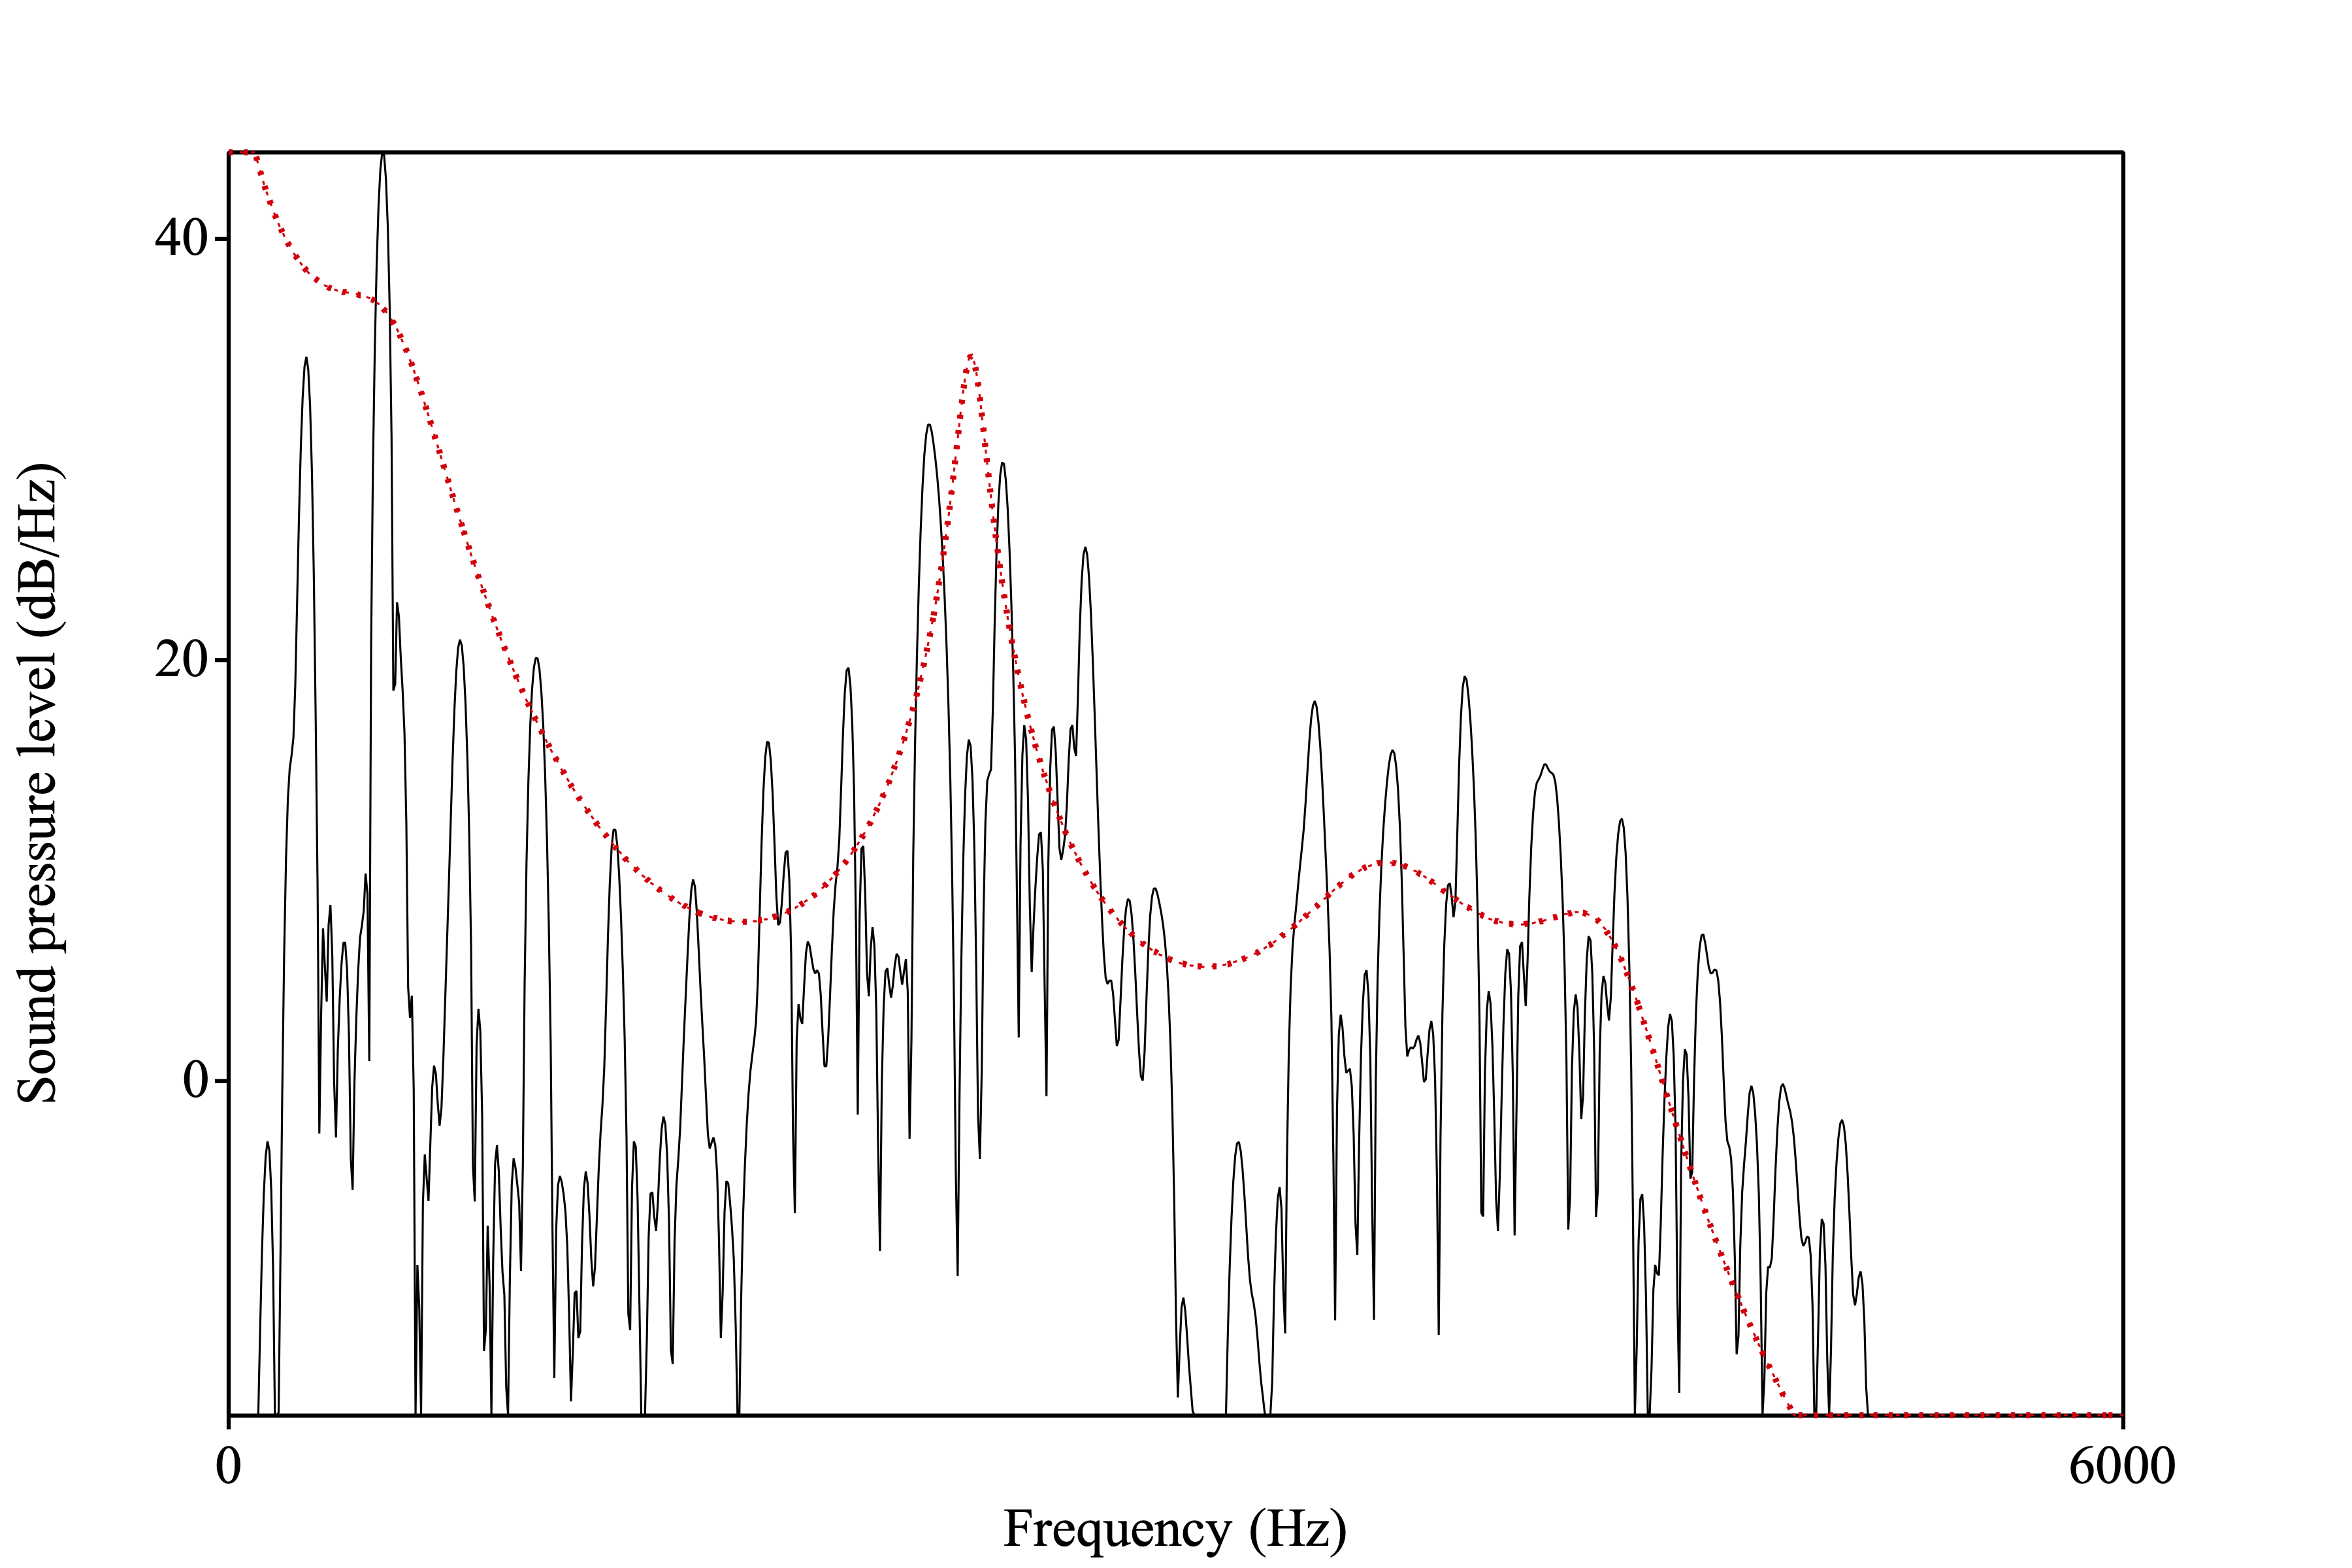
\includegraphics[width=0.9\textwidth]{Images/Harmonics.png}
	\caption{Spectral slice with LPC smoothed line overlaid for the vowel [e]. The harmonics in the spectral slice are represented by each of the dark peaks. The leftmost black solid line peak is the first harmonic (H1), and each subsequent peak represents the next highest harmonic (H2 through H\textit{n}). The red dotted line represents an LPC smoothed line which identifies the formants by the peaks in the line. Each harmonic closest to the formant peak is identified as A1 through A\textit{n}.}
	\label{fig:Harmonics}
\end{figure}

Another spectral-tilt measurement that is sometimes used to differentiate the different phonation types is H1-A3, which is the difference in amplitude between the first harmonic and the amplitude of the harmonic closest to the third formant. One study that made use of this measure is \cite{espositoVariationContrastivePhonation2010}. This study found that in Santa Ana Del Valle Zapotec, a Central Valley Zapotec, phonation contrasts were best captured by different measurements depending on the sex of the speakers. H1-H2 was found to be effective only for female speakers, whereas male speakers were best characterized by H1-A3 for the different phonations that exist in that variety. This pilot study will focus on these two spectral-tilt measurements.

In addition to spectral-tilt measurements, noise measurements frequently accompany phonation investigations (e.g., \cite{garellekPhoneticsWhiteHmong2021}). One of the most commonly used of these noise measurements is Cepstral Peak Prominence (CPP; \cite{hillenbrandAcousticCorrelatesBreathy1994,hillenbrandAcousticCorrelatesBreathy1996}). CPP is similar to the harmonics-to-noise ratio measure of \citet{dekromCepstrumBasedTechniqueDetermining1993} but differs in how the ‘prominence’ of the cepstral peak is calculated. Prominence is taken as the difference in amplitude of the cepstral peak, and a regression line is used to normalize window size and overall energy. In interpreting the measurement, a more prominent cepstral peak indicates stronger harmonics above the spectrum floor (i.e., greater periodicity in the speech signal). CPP was originally used as a diagnostic for breathy or modal voice \citep{blankenshipTimingNonmodalPhonation2002,espositoVariationContrastivePhonation2010} In fact, \citeauthor{espositoEffectsLinguisticExperience2010} showed that CPP was the best of the eight measures she considered for distinguishing modal from breathy phonation types. Further research has shown that CPP is also a good measurement for any type of non-modal phonation (e.g., \cite{andruskiPhonationTypesProduction2000,andruskiToneClarityMixed2006,blankenshipTimingNonmodalPhonation2002,waylandAcousticCorrelatesBreathy2003,avelinoAcousticElectroglottographicAnalyses2010}). This will be the third measurement considered for this pilot study. 

%------------------------------------
\section{Santiago Laxopa Zapotec} \label{sec:SLZ}
%------------------------------------

Santiago Laxopa Zapotec (SLZ; \textit{Dilla'xhunh Laxup}) is a Northern Zapotec language spoken by approximately 1000 people in the municipality of Santiago Laxopa, Ixtlán District in the Sierra Norte of Oaxaca, Mexico \citep{adlerAcousticsPhonationTypes2016,adlerDerivationVerbInitiality2018,foleyForbiddenCliticClusters2018,foleyExtendingPersonCaseConstraint2020}. It is closely related to San Bartolomé Zoogocho Zapotec \citep{longDiccionarioZapotecoSan2005,sonnenscheinDescriptiveGrammarSan2005} and is mutually intelligible with this variety according to native speakers.  As is common among Zapotecan languages, SLZ distinguishes between lenis and fortis consonants \citep[e.g.,][]{nellisFortisLenisCajonos1980,jaegerFortisLenisQuestion1983,uchiharaFortisLenisGlides2016} and has a fairly standard five-vowel inventory, see Table~\ref{tab:SLZcons} and Table~\ref{tab:SLZvowels}.\footnote{The consonant and vowel inventories was previously established by the Zapotec Language Project at UCSC (\url{https://zapotec.ucsc.edu/}) }

\begin{table}[!h]
	\centering
	\caption{Consonant inventory for Santiago Laxopa Zapotec}
	\label{tab:SLZcons}
	\fittable{
	\begin{tabular}{llcccccccc}
	\lsptoprule
		  &  & bilabial & alveolar  & post- & retroflex & palatal &velar &labio-  &  uvular \\
		 &&&&alveolar&  &&&velar& \\
	\midrule
	stop 	& lenis   & b  & d  & & & & g & gʷ & \\
				& fortis  & p  & t  & & & & k & kʷ & \\
	fricative   & lenis   &    & z  & ʒ & ʐ &  & &  & ʁ \\
		        & fortis  &    & s  & ʃ & ʂ & ç & & & \\
	affricate 	& lenis   &    & d͡z & & & & & & \\
				& fortis  &    & t͡s & & t͡ʃ & & & & \\
        nasal	& lenis   &	   & n  & & & & & & \\
				& fortis  &	mː & nː & & & & & & \\
	lateral  	& lenis   &    & l & & & & & & \\
				& fortis  &    & lː & & & & & & \\
	trill		& 		  &    & r & & &  & &  & \\ 			
	approximate & 		  &    & & & & & & w & \\ 
	\lspbottomrule
	\end{tabular}
	}
\end{table}

	\begin{table}[!h]
		\centering
		\caption{Vowels inventory in Santiago Laxopa Zapotec.}
		\label{tab:SLZvowels}
		 \begin{tabular}{lccc}
		  \lsptoprule
					&  front& central  & back \\
		  \midrule
			high   	&  i  &     &   u \\
			mid    	&  e  &   	& 	o \\
			low   	&     &  a 	&	  \\
		  \lspbottomrule
		 \end{tabular}
		\end{table}
		
In addition to the contrasts in both consonants and vowels, SLZ additionally has both a phonation and tonal contrast. I will first talk about the tonal contrasts in Section~\ref{sec:Tone} followed by the tonal phonation in Section~\ref{sec:Phonation}.

%------------------------------------
\subsection{Tone in SLZ} \label{sec:Tone}
%------------------------------------

As is common among Oto-Manguean languages, SLZ is a tonal language \citep{suarezMesoamericanIndianLanguages1983,campbellMesoAmericaLinguisticArea1986,silvermanLaryngealComplexityOtomanguean1997,campbellOtomangueanHistoricalLinguistics2017a,campbellOtomangueanHistoricalLinguistics2017}. 
This paper represents the first time that a detailed description of the tone system has been presented in writing. Previous studies by the Zapotec Language Project at UCSC on the tonal system were heavily based on the closely related San Bartolomé Zoogocho Zapotec \citep{longDiccionarioZapotecoSan2005,sonnenscheinDescriptiveGrammarSan2005}. 
San Bartolomé Zoogocho Zapotec has been previously described as having as few as 6 tones \citep{sonnenscheinDescriptiveGrammarSan2005} and as many as eleven tones \citep{longDiccionarioZapotecoSan2005}. 
In order to determine the exact number of tones in SLZ, a combination of \posscitet{pikeToneLanguagesTechnique1948} method for discovering tonal contrasts and \posscitet{sniderEstablishingUnderlyingTonal2014} method of compiling a tonal database of words and their tonal patterns in different phrases and contexts. Based on this research, SLZ has five surface tones that appear on a syllable; see Table~\ref{tab:tones}. 

\begin{table}[!h]
	\centering
	\caption{Examples of the five tonal patterns observed in the Santiago Laxopa Zapotec words.}
	\label{tab:tones}
	 \begin{tabular}{lllll}
	  \lsptoprule
					  % &	 Diacritic  & Example & Transcription \\
	  High   	&  a\supr{H}  &  \textit{xha}   &  [ ʐa\supr{H} ] & `clothing.\textsc{poss}'\\
		Mid    	&  a\supr{M}  &  \textit{lhill} 	& [ liʒ\supr{M} ] & `house.\textsc{poss}' \\
		Low   	&  a\supr{L}  &  \textit{yu'} 	&	 [ çuˀ\supr{L} ] & `earth'\\
		Rising	&  a\supr{MH}  &  \textit{yu'u} 	&	[ çuˀu\supr{MH} ] & `quicklime (Sp. cal)' \\
		Falling &  a\supr{HL}  &  \textit{yu'u}  &	[çuˀu\supr{HL}] &	`house' \\
	  \lspbottomrule
	 \end{tabular}
\end{table}

Several sets of (near-)minimal pairs and triplets can present the syllable's full range of tonal contrasts. The first minimal pair consists of the words \textit{yu'u} [çuˀu\supr{MH}] `quicklime' and \textit{yu'u} [çuˀu\supr{HL}] `house'. In this pair of words, the only difference is whether you have a rising or falling tone on the word, with `quicklime' having a rising tone and `house' a falling tone. Additionally, we can establish three unique tones by including the near minimal word \textit{yu'} [çuˀ\supr{L}] `earth', which bears a low tone. 

The mid and high rarely appear on monosyllabic nominals but frequently appear as part of bisyllabic words. The few examples of monosyllabic words that contain these tones often have these tones supplanted by other tones. This is because they are special possessive forms of nouns that must bear clitic pronouns or be combined with a possessive phrase. These clitic pronouns all bear their own tones, which supplant the tones of their host. In the case of the mid-toned word \textit{lhill} [ɾiʒ\supr{M}] `house.\Poss{}{}', if the first person singular clitic pronoun \textit{-a'} [\supr{H}-aˀ] appears attached to the word (\textit{lhilla'} [ɾiʒ-aˀ\supr{HL}]) only a high tone is present on the root, most of the other clitic pronouns have low tones that also override the tone of possessed nouns. This overriding is because the first person singular has a floating high tone that attaches to the root; this is also true with verbs. If \textit{lhill} is possessed by another noun such as \textit{beku'} `dog' in the phrase \textit{lhill tse beku'nh} [ɾiʒ\supr{M} tse\supr{M} bekuˀ\supr{HL}] `the dog's house' the underlying tone of the word is allowed to surface. This is also true for the few monosyllabic high-toned words such as \textit{xha} [ʐa\supr{H}] `clothing.\Poss{}{}'.

In addition to these facts in the nominal domain, High-tone and mid-tone are very present in other domains. Mid-tone is very common among numerals, and high-tone is frequently part of verbal morphology as the primary cue for the potential aspect.

\begin{figure}[!ht]
	\centering
	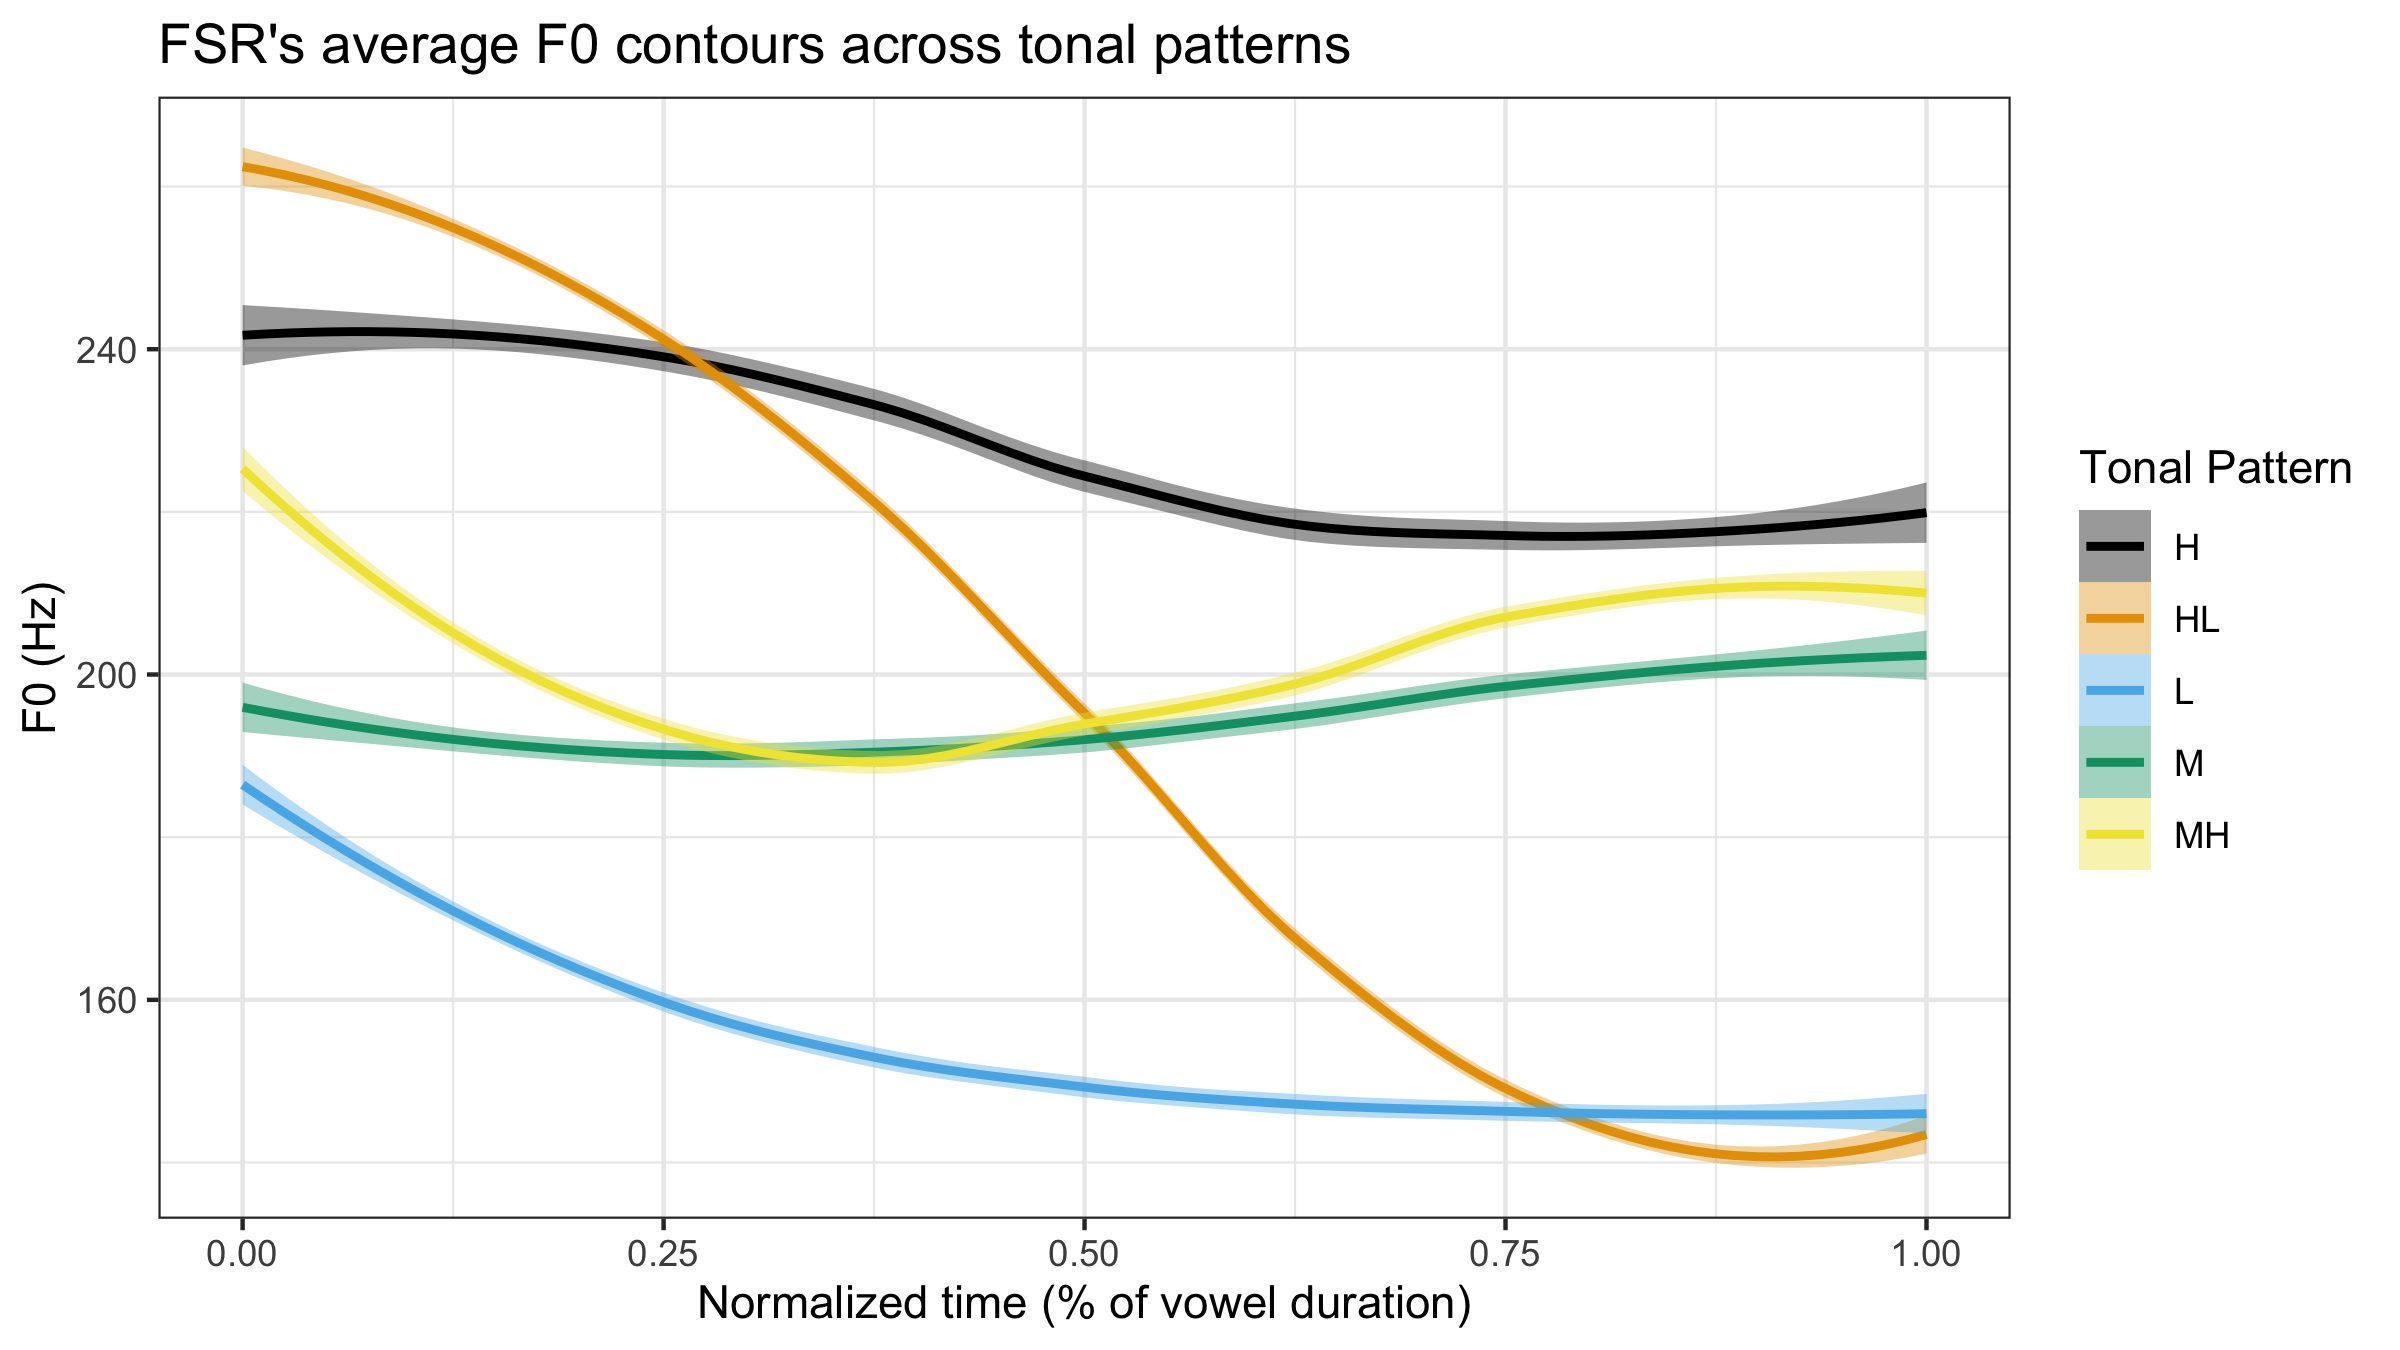
\includegraphics[width=0.9\textwidth]{Images/FSRTonePlot.png}
	\label{fig:FSRTonePlot}
	\caption{Tonal contrasts for FSR averaged and time normalized. Each line in this graph represents the average of approximately 10 syllables for that tonal pattern. }
\end{figure}

\begin{figure}[!ht]
	\centering
	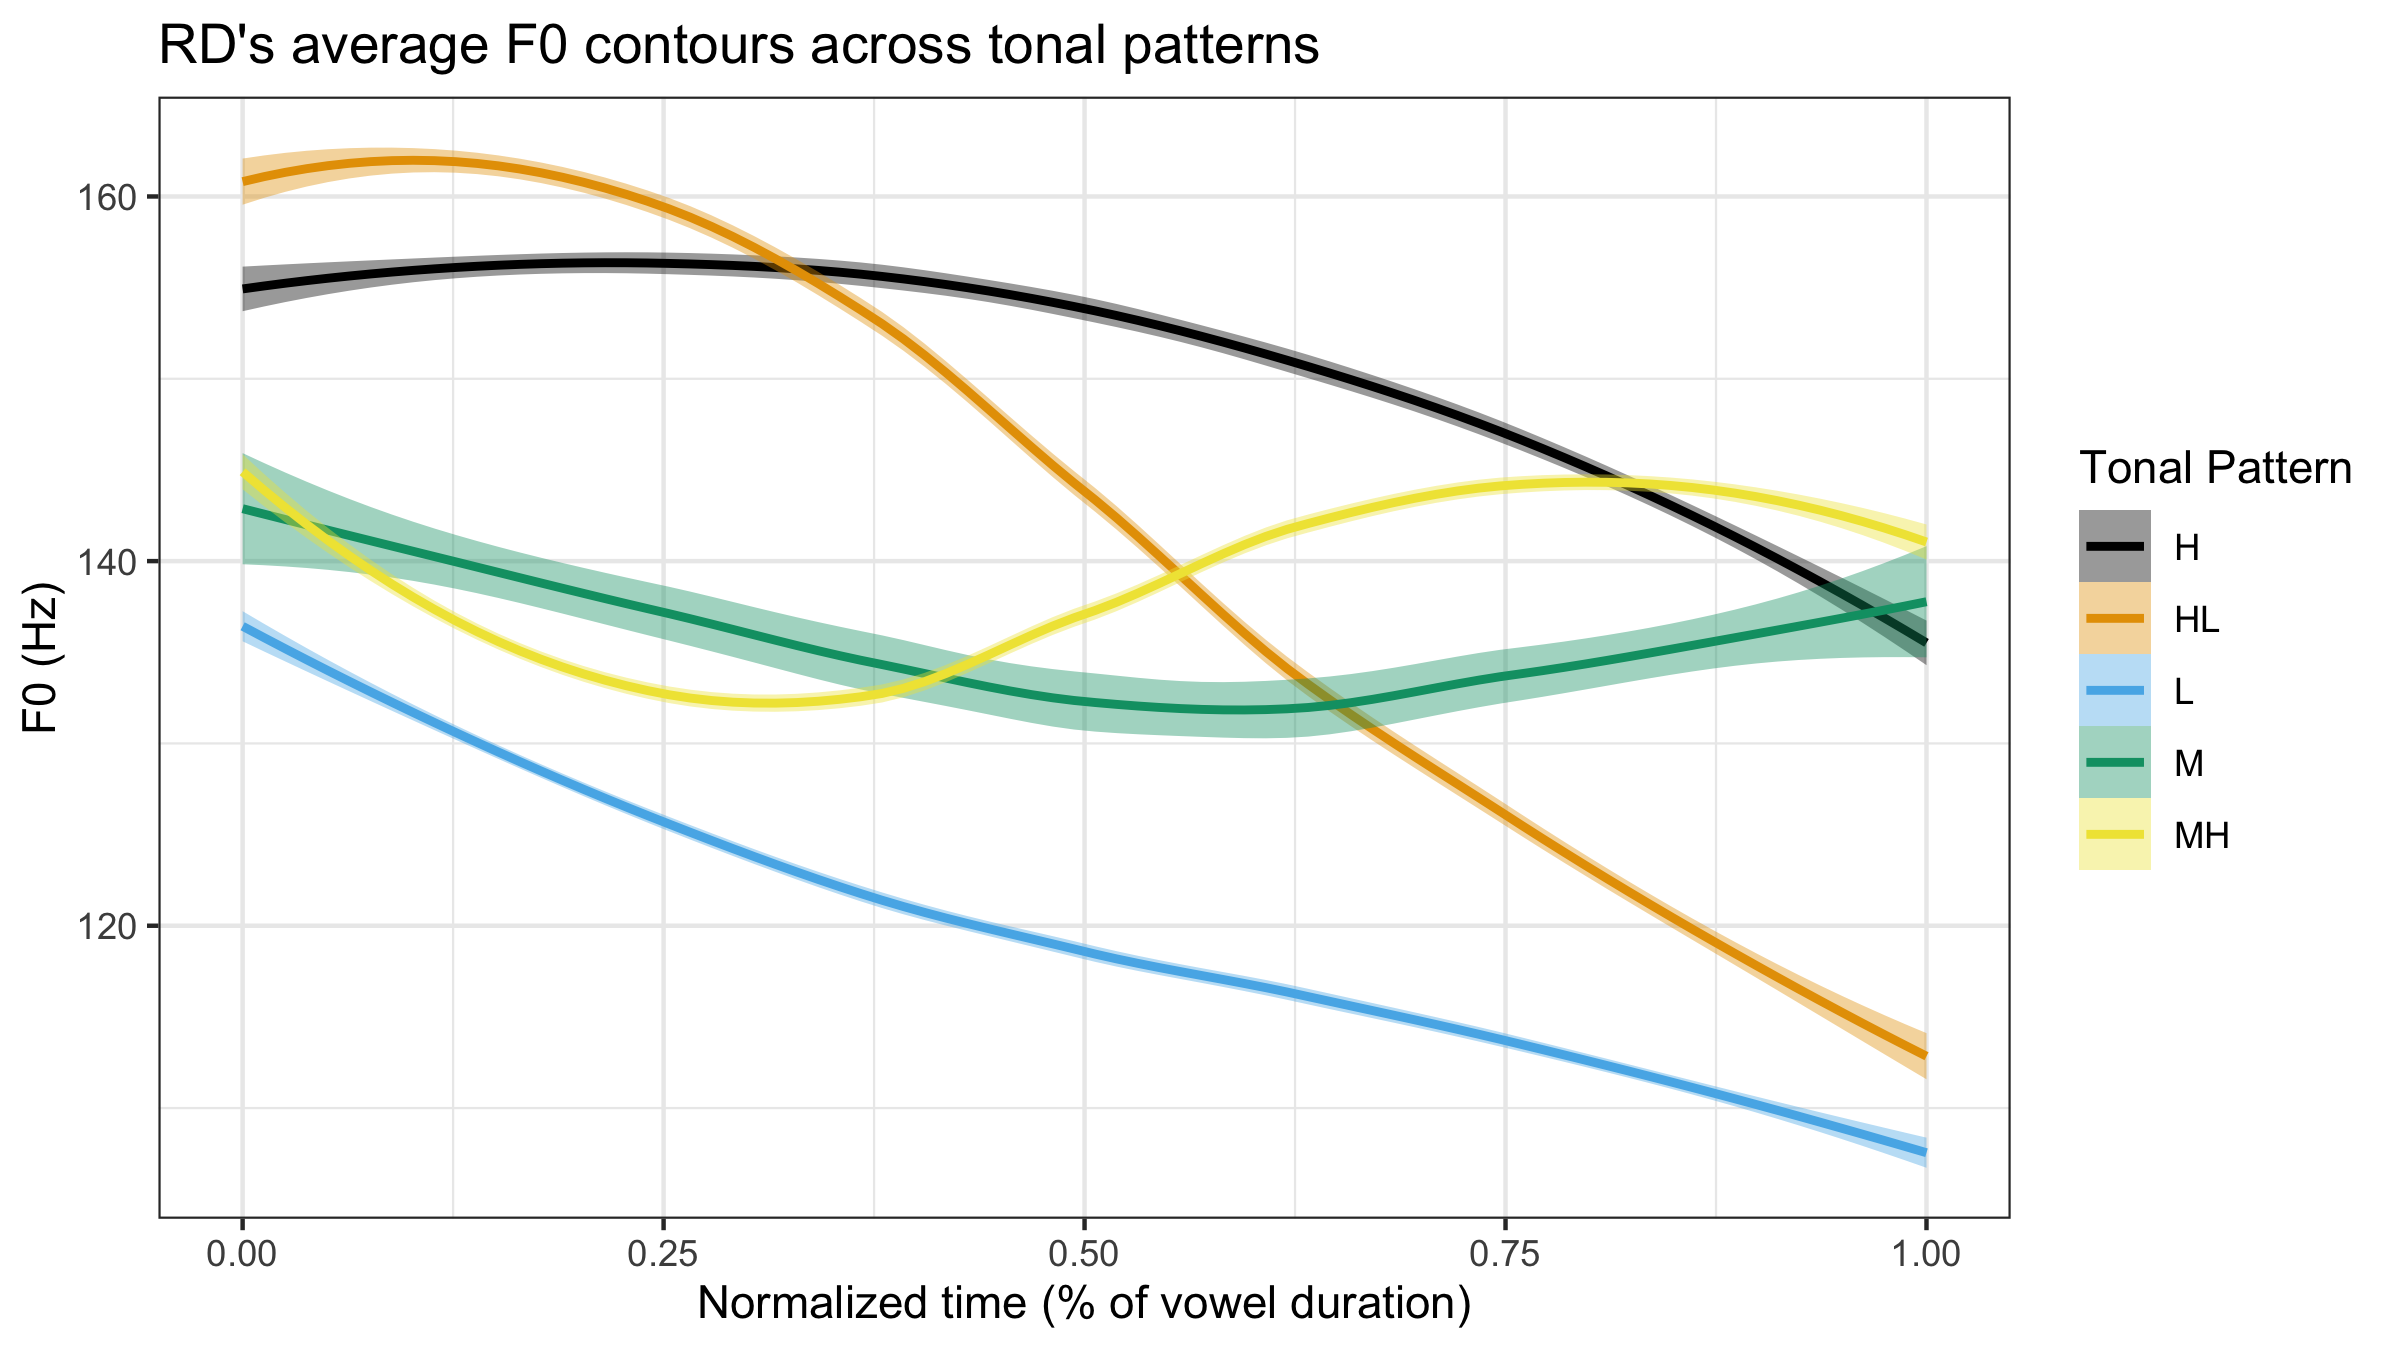
\includegraphics[width=0.9\textwidth]{Images/RDTonePlot.png}
	\label{fig:RDTonePlot}
	\caption{Tonal contrasts for RD averaged and time normalized. Each line in this graph represents the average of approximately 10 syllables for that tonal pattern.}
\end{figure}

Following discussion from \citet{brinkerhoffTonalPatternsTheir2022} these tones appear to be limited in their distribution. It is true that all five patterns can surface on a syllable, but there is a restriction on what tonal patterns are allowed to surface on words that are larger than bimoraic. The patterns observed on bimoraic nominals are HL, MH, and LL.

%------------------------------------
\subsection{Phonation in SLZ} \label{sec:Phonation}
%------------------------------------

Among Zapotecan languages, it is quite common for languages to make use of contrastive phonation \citep[e.g.,][]{avelinobecerraTopicsYalalagZapotec2004,longDiccionarioZapotecoSan2005,avelinoAcousticElectroglottographicAnalyses2010,lopeznicolasEstudiosFonologiaGramatica2016,chavez-peonInteractionMetricalStructure2010}. 
SLZ, in addition to the five vowel qualities, has four contrastive phonation types: modal, breathy, checked, and laryngealized. These contrasts are exemplified in the minimal quadruple in (\ref{ex:YA}). In representing the checked and laryngealized vowels, I follow the same procedure as other authors (e.g., \citet{avelinoAcousticElectroglottographicAnalyses2010, uchiharaToneRegistrogenesisQuiavini2016}) in representing the `glottal stop' element as a superscript glottal stop in the IPA transcription (i.e., [aˀ]). This is primarily done as a way of standardizing the variable pronunciation of the glottal element in Zapotec, ranging from a full glottal stop (i.e., [aʔ]) to a creaky portion of the vowel (i.e., [aa̰]).  

\ea \label{ex:YA} Four-way near minimal phonation contrast
	\ea \textit{yag}  /çag\supr{L}/ `tree; wood; almúd (unit of measurement approximately 4kg)'
	\ex \textit{yah}  /ça̤\supr{L}/ `metal; rifle; bell'
	\ex \textit{yu'}  /çuˀ\supr{L}/  `earth'
	\ex \textit{ya'a}  /çaˀa\supr{L}/  `market'
	\z 
\z 

Breathy phonation on vowels is characterized by a raspy quality throughout the whole vowel or a portion toward the end of the vowel; see Figure~\ref{fig:BreathyVowel}. 

\begin{figure}[!h]
	\centering
	% [INSERT YAH SPECTROGRAM AND WAVEFORM]
	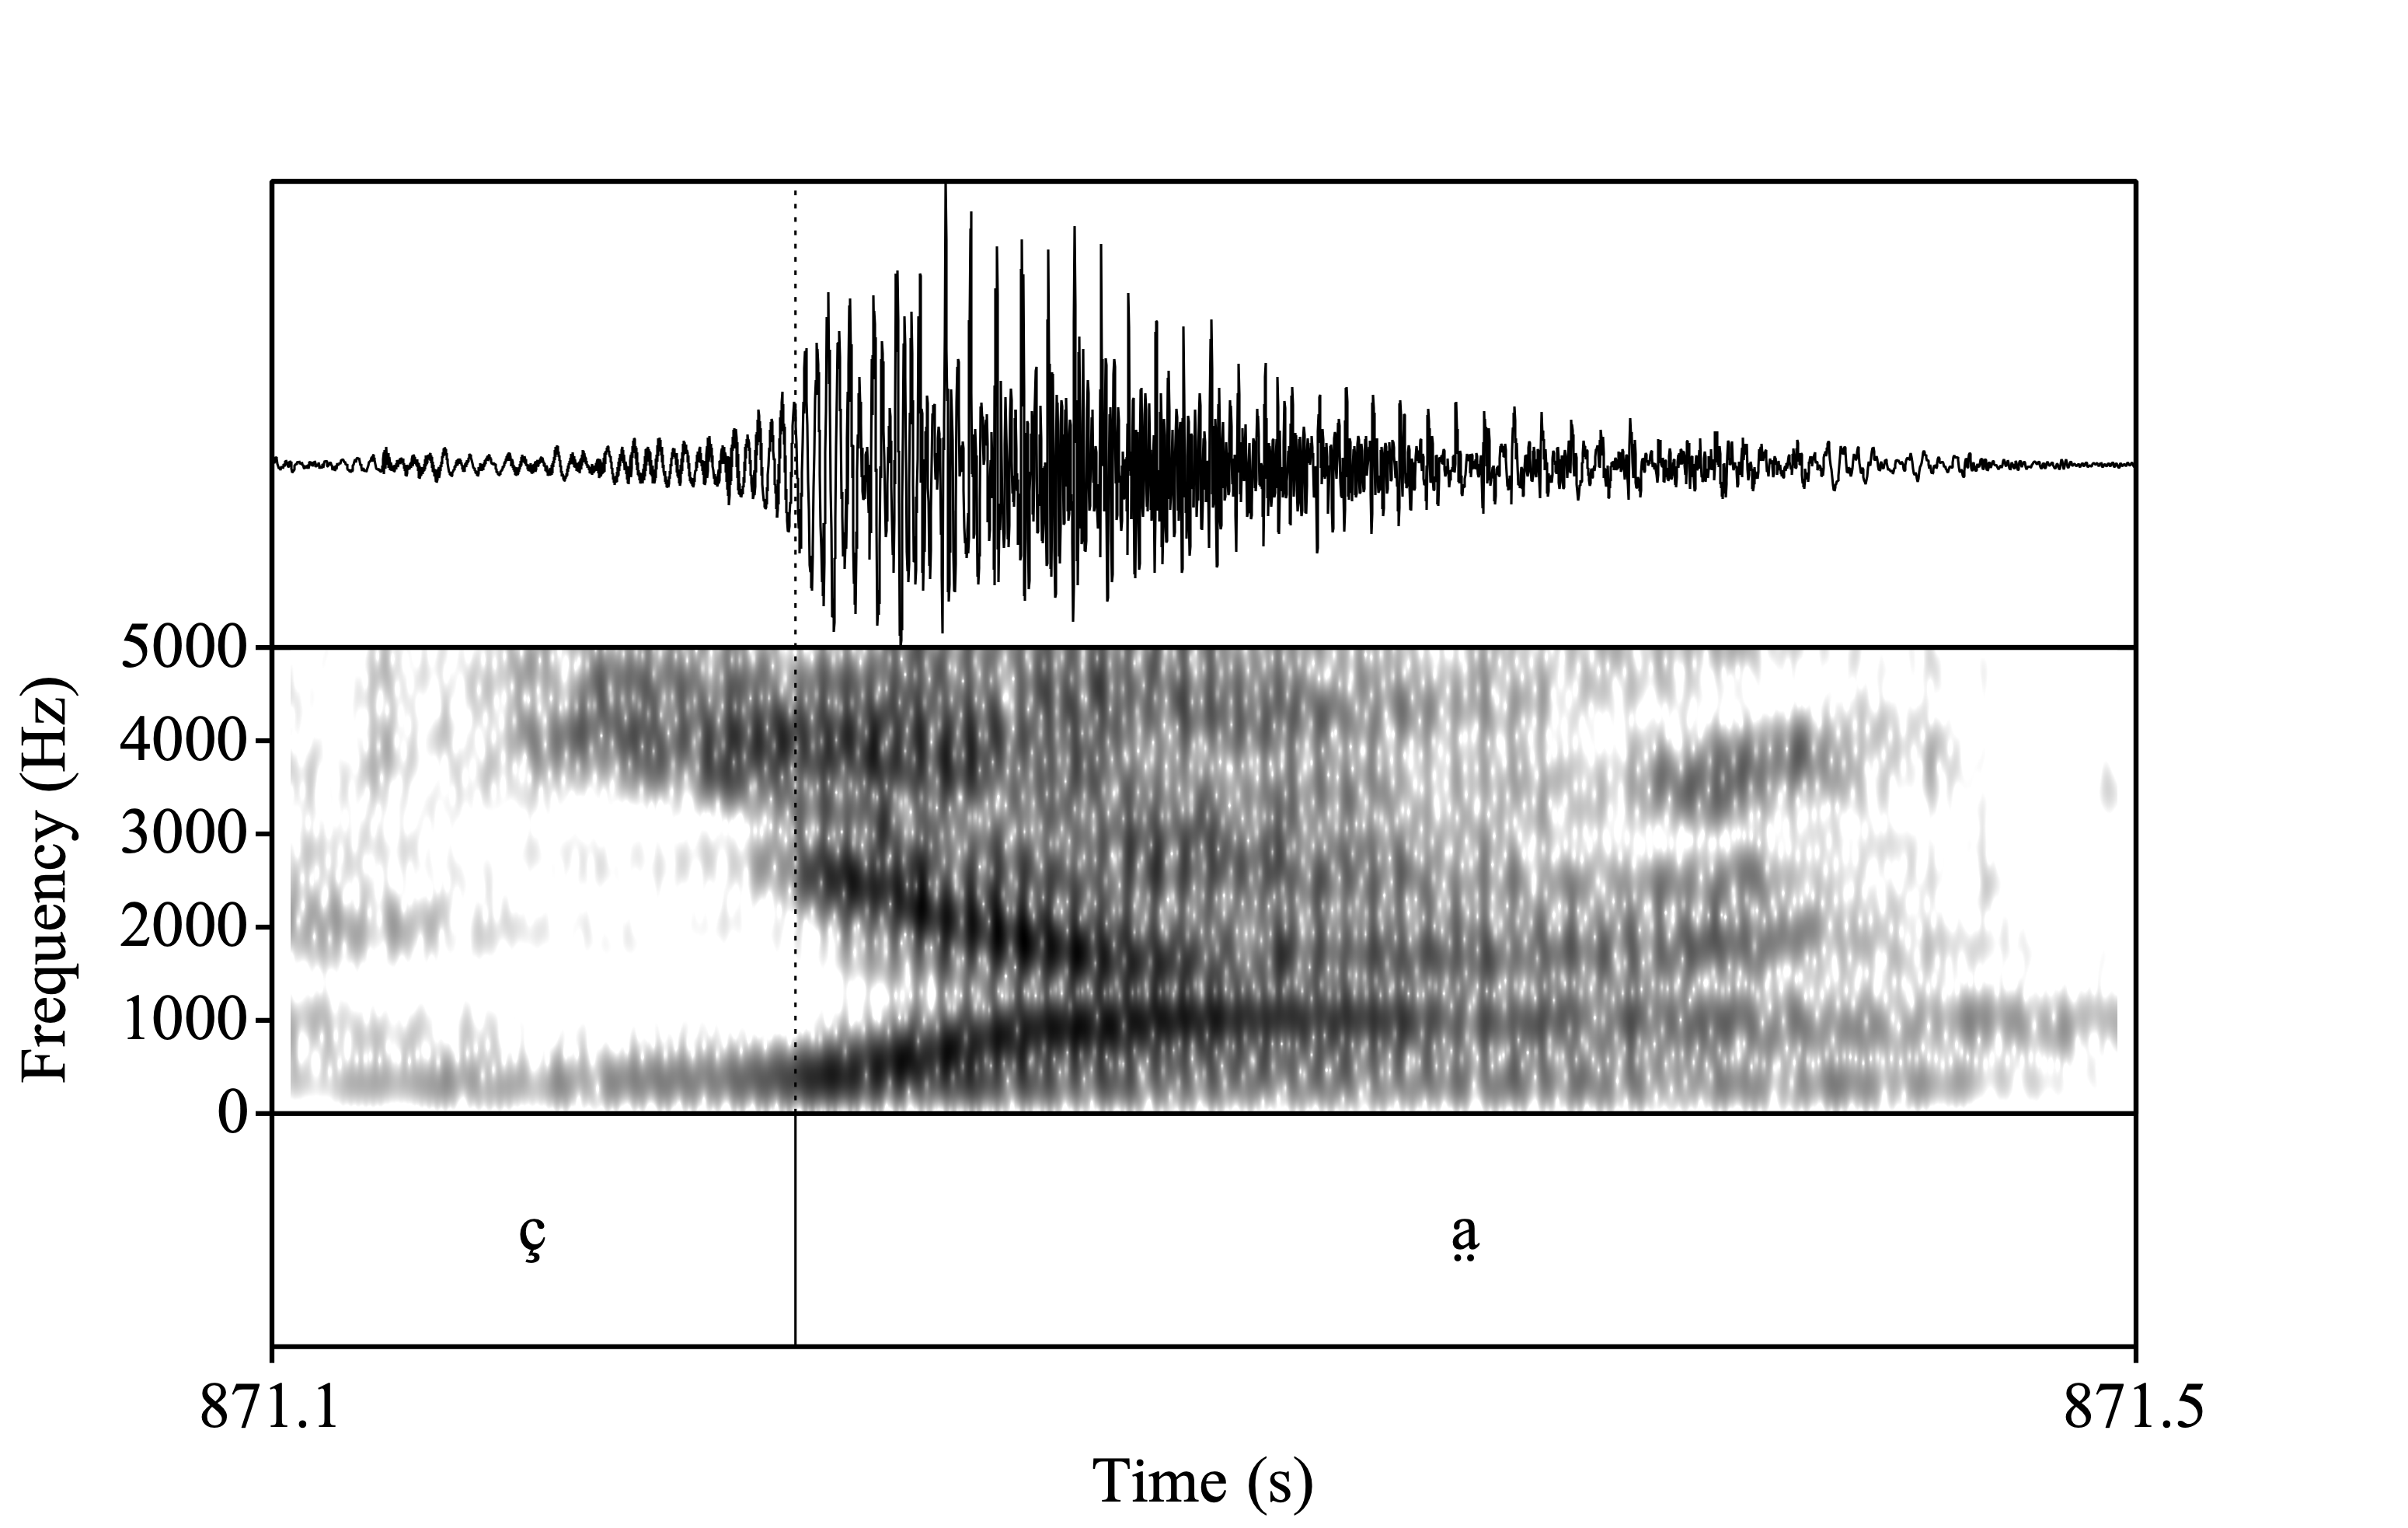
\includegraphics[width=0.9\textwidth]{Images/yah.png}
	\caption{Breathy vowel in the word \textit{yah} `metal; rifle'}
	\label{fig:BreathyVowel}
\end{figure}

On the other hand, checked vowels are characterized by an abrupt glottal closure which cuts the vowel short. This phonation is sometimes only realized as a very short period of creakiness at the end of the vowel; see Figure~\ref{fig:CheckedVowel}.  

\begin{figure}[!h]
	\centering
	% [INSERT YA SPECTROGRAM AND WAVEFORM]
	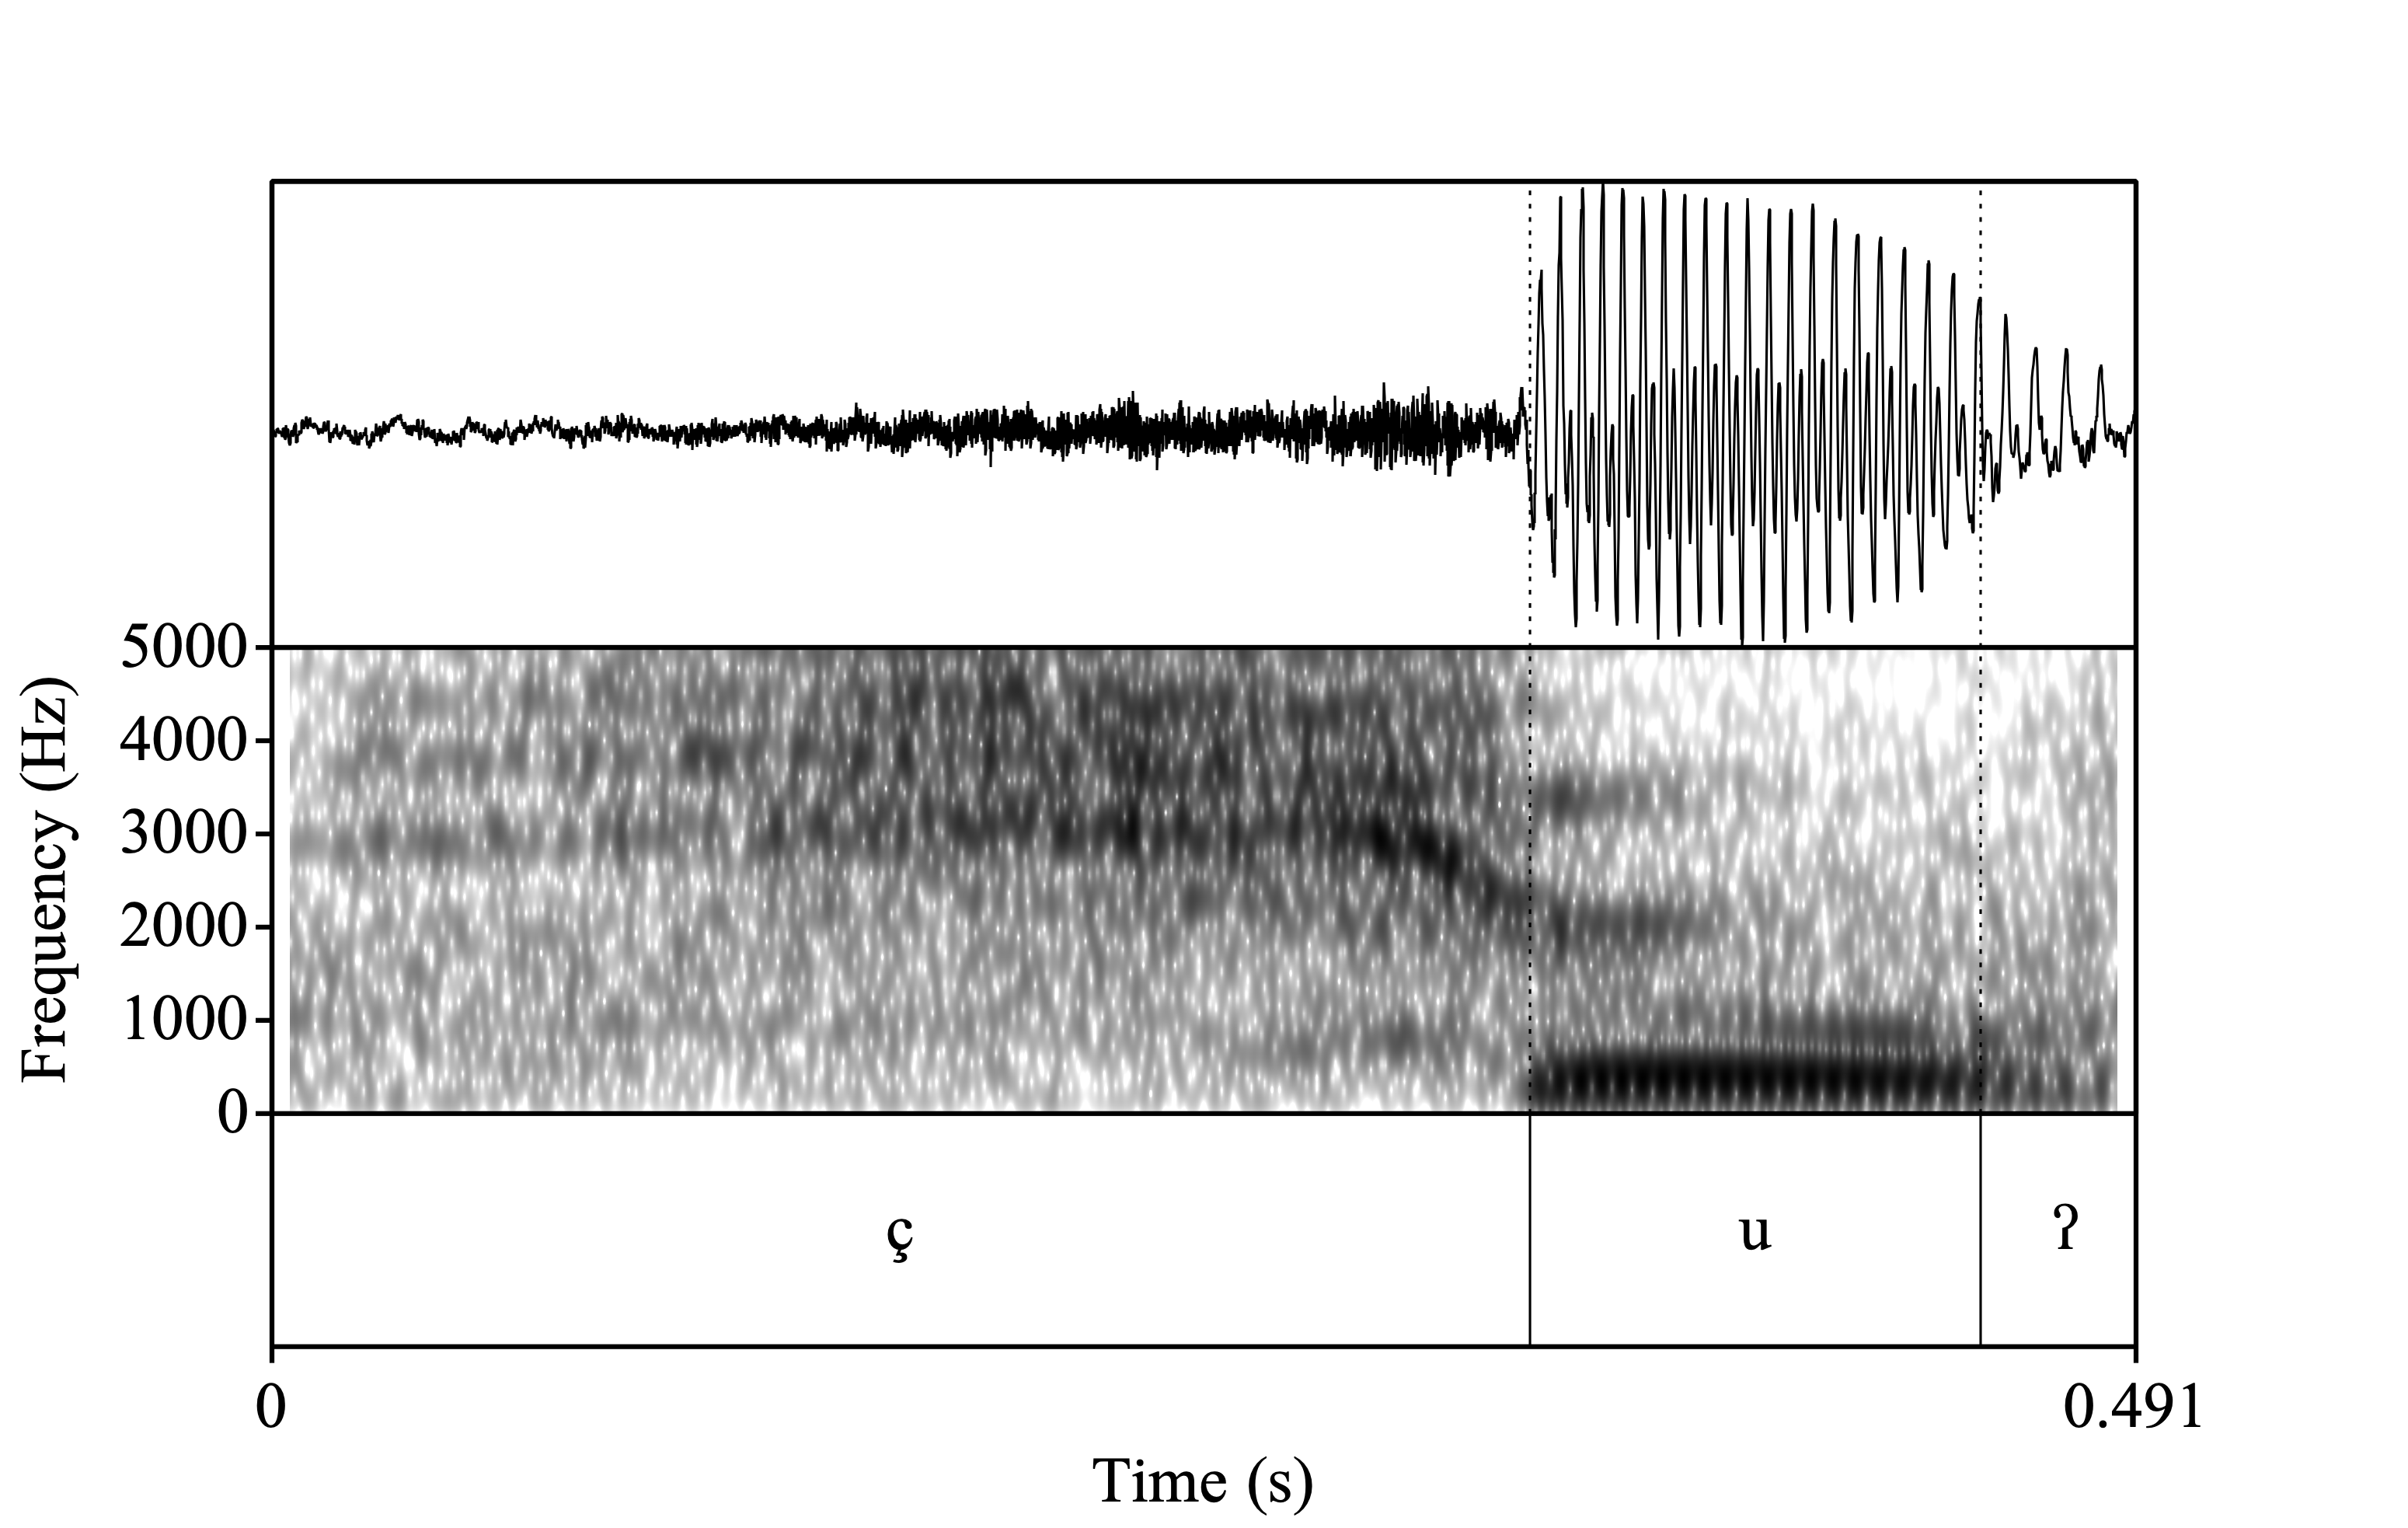
\includegraphics[width=0.9\textwidth]{Images/RD_yu'.png}
	\caption{Checked vowel in the word \textit{yu'} `earth'}
	\label{fig:CheckedVowel}
\end{figure}

Laryngealized vowels are quite common in Zapotecan languages and have received a wide number of different names. Previous descriptions have used terms such as broken, rearticulated, interrupted, and creaky \citep{longDiccionarioZapotecoSan2005,avelinobecerraTopicsYalalagZapotec2004,avelinoAcousticElectroglottographicAnalyses2010,sonnenscheinDescriptiveGrammarSan2005,adlerAcousticsPhonationTypes2016}. To avoid confusion; I will use the term laryngealized following \citet{avelinoAcousticElectroglottographicAnalyses2010}. In addition to many different names, these vowels also exhibit a wide range of allophones. 

\citet{avelinoAcousticElectroglottographicAnalyses2010} found in the closely related Yalálag Zapotec that among his consultants, there were at least four different pronunciations as seen in Table~\ref{tab:laryngeal}. 
\begin{table}[!h]
	\centering
	\caption{Layngealized Vowels in Yalálag Zapotec}
	\label{tab:laryngeal}
	 \begin{tabular}{ll}
	\lsptoprule
	/VˀV/	&  [VʔV]  \\
			&  [VV̰V]   \\
			&  [VV̰ːV̆]  \\
			&  [VV̰V̰]	\\
	\lspbottomrule
	\end{tabular}
\end{table}
In SLZ, each consulted language expert would produce this vowel differently. One consultant would re-articulate, where there is a full glottal stop in the middle of the vowel, or they would produce creaky voice. This alternation seemed to be in free variation, but there was a greater tendency to creak in low-toned words, such as \textit{xa'ag} [ʂa̰ːg] `topil'\footnote{A \textit{topil} is a type of government office in traditional Oaxacan communities somewhat akin to a sheriff.}, see Figure~\ref{fig:FSRLaryngeal} for a comparison between this consultant's pronunciation of the laryngealized vowels.

\begin{figure}[!h]
	\centering
	\begin{subfigure}{.5\textwidth}
		\centering
		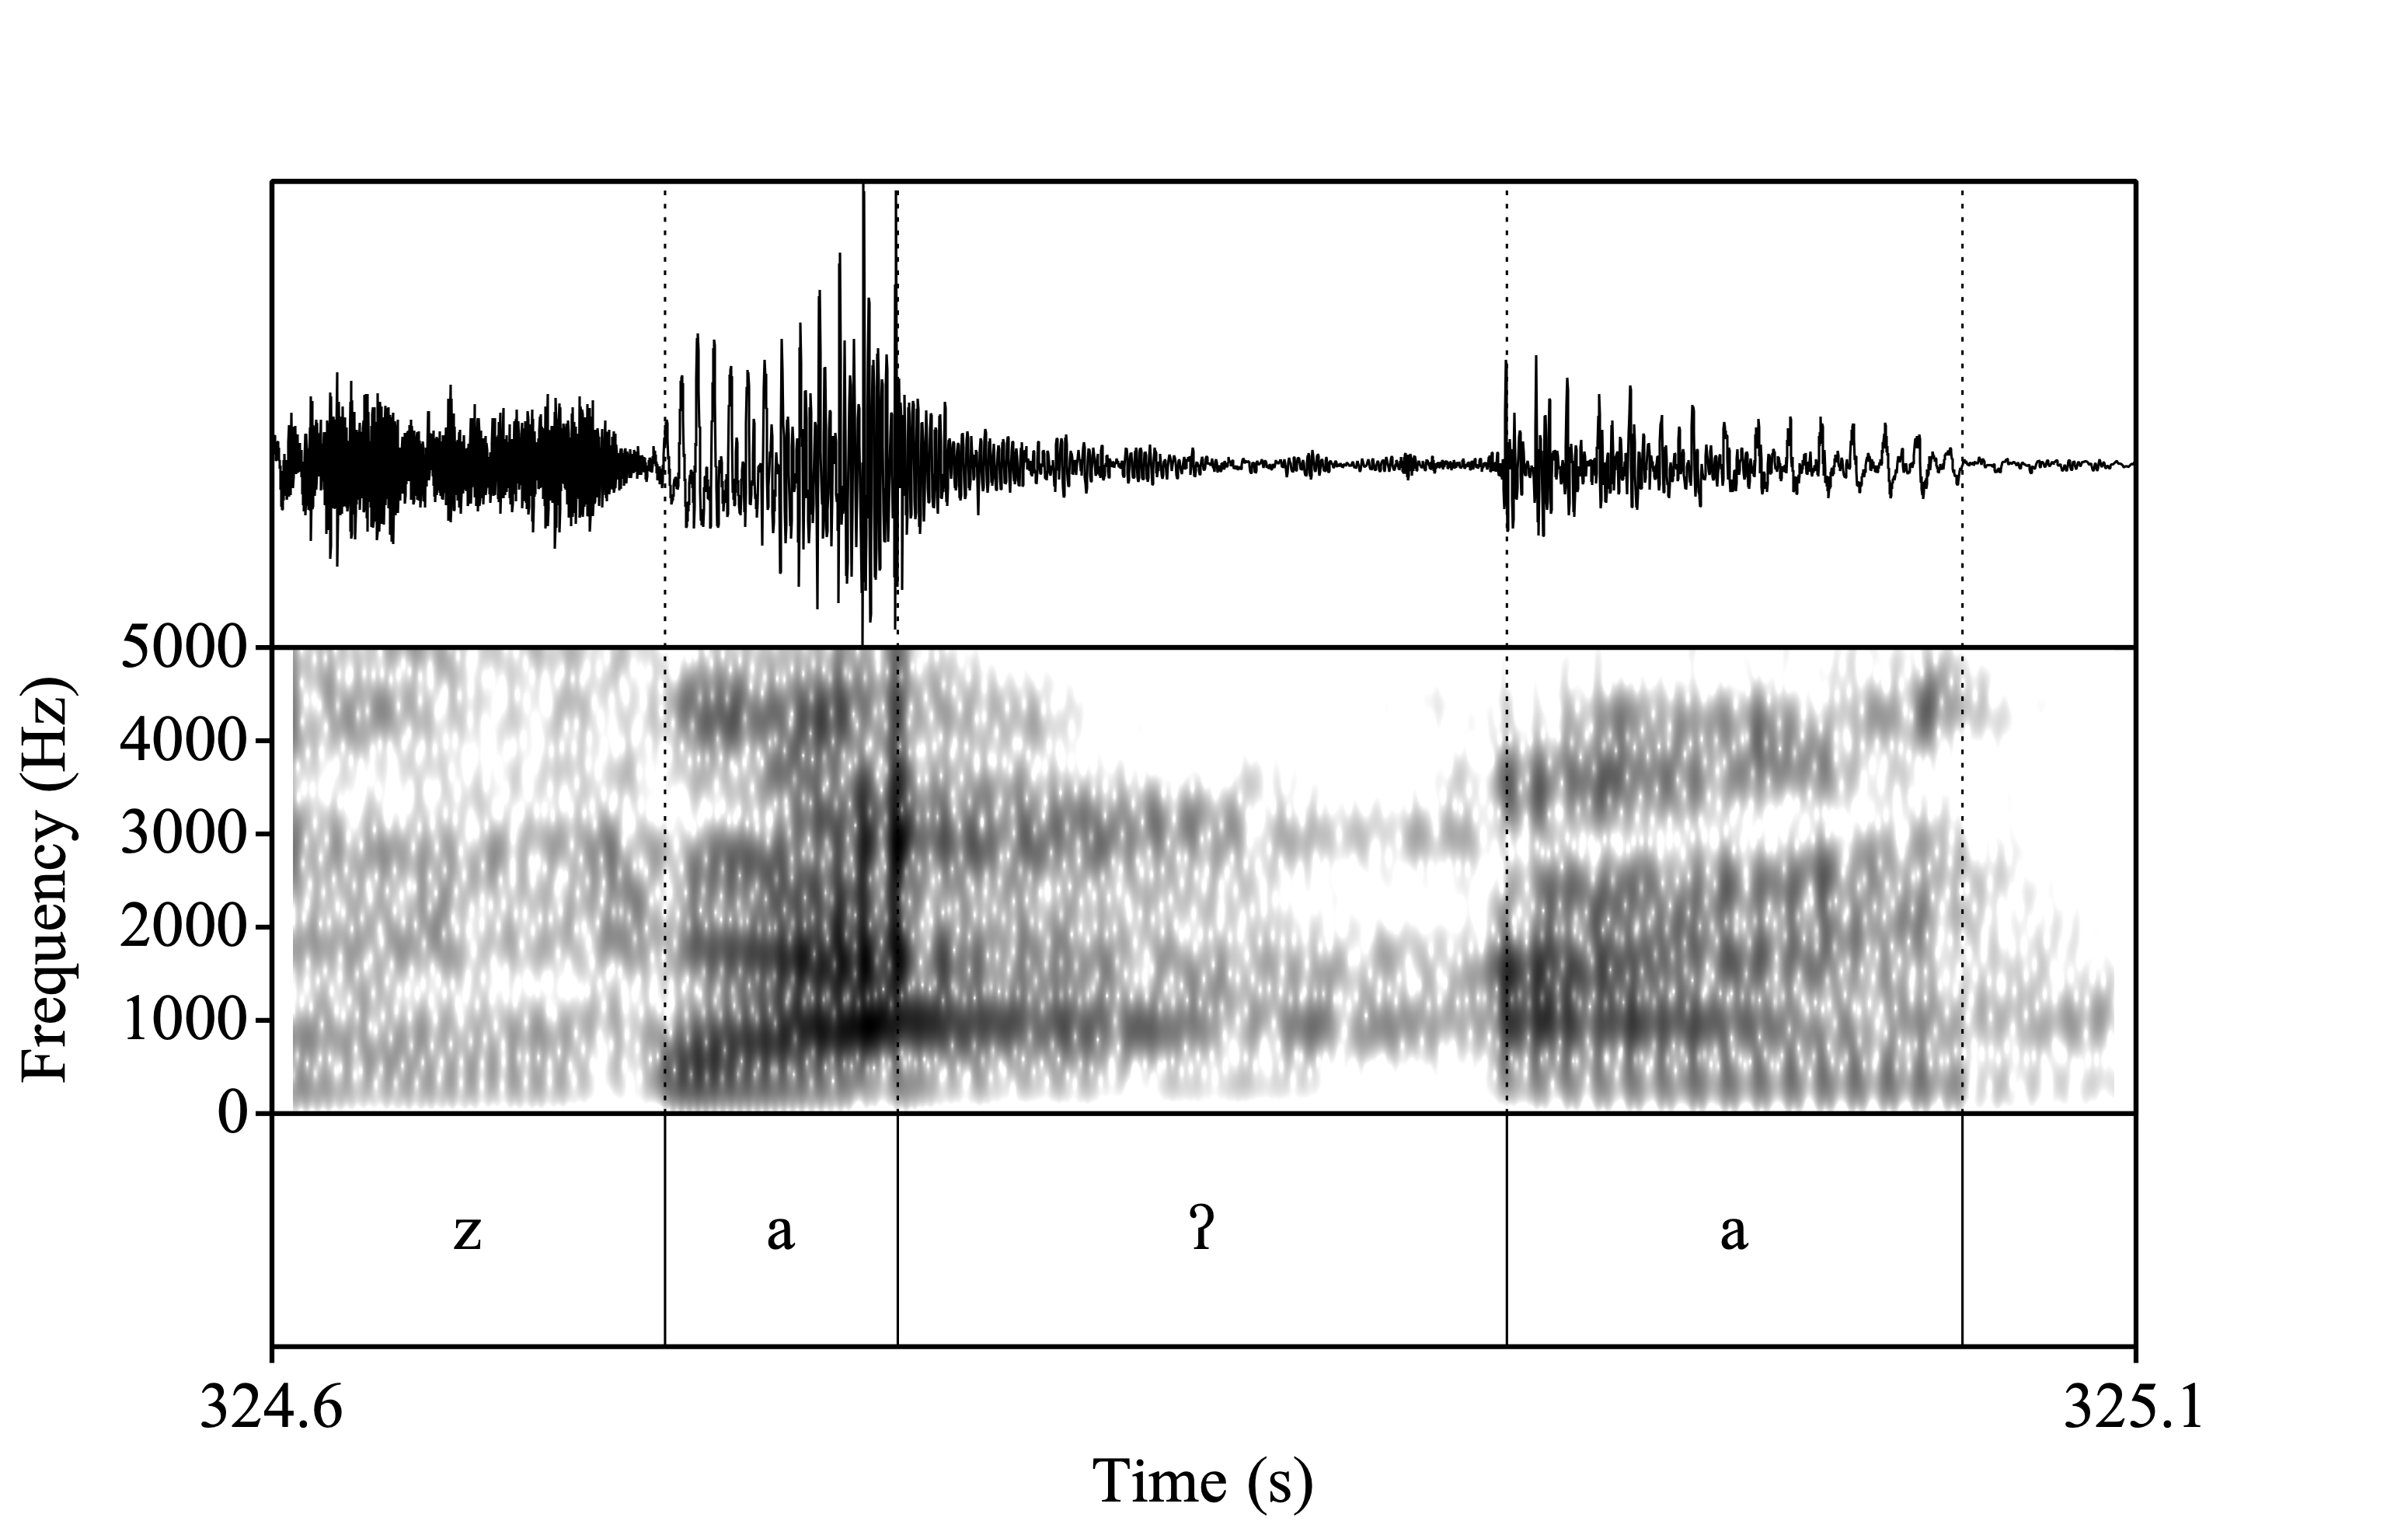
\includegraphics[width=\linewidth]{Images/za'a.png}
		\caption{\textit{za'a} `corncob'}
		\label{fig:za'a}
	\end{subfigure}%
	\begin{subfigure}{.5\textwidth}
		\centering
		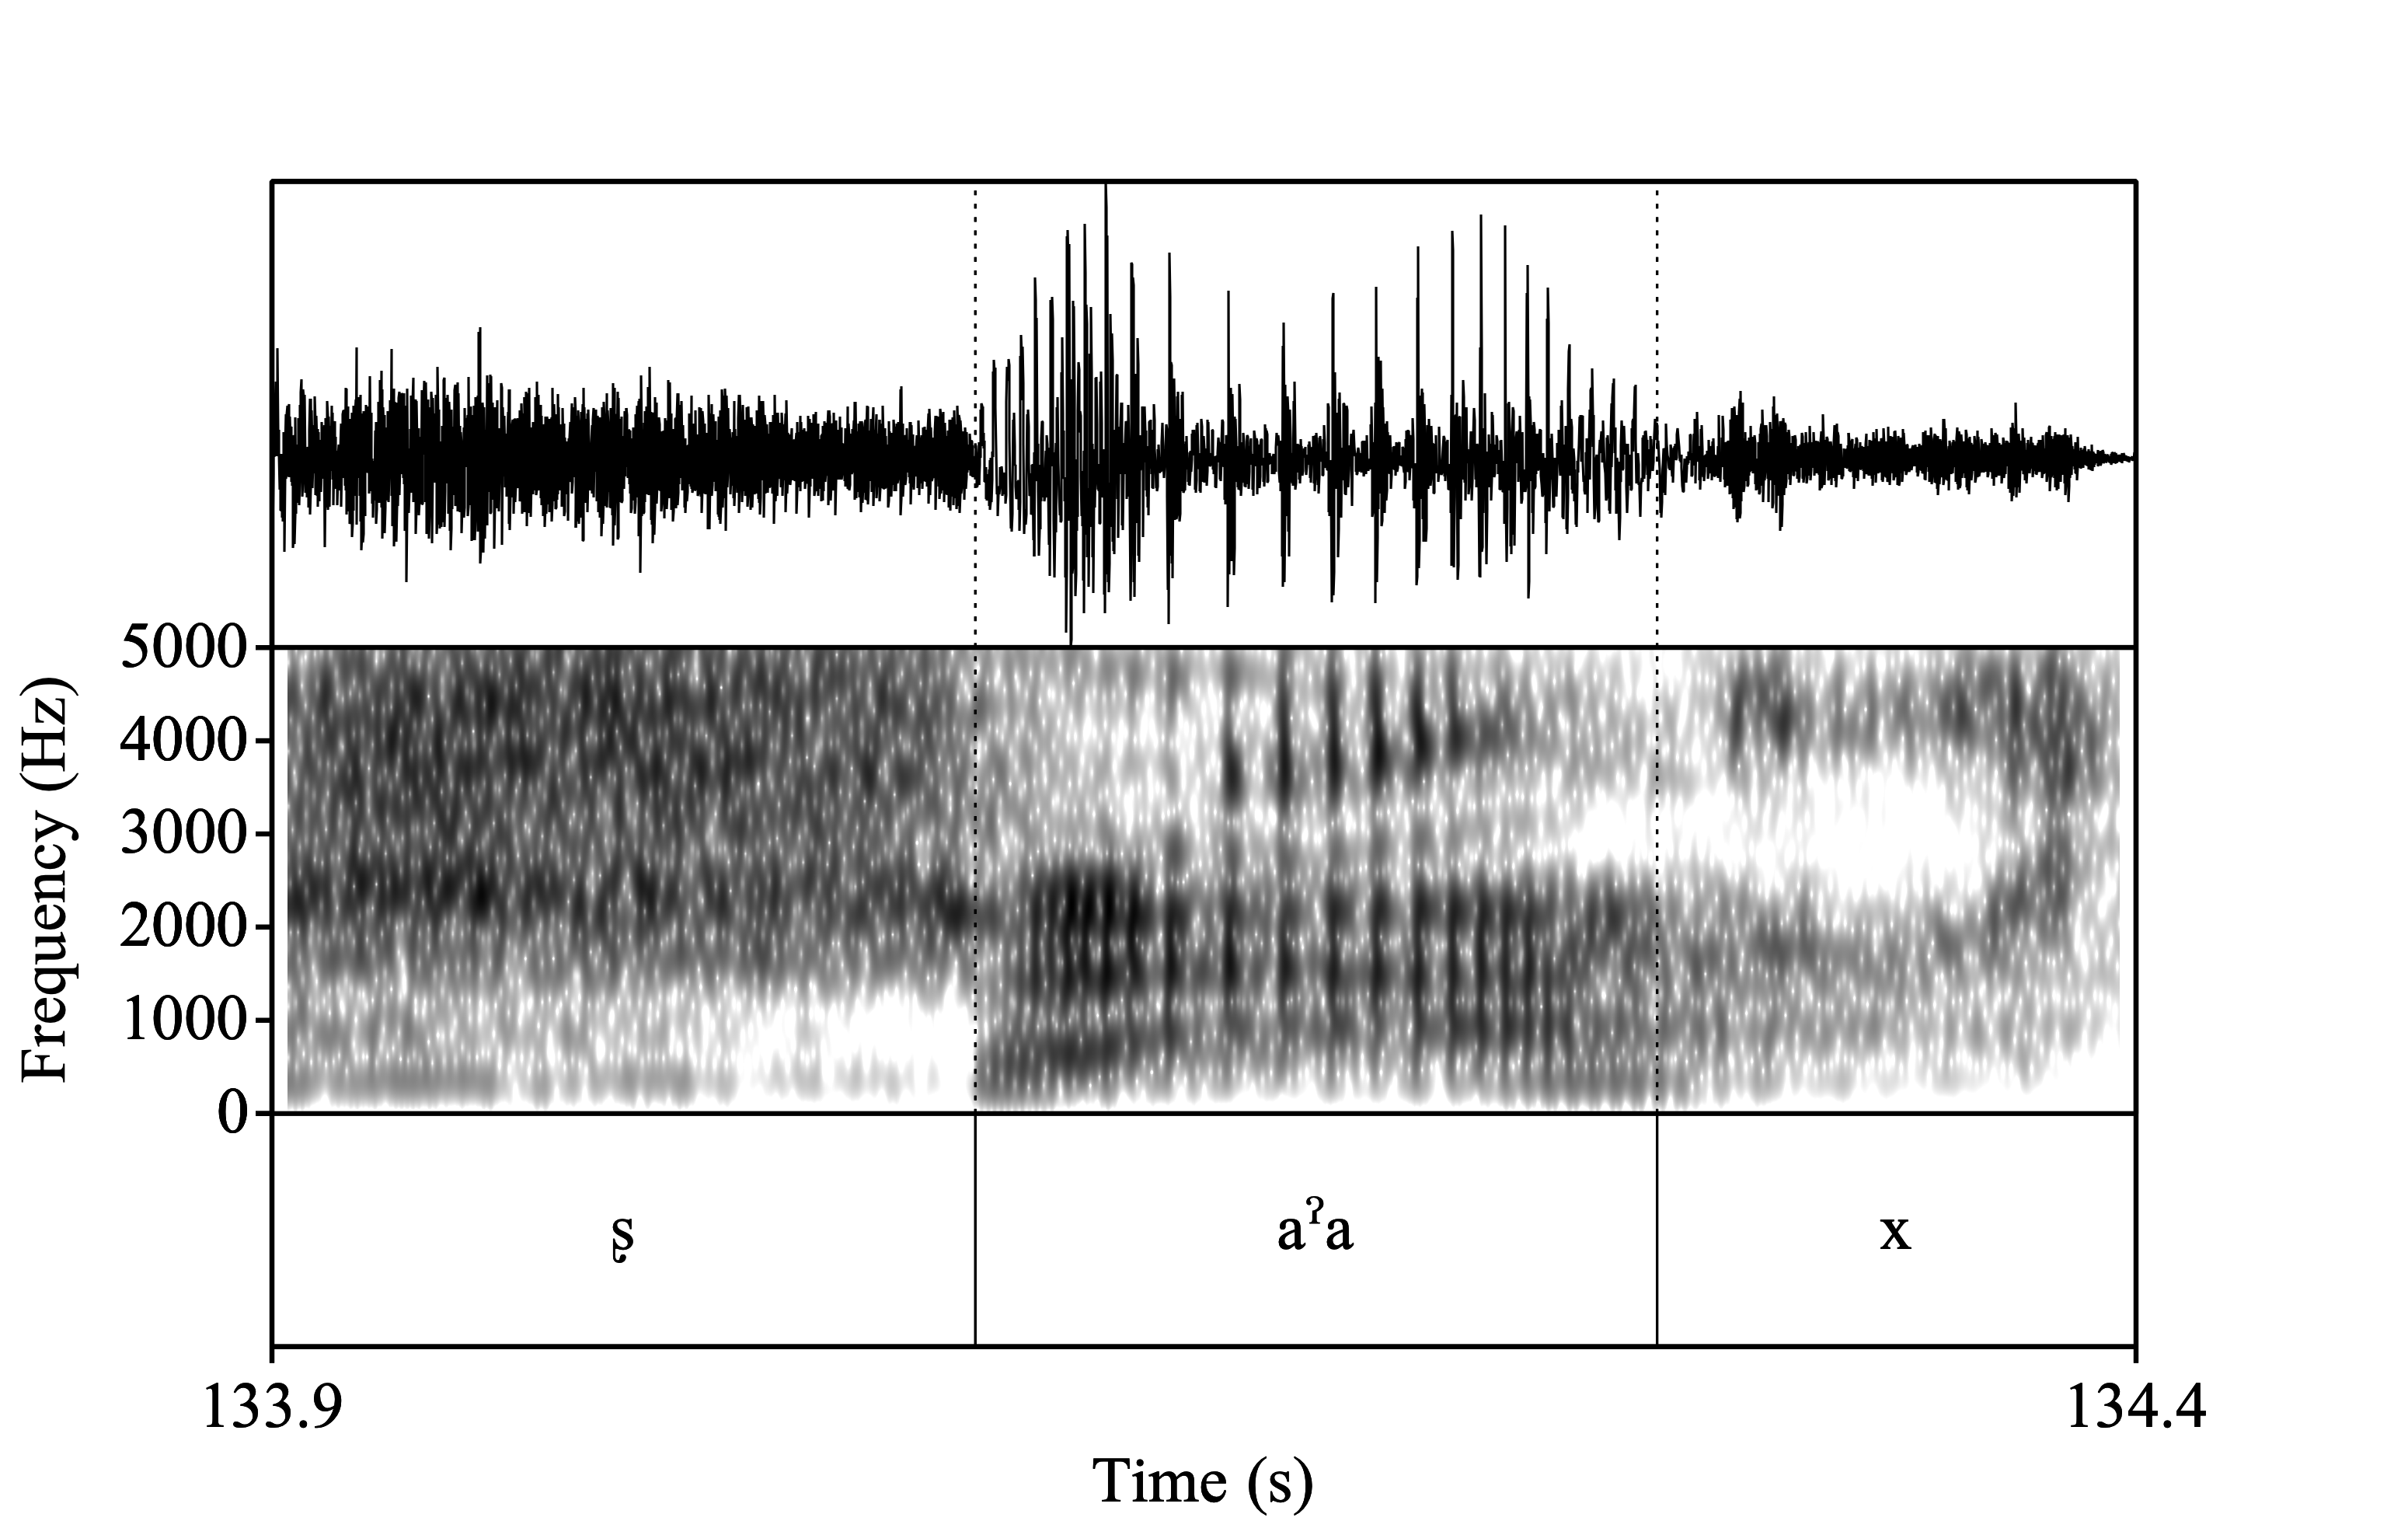
\includegraphics[width=\linewidth]{Images/xa'ag.png}
		\caption{\textit{xa'ag} `topil'}
		\label{fig:xa'ag}
	\end{subfigure}	
	\caption{Comparison of FSR's laryngealized vowels in \textit{za'a} `corncob' and \textit{xa'ag} `topil'}
	\label{fig:FSRLaryngeal}
\end{figure}

The other consultant only ever produces creaky voice for these vowels regardless of the tone of the word. During one of the elicitation sessions, we conducted a perceptual check that these were, in fact, the same vowels, and both consultants reliably identified the words and produced laryngealized vowels according to their own idiosyncrasies. However, a more detailed perception study is beyond the scope of this paper. 
\begin{figure}[!h]
	\centering
	\begin{subfigure}{.5\textwidth}
		\centering
		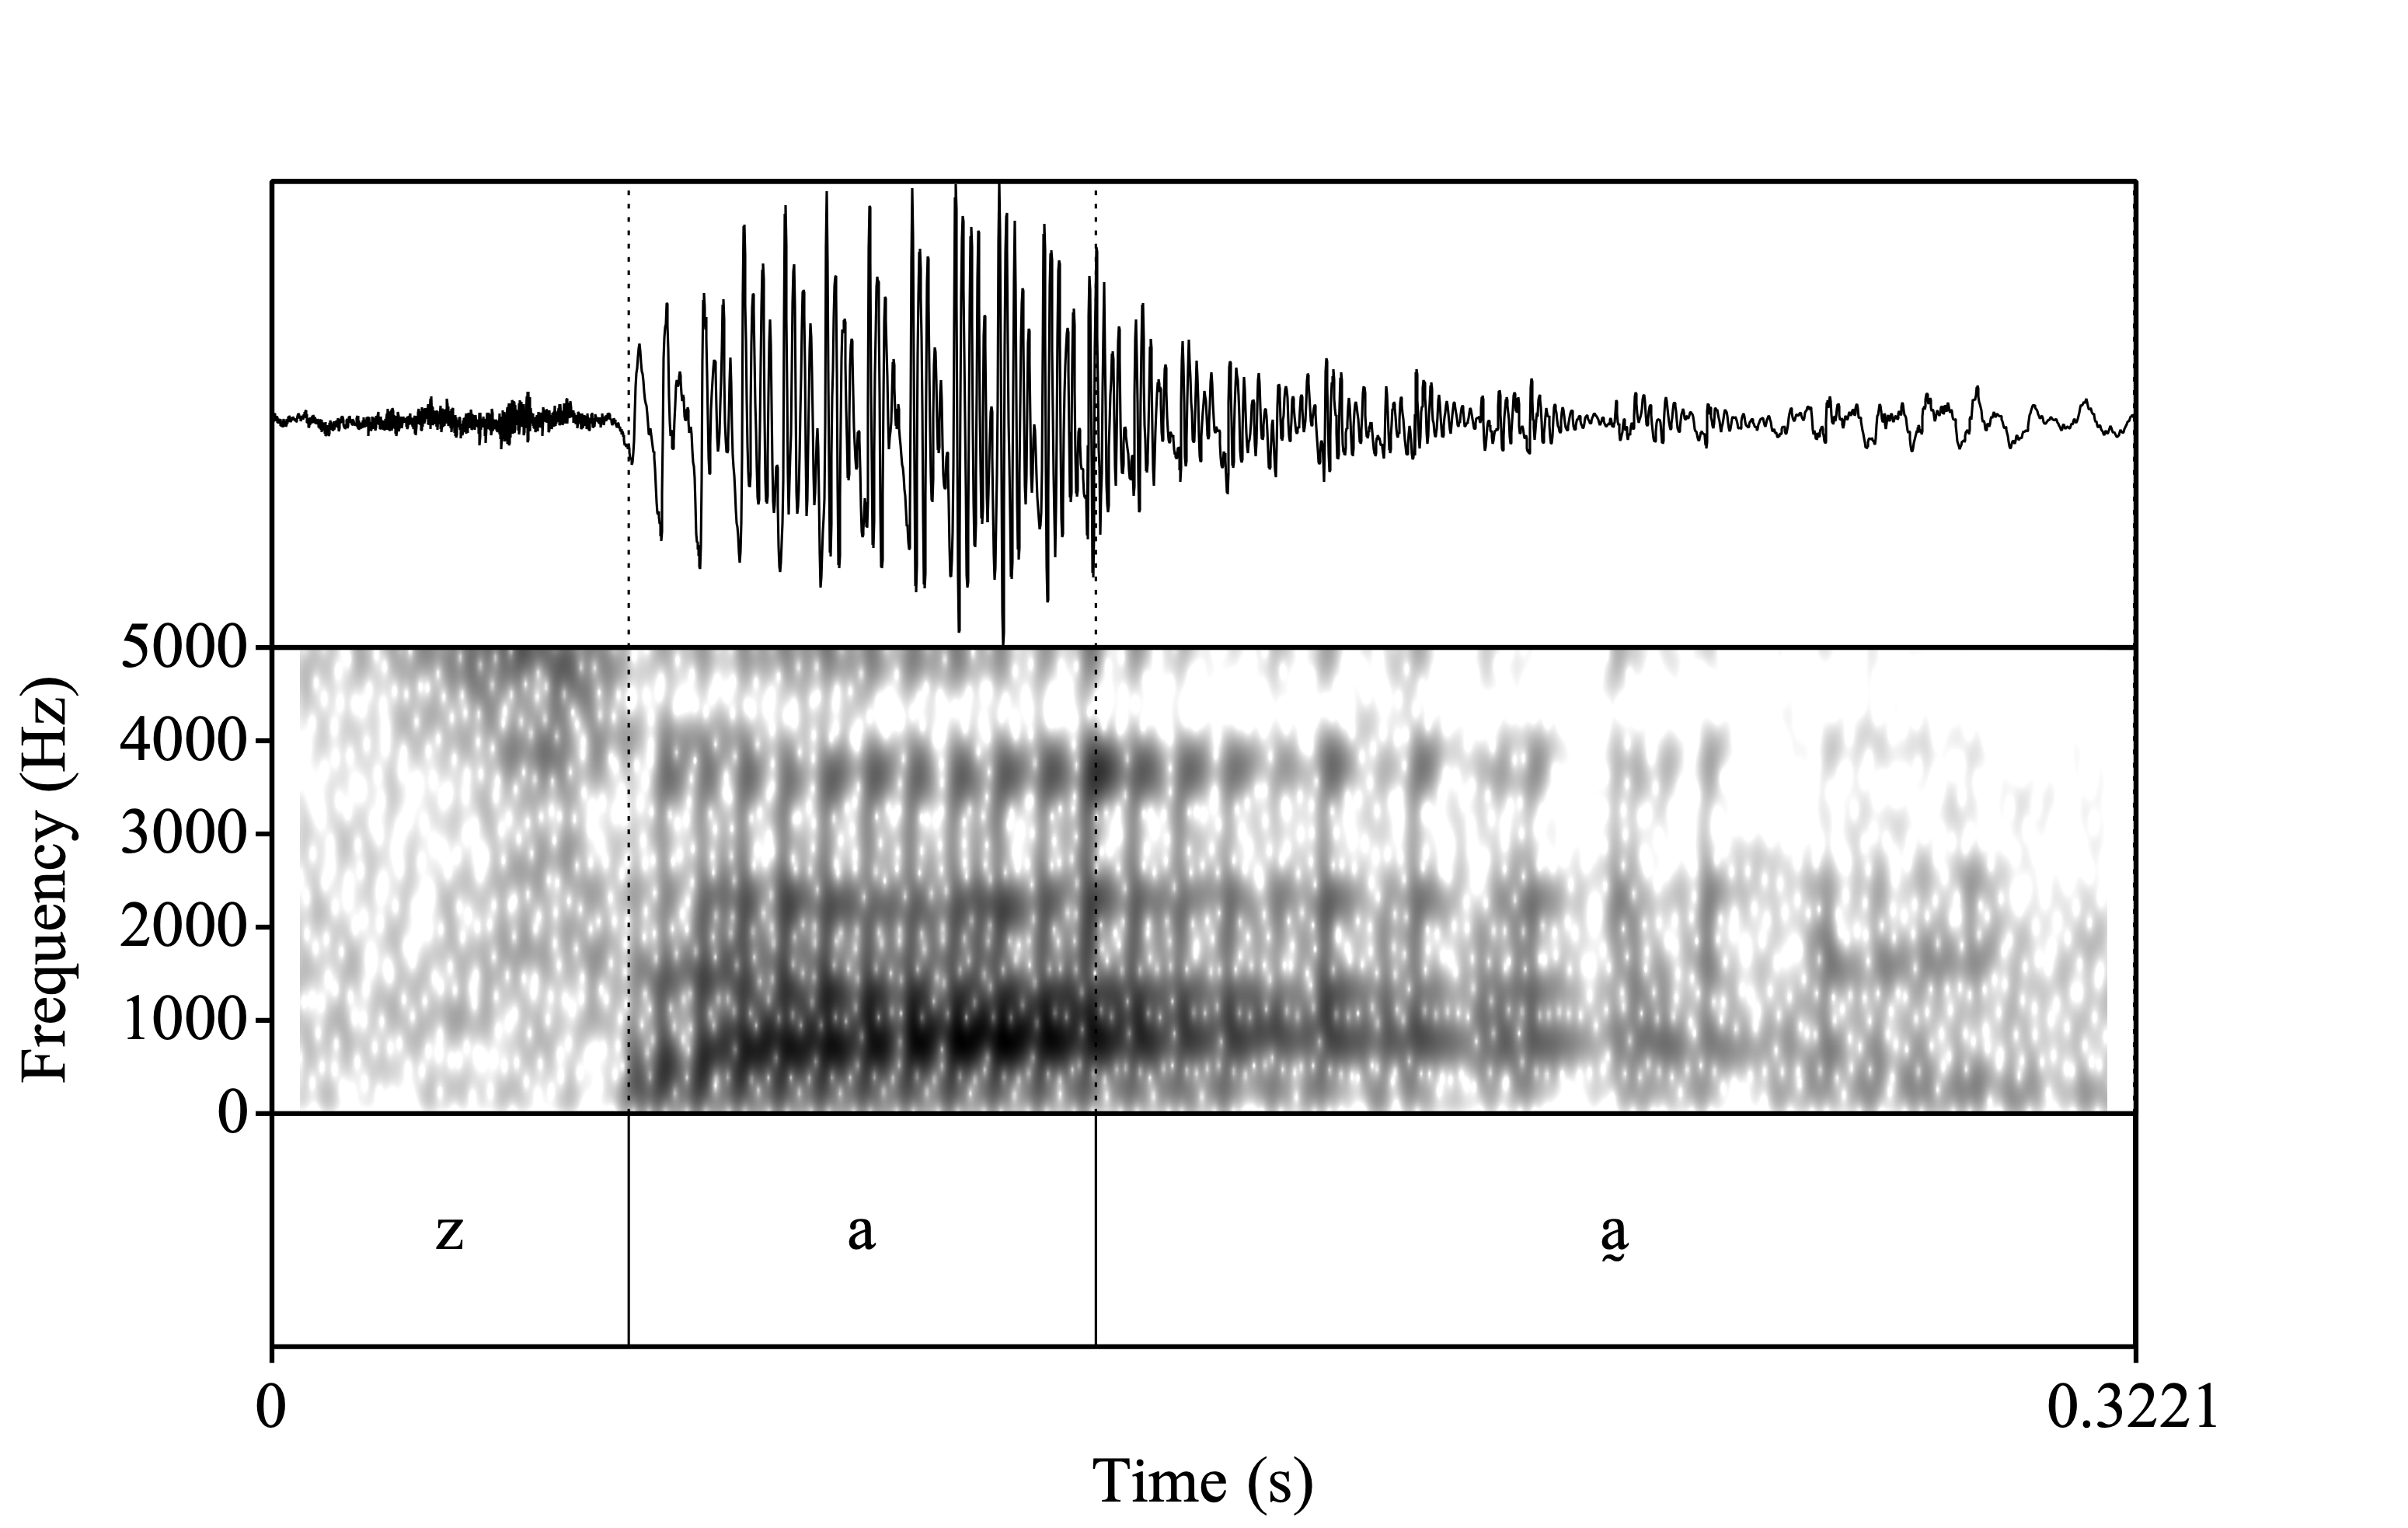
\includegraphics[width=\linewidth]{Images/RD_za'a.png}
		\caption{\textit{za'a} `corncob'}
		\label{fig:za'a}
	\end{subfigure}%
	\begin{subfigure}{.5\textwidth}
		\centering
		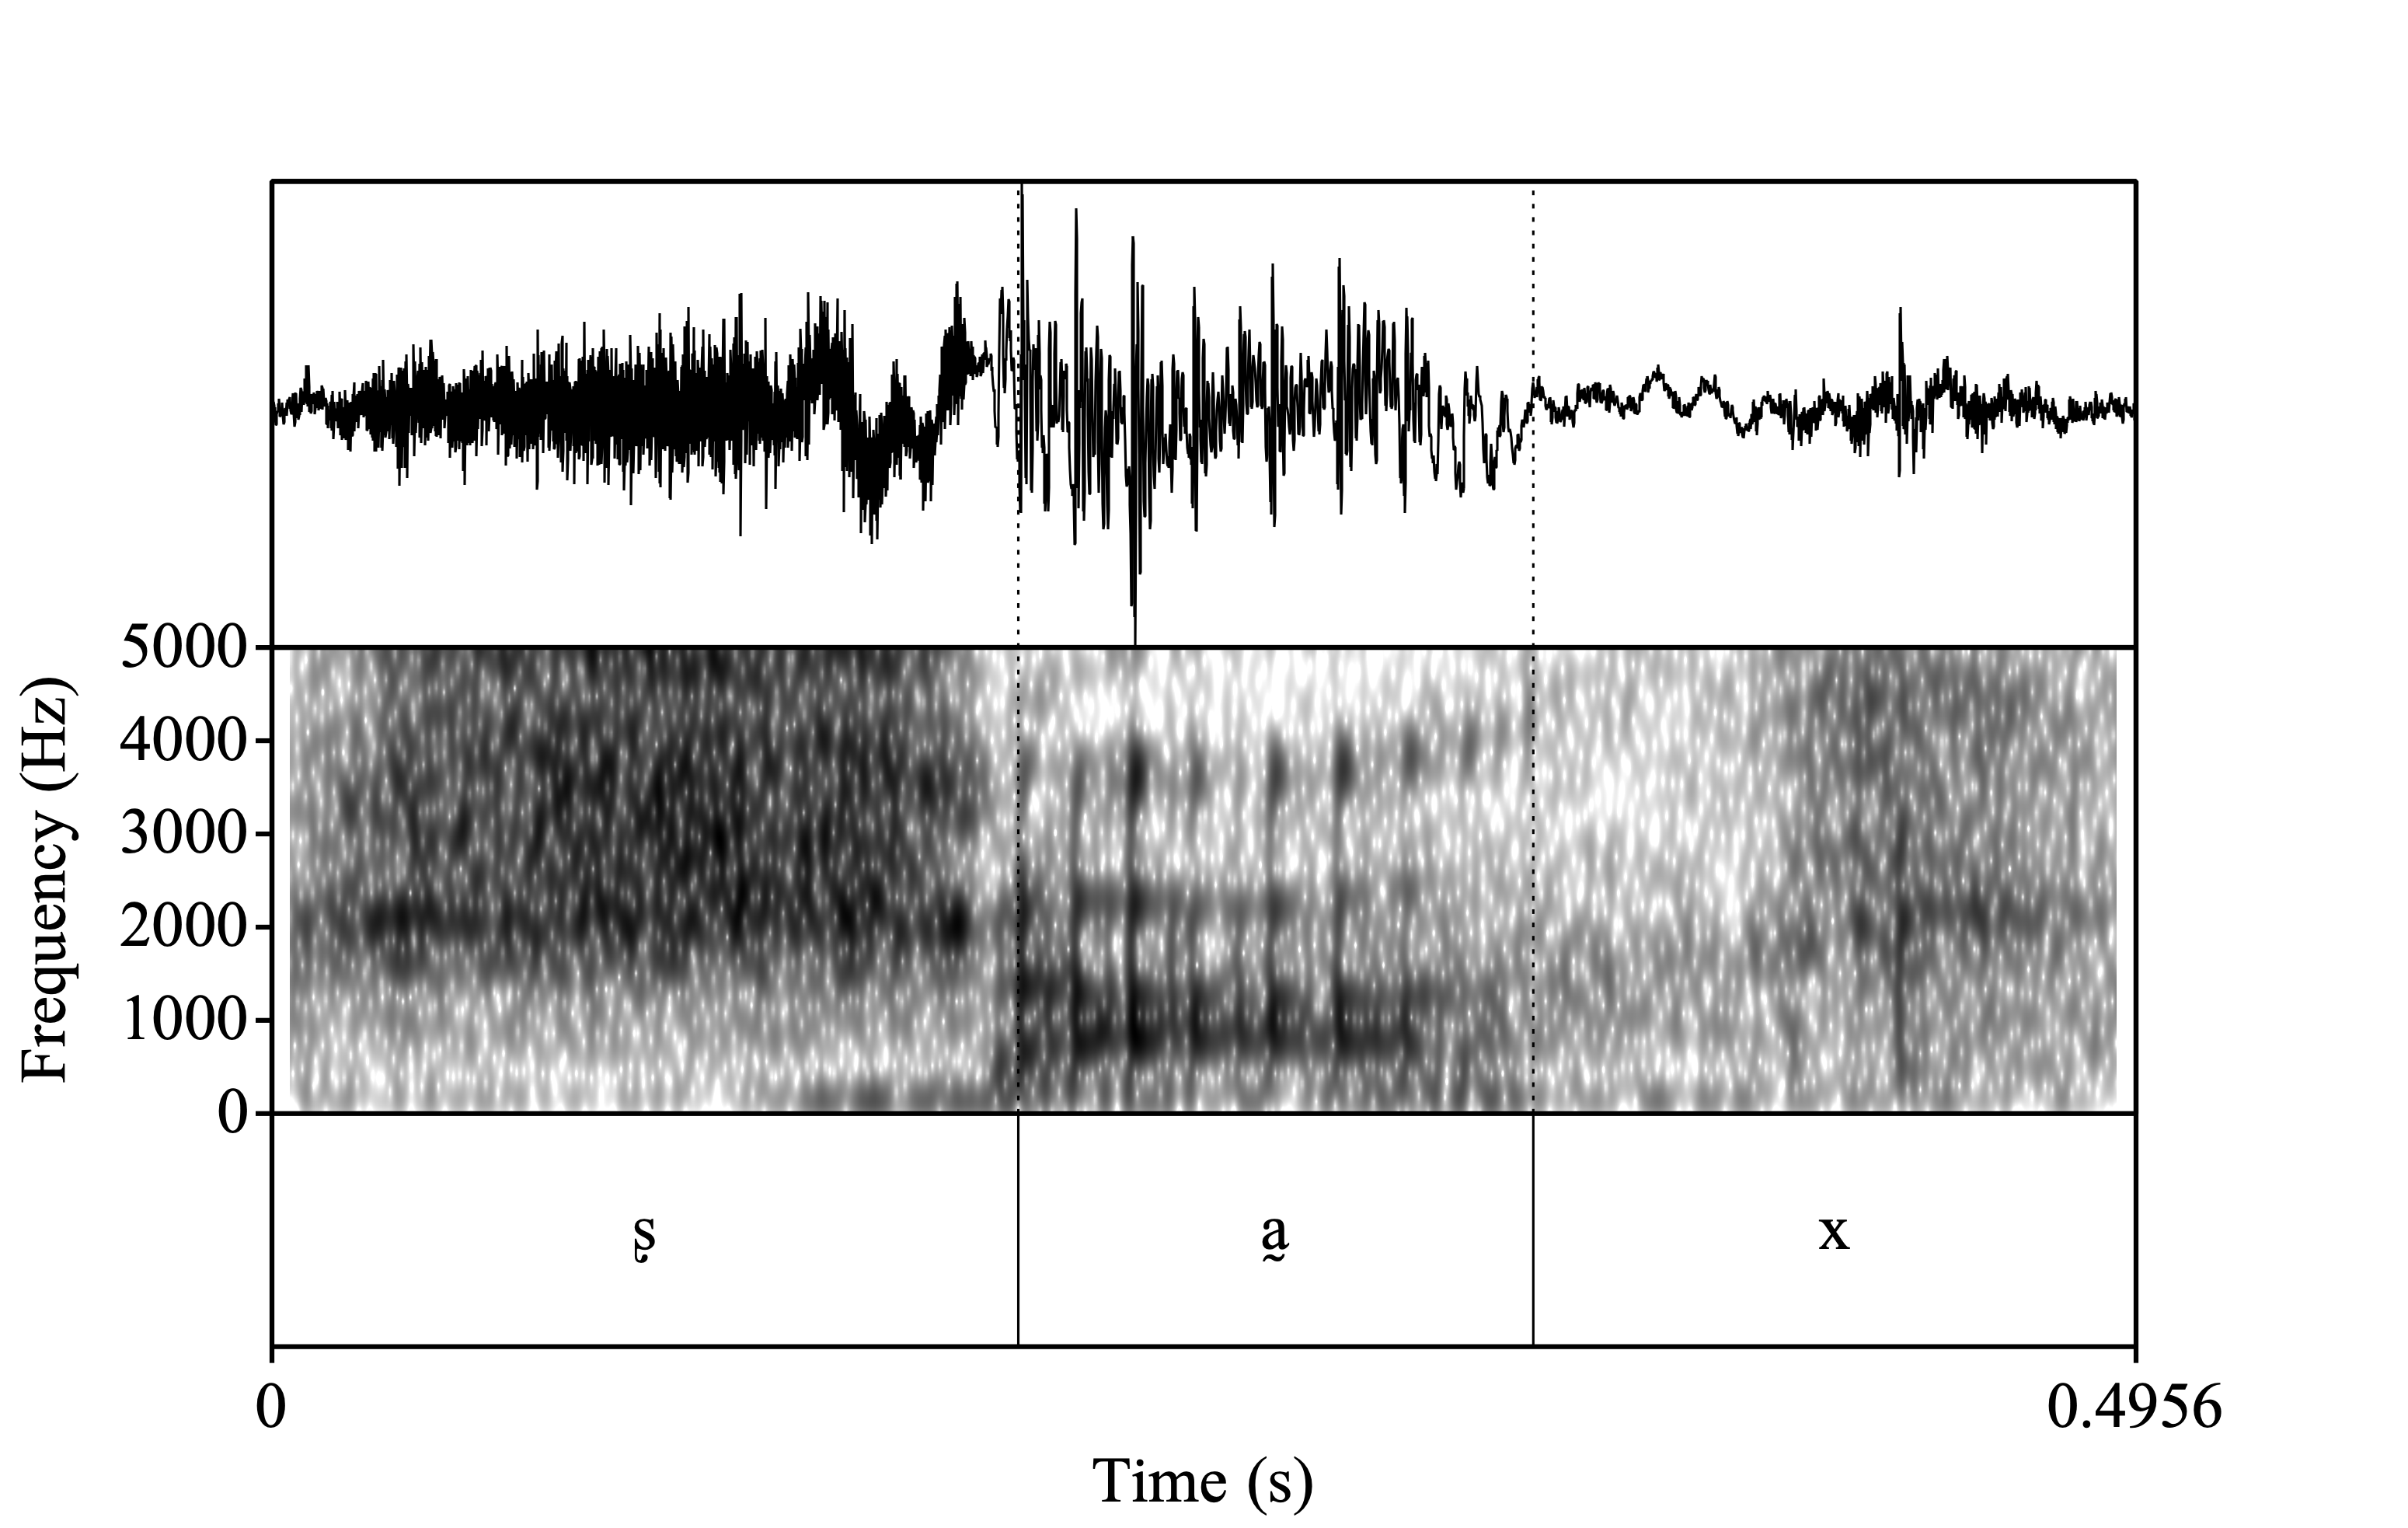
\includegraphics[width=\linewidth]{Images/RD_xa'ag.png}
		\caption{\textit{xa'ag} `topil'}
		\label{fig:xa'ag}
	\end{subfigure}
	\caption{Comparison of RD's laryngealized vowels in \textit{za'a} `corncob' and \textit{xa'ag} `topil'}
	\label{fig:RDLaryngeal}
\end{figure}

%------------------------------------
\subsection{Interaction of Tone and Phonation} \label{sec:Interaction}
%------------------------------------

Most previous work on the interaction of tone has been focused on the languages of East and Southeast Asia \citep[e.g.,][]{masicaDefiningLinguisticArea1976,thurgoodVietnameseTonogenesisRevising2002,yipTone2002,enfieldArealLinguisticsMainland2005,michaudComplexTonesEast2012,brunelleTonePhonationSoutheast2016}. What has been found in these descriptions is that certain tones and phonations are codependent. For example, \citet{smalleyProblemsConsonantsTone1976} and \citet{ratliffMeaningfulToneStudy1992} both describe White Hmong's \textit{-g} tone as being a mid-low tone with breathy phonation and Mandarin's tone 3 is often associated with creaky phonation \citep{hockettPeipingPhonology1947}. \citet{brunelleTonePerceptionNorthern2009} found that creaky phonation plays an important role in producing certain tones. Additionally, work on S'gaw Karen has found that two tones are only differentiated by the presence of some form of non-modal phonation (Boehm p.c.). 

However, there have been some observations–especially in Mesoamerica–that tone and phonation are independent of each other \citep[e.g,][]{silvermanLaryngealComplexityOtomanguean1997,garellekAcousticConsequencesPhonation2011}. This means that tone can independently occur with any phonation type. This has also been extensively described in multiple Zapotecan languages \citep[e.g.,][]{,avelinobecerraTopicsYalalagZapotec2004,avelinoAcousticElectroglottographicAnalyses2010, chavez-peonInteractionMetricalStructure2010, campbellZenzontepecChatinoAspect2011,villardPhonologyMorphologyZacatepec2015, lopeznicolasEstudiosFonologiaGramatica2016}

\citet{chavez-peonInteractionMetricalStructure2010} describes the tone and phonation interactions in San Lucas Quiaviní Zapotec (SLQZ), a central valley variety of Zapotec. The distribution of tone and phonation is found in Table~\ref{tab:SLQZ}. We see that in SLQZ, both low- and falling-tones have the full range of possible combinations. However, we see gaps in the high-tone for breathy and rising tones that can only occur with modal phonation. 

\begin{table}[!ht]
	\centering
	\caption{SLQZ tone and phonation interactions \citep{chavez-peonInteractionMetricalStructure2010}.}
	\label{tab:SLQZ}
	 \begin{tabular}{lcccc}
	  \lsptoprule
					  &	 \textbf{Modal}  & \textbf{Breathy} & \textbf{Creaky} & \textbf{Interrupted} \\
		  High	& ✔︎ & -- & ✔︎ & ✔︎ \\
		  Low & ✔︎ & ✔︎ & ✔︎ & ✔︎ \\
		  Falling & ✔︎ & ✔︎ & ✔︎ & ✔︎ \\
		  Rising & ✔︎ & -- & -- & -- \\
	  \lspbottomrule
	 \end{tabular}
\end{table}

Based on elicitation data collected from 2020-2022, SLZ has a more expansive distribution of tone and phonation when compared to SLQZ but seems to be very similar to other Northern Zapotec varieties \citep[e.g.,][]{avelinobecerraTopicsYalalagZapotec2004}. The distribution of SLZ tonal and phonation interactions are given in Table~\ref{tab:ToneVoiceQuality} for the number of tokens that were analyzed. 
\begin{table}[!h]
	\caption{SLZ tone and phonation interactions.}
	\label{tab:ToneVoiceQuality}
	\centering

	\begin{tabular}{lcccc}
	\lsptoprule
		& \textbf{Modal} & \textbf{Breathy} & \textbf{Checked} & \textbf{Laryngealized} \\
	\hline
	High		& ✔︎ & -- & ✔︎ & ✔︎ \\
	Mid			& ✔︎ & ✔︎ & ✔︎ & ✔︎ \\
	Low			& ✔︎ & ✔︎ & ✔︎ & ✔︎ \\
	High-Low	& ✔︎ & ✔︎ & ✔︎ & ✔︎ \\
	Mid-High	& ✔︎	& ✔︎ & -- & ✔︎ \\
	\lspbottomrule
	\end{tabular}
\end{table}

One of the striking things in this is the lack of high tone with breathy phonation. This gap is interesting because of the long-time association of high pitch with breathiness \citep[a good overview–of this association and other phonation types–is found in][]{eslingVoiceQualityLaryngeal2019}. This breathy phonation and high tone gap are quite common across the Zapotecan languages (Campbell p.c.). Regarding breathy phonation in SLQZ, \citet{uchiharaToneRegistrogenesisQuiavini2016} offers some convincing evidence that the phonation originated in syllables with low tone and then spread to other tones via analogy. If this is also true for SLZ, then we should be able to find similar distributions that Uchihara observes when we compare SLZ to its closest relative, San Bartolomé Zoogocho Zapotec, which lacks a breathy phonation. Such an investigation would be important in understanding how breathy vowels originated in the Zapotecan family, but is beyond the scope of this paper.  

 

%------------------------------------
\section{Methodology} \label{sec:Methods}
%------------------------------------

Due to the impact of the COVID-19 pandemic, only two native language speakers of SLZ were able to take part in this study (one male; one female). Both speakers live in Santa Cruz, CA. The data collection was done remotely using Zencastr\footnote{\href{https://zencastr.com/}{https://zencastr.com/}}, a professional podcasting website (44.1kHz, 16-bit) or in-person outside in a well-ventilated location, using a Zoom H4n handheld recorder (44.1kHz, 16-bit). Participants were recorded saying approximately 100 words in the carrier sentence \textit{shnia' X chone las} `I say X three times'. This phrase was repeated three times. 

After the elicitations were completed, the audio was uploaded into ELAN \citep{wittenburgELANProfessionalFramework2006} for initial segmentation into sentences. This was followed by segmenting the target vowels in Praat \citep{boersmaPraatDoingPhonetics2021}. These segments were then fed into VoiceSauce \citep{shueVOICESAUCEProgramVoice2009}, where each vowel was resampled at 16kHZ for acoustic measurement. The acoustic measurements of VoiceSauce were then analyzed in R \citep{rcoreteamLanguageEnvironmentStatistical2021}. In order to investigate the effects of phonation on different portions of the vowel, each vowel was normalized for time, and following \citet{garellekAcousticConsequencesPhonation2011}, the resulting measurements were averaged for each third of the vowel. 

%------------------------------------
\section{Results of the acoustic analysis} \label{sec:Results}
%------------------------------------

In plotting the spectral-tilt measurements, we find that the results follow some of the established patterns and deviate in others. This section will first discuss the results of the H1-H2 measurements for both FSR and RD, the H1-A3 measurements for FSR and RD, and the CPP measurements for FSR and RD. 

%------------------------------------
\subsection{H1-H2 results} \label{sec:H1H2}
%------------------------------------

The clearest result that was gleaned from the H1-H2 measurements shows that the breathy voice is much lower than the measurement for modal vowels throughout much of the vowel. This can be seen in Figures~\ref{fig:FSRh1h2first}, \ref{fig:h1h2second}, and \ref{fig:h1h2third}. This behavior, however, is at odds with the observed patterns that breathy voice should have a higher H1-H2 value than the model's value. This suggests that instead of breathy voice is actually creaky. However, the correct behavior for breathy voice is observed in H1-A3; see Section~\ref{sec:H1A3}

\begin{figure}[!ht]
	\centering
	\begin{subfigure}{.5\textwidth}
		\centering
		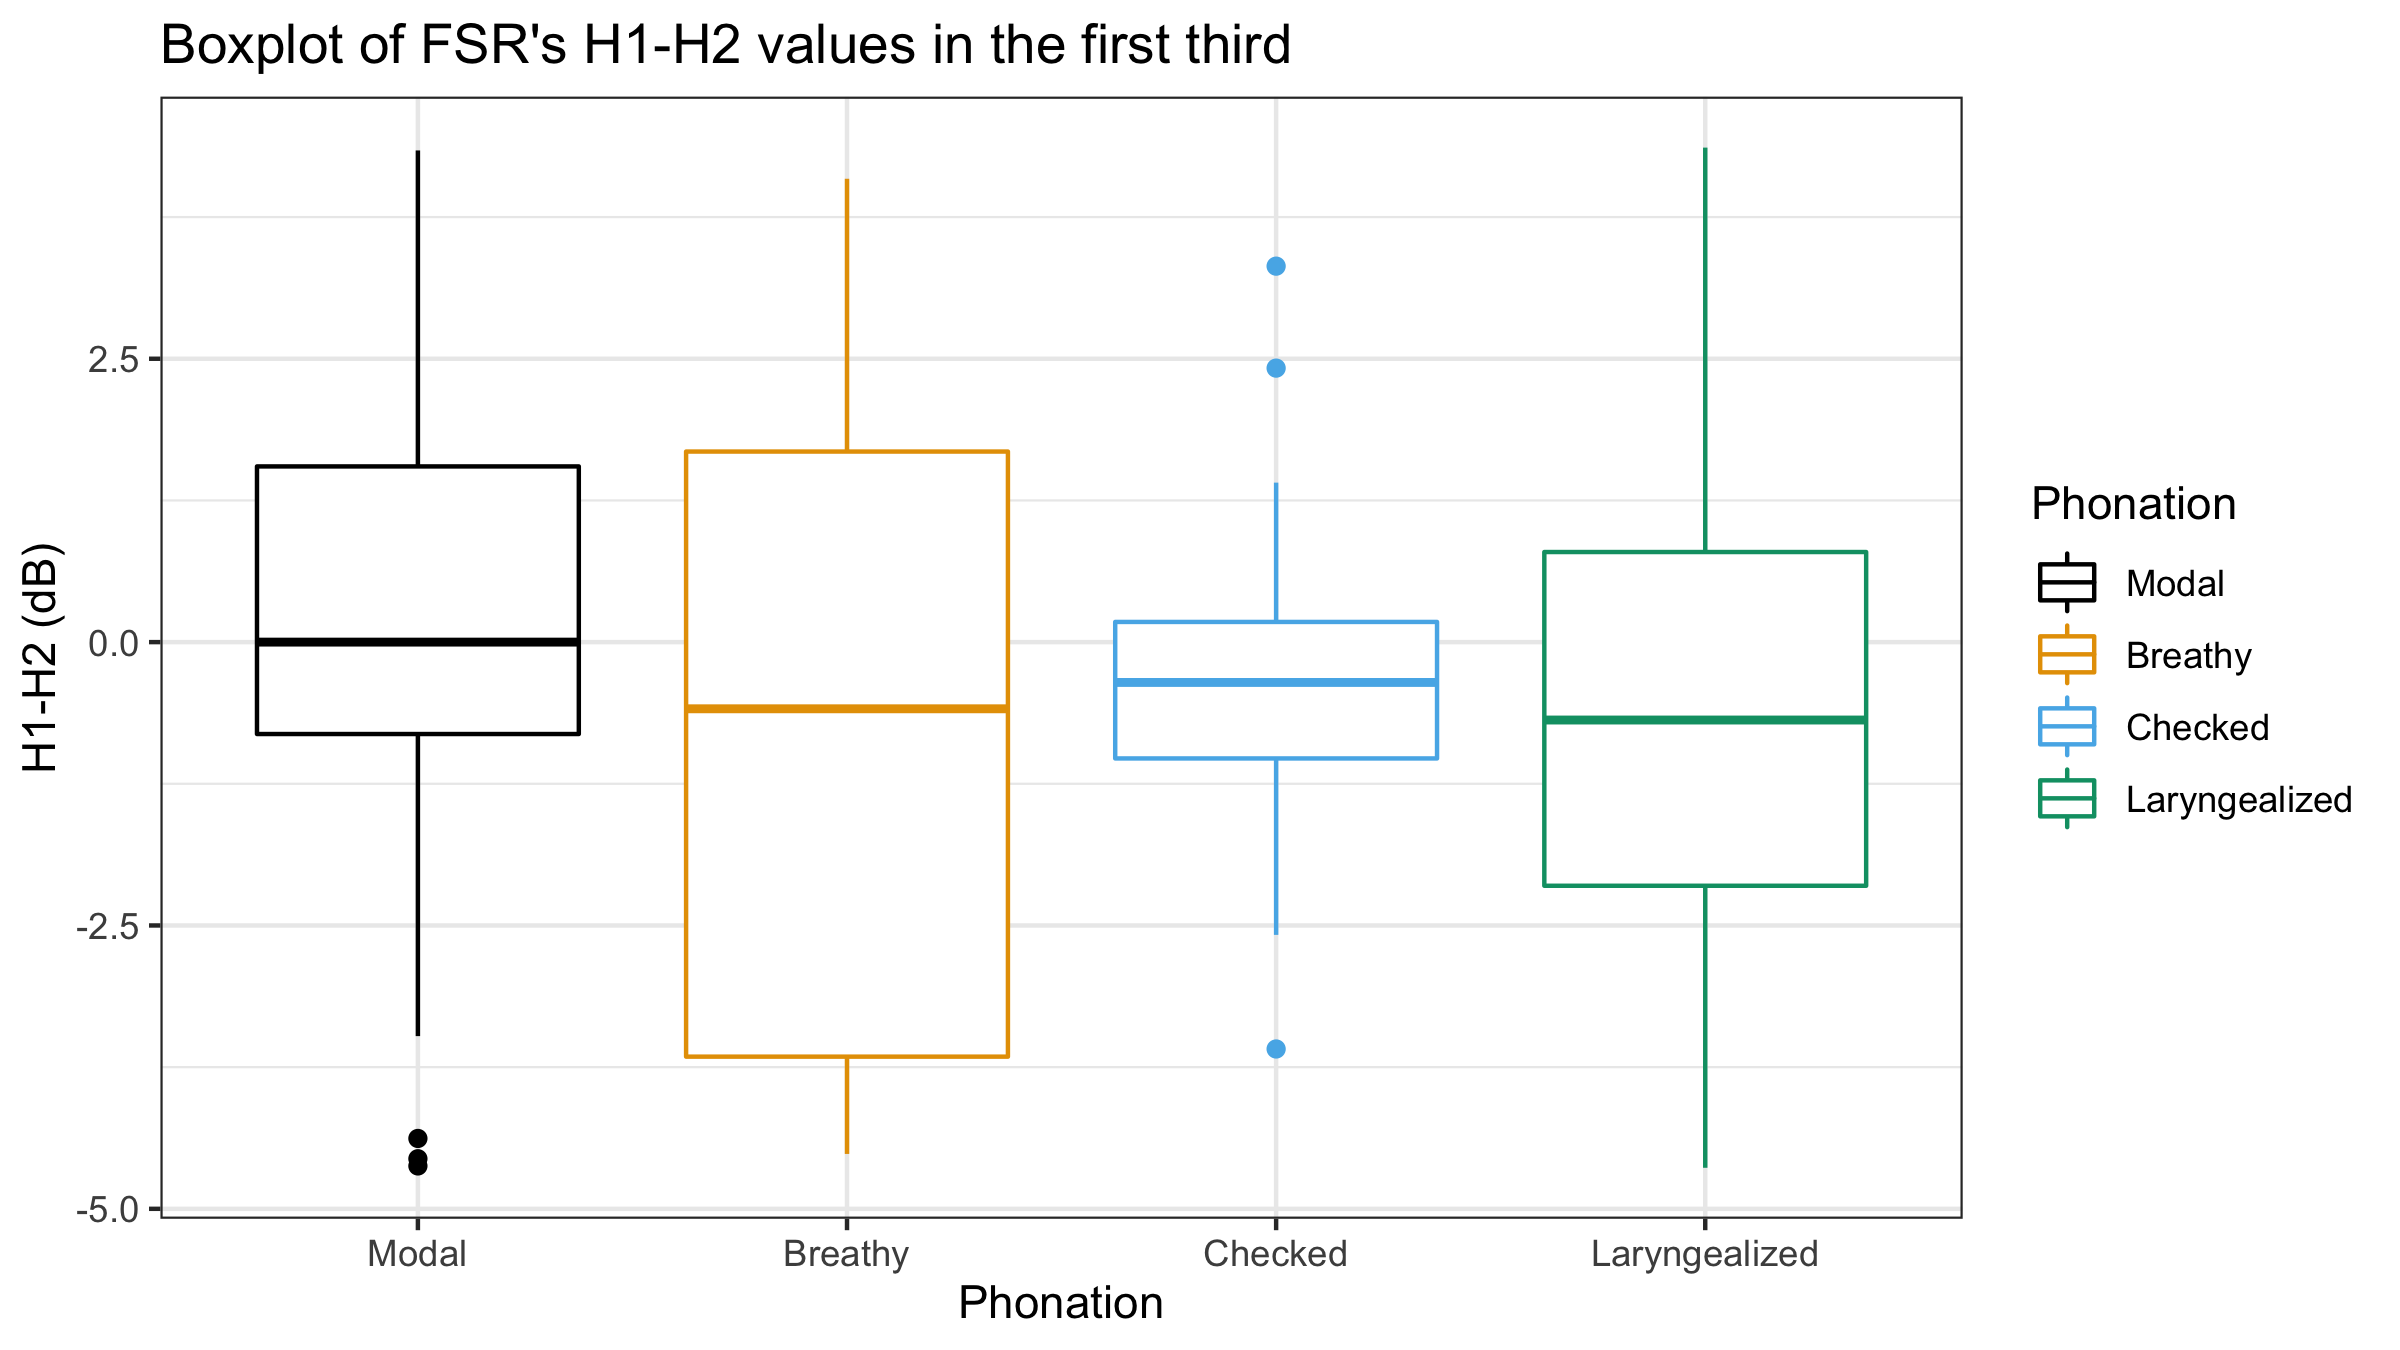
\includegraphics[width=0.9\textwidth]{Images/mean_FSR_h1h2_1st.png}
		\caption{FSR's H1-H2 values.}
		\label{fig:FSRh1h2first} 
	\end{subfigure}%
	\begin{subfigure}{.5\textwidth}
		\centering
		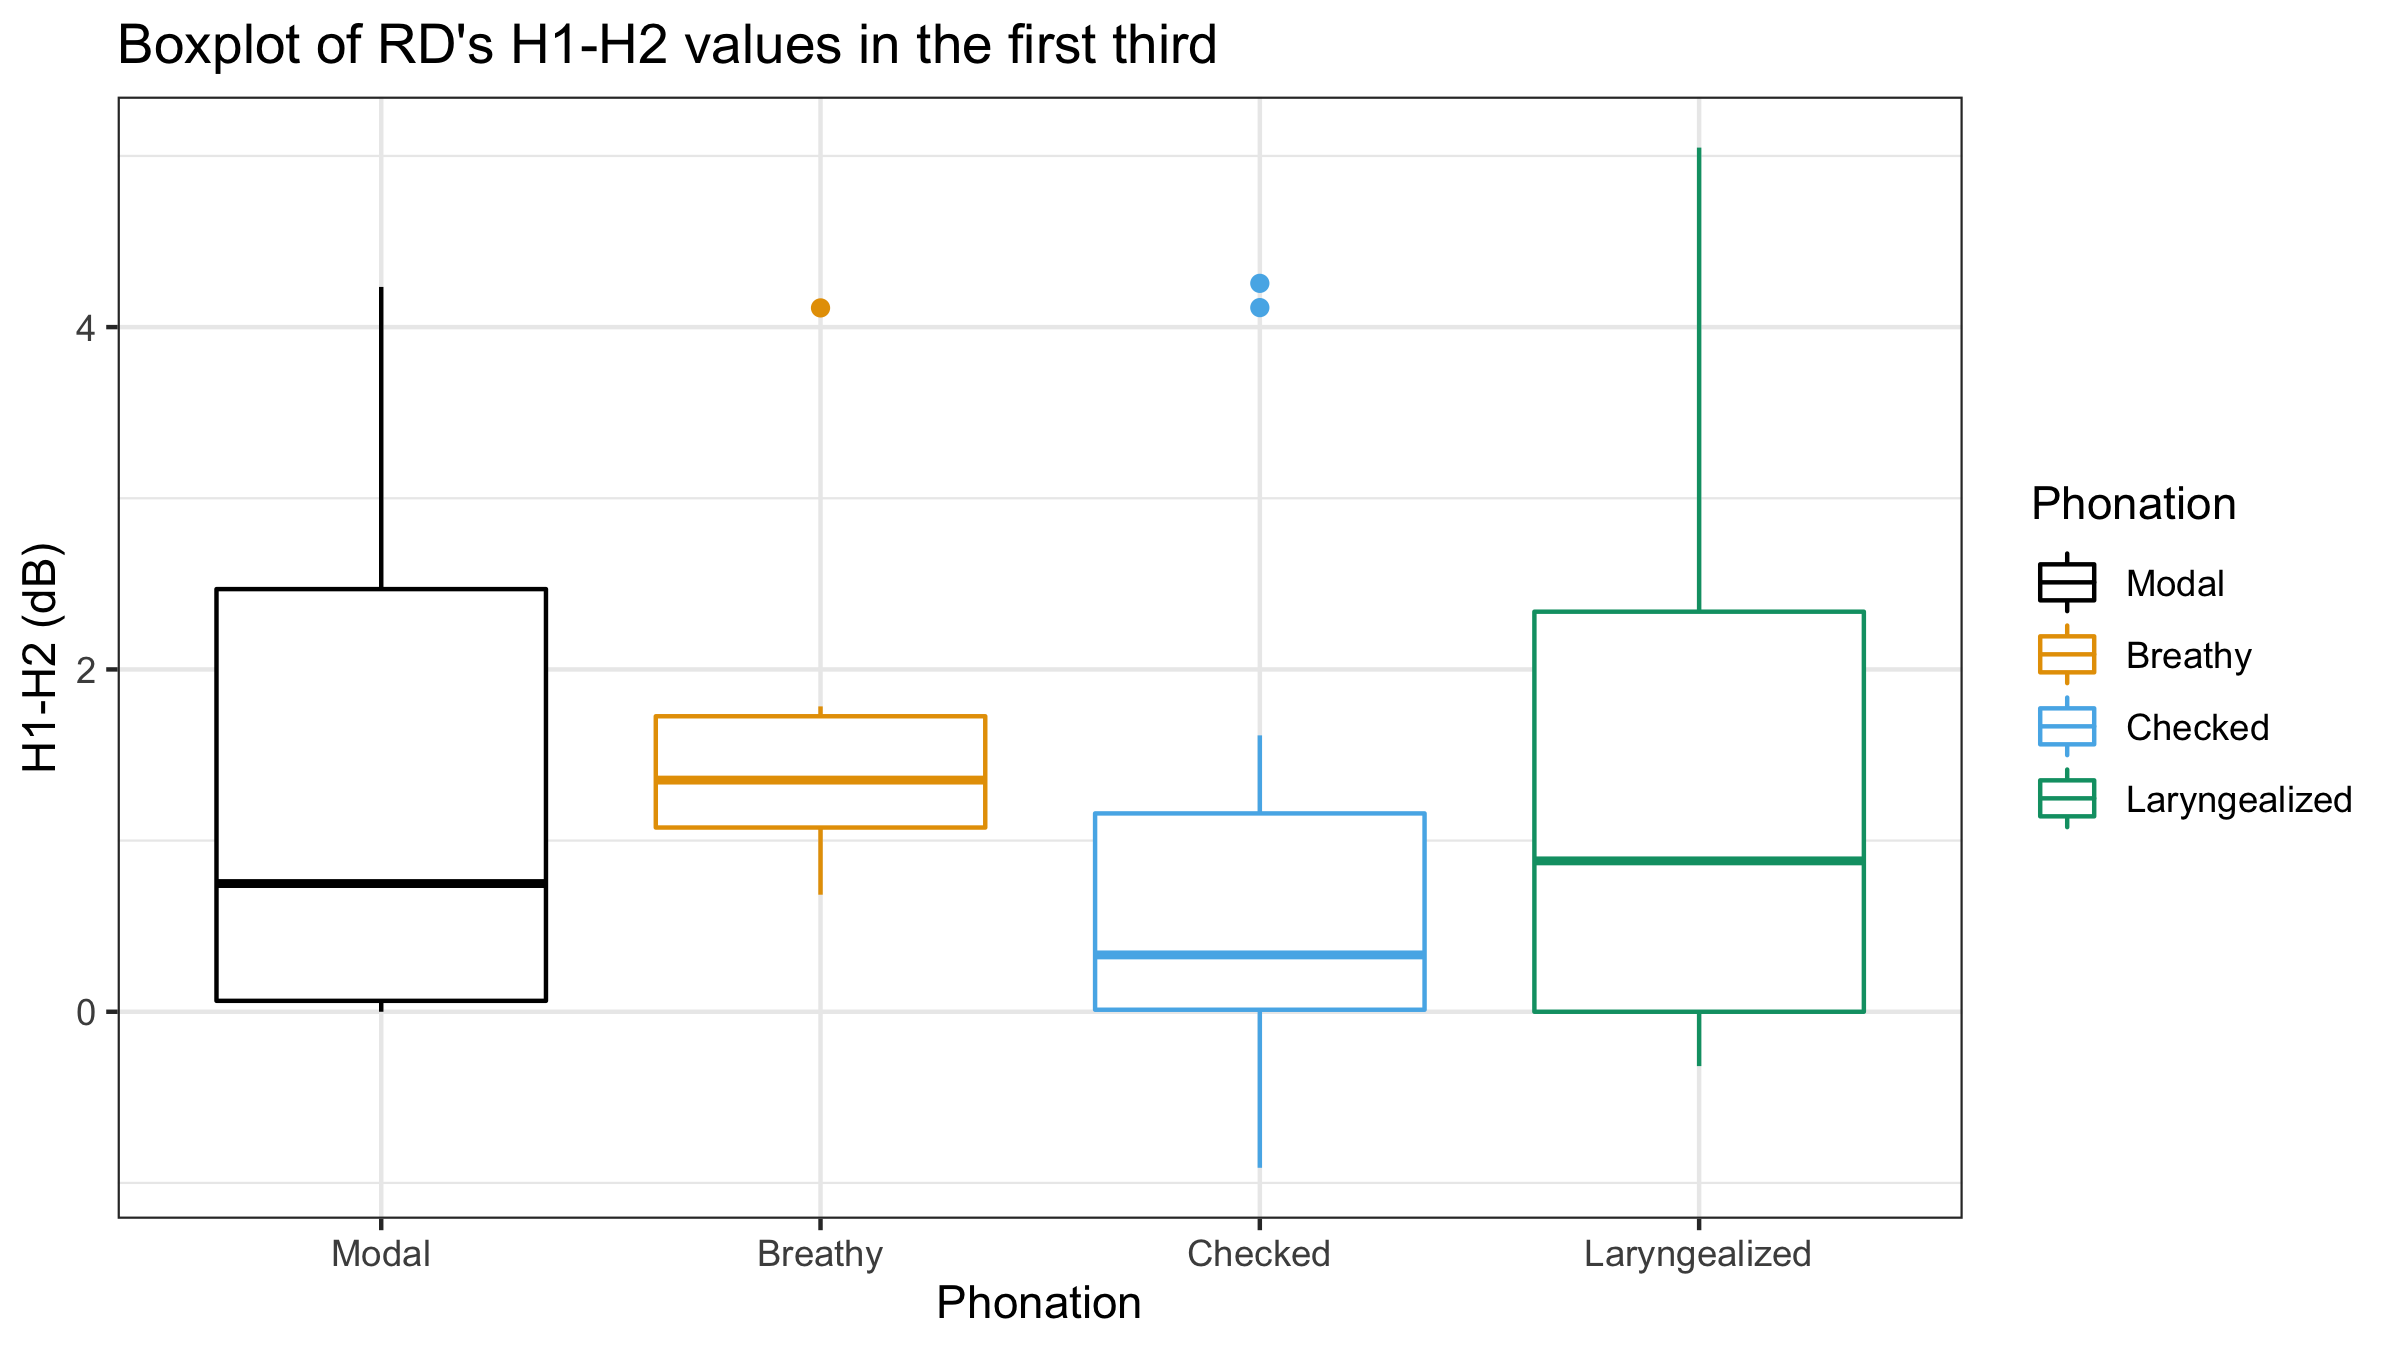
\includegraphics[width=0.9\textwidth]{Images/mean_RD_h1h2_1st.png}
		\caption{RD's H1-H2 values.}
		\label{fig:RDh1h2first} 
	\end{subfigure}
	\caption{Mean H1-H2 values for the first third of the vowel according to each phonation type. }
	\label{fig:h1h2first}
\end{figure}

Additionally, in the first third of the vowel, as shown in Figure~\ref{fig:h1h2first}, we see that the mean values for checked vowels are lower than those for modal vowels. This is true for both FSR and RD. In regards to laryngealized vowels, the mean value for H1-H2 is nearly identical to that for modal vowels for RD. However, for FSR the value is lower.

\begin{figure}[!ht]
	\centering
	\begin{subfigure}{.5\textwidth}
		\centering
		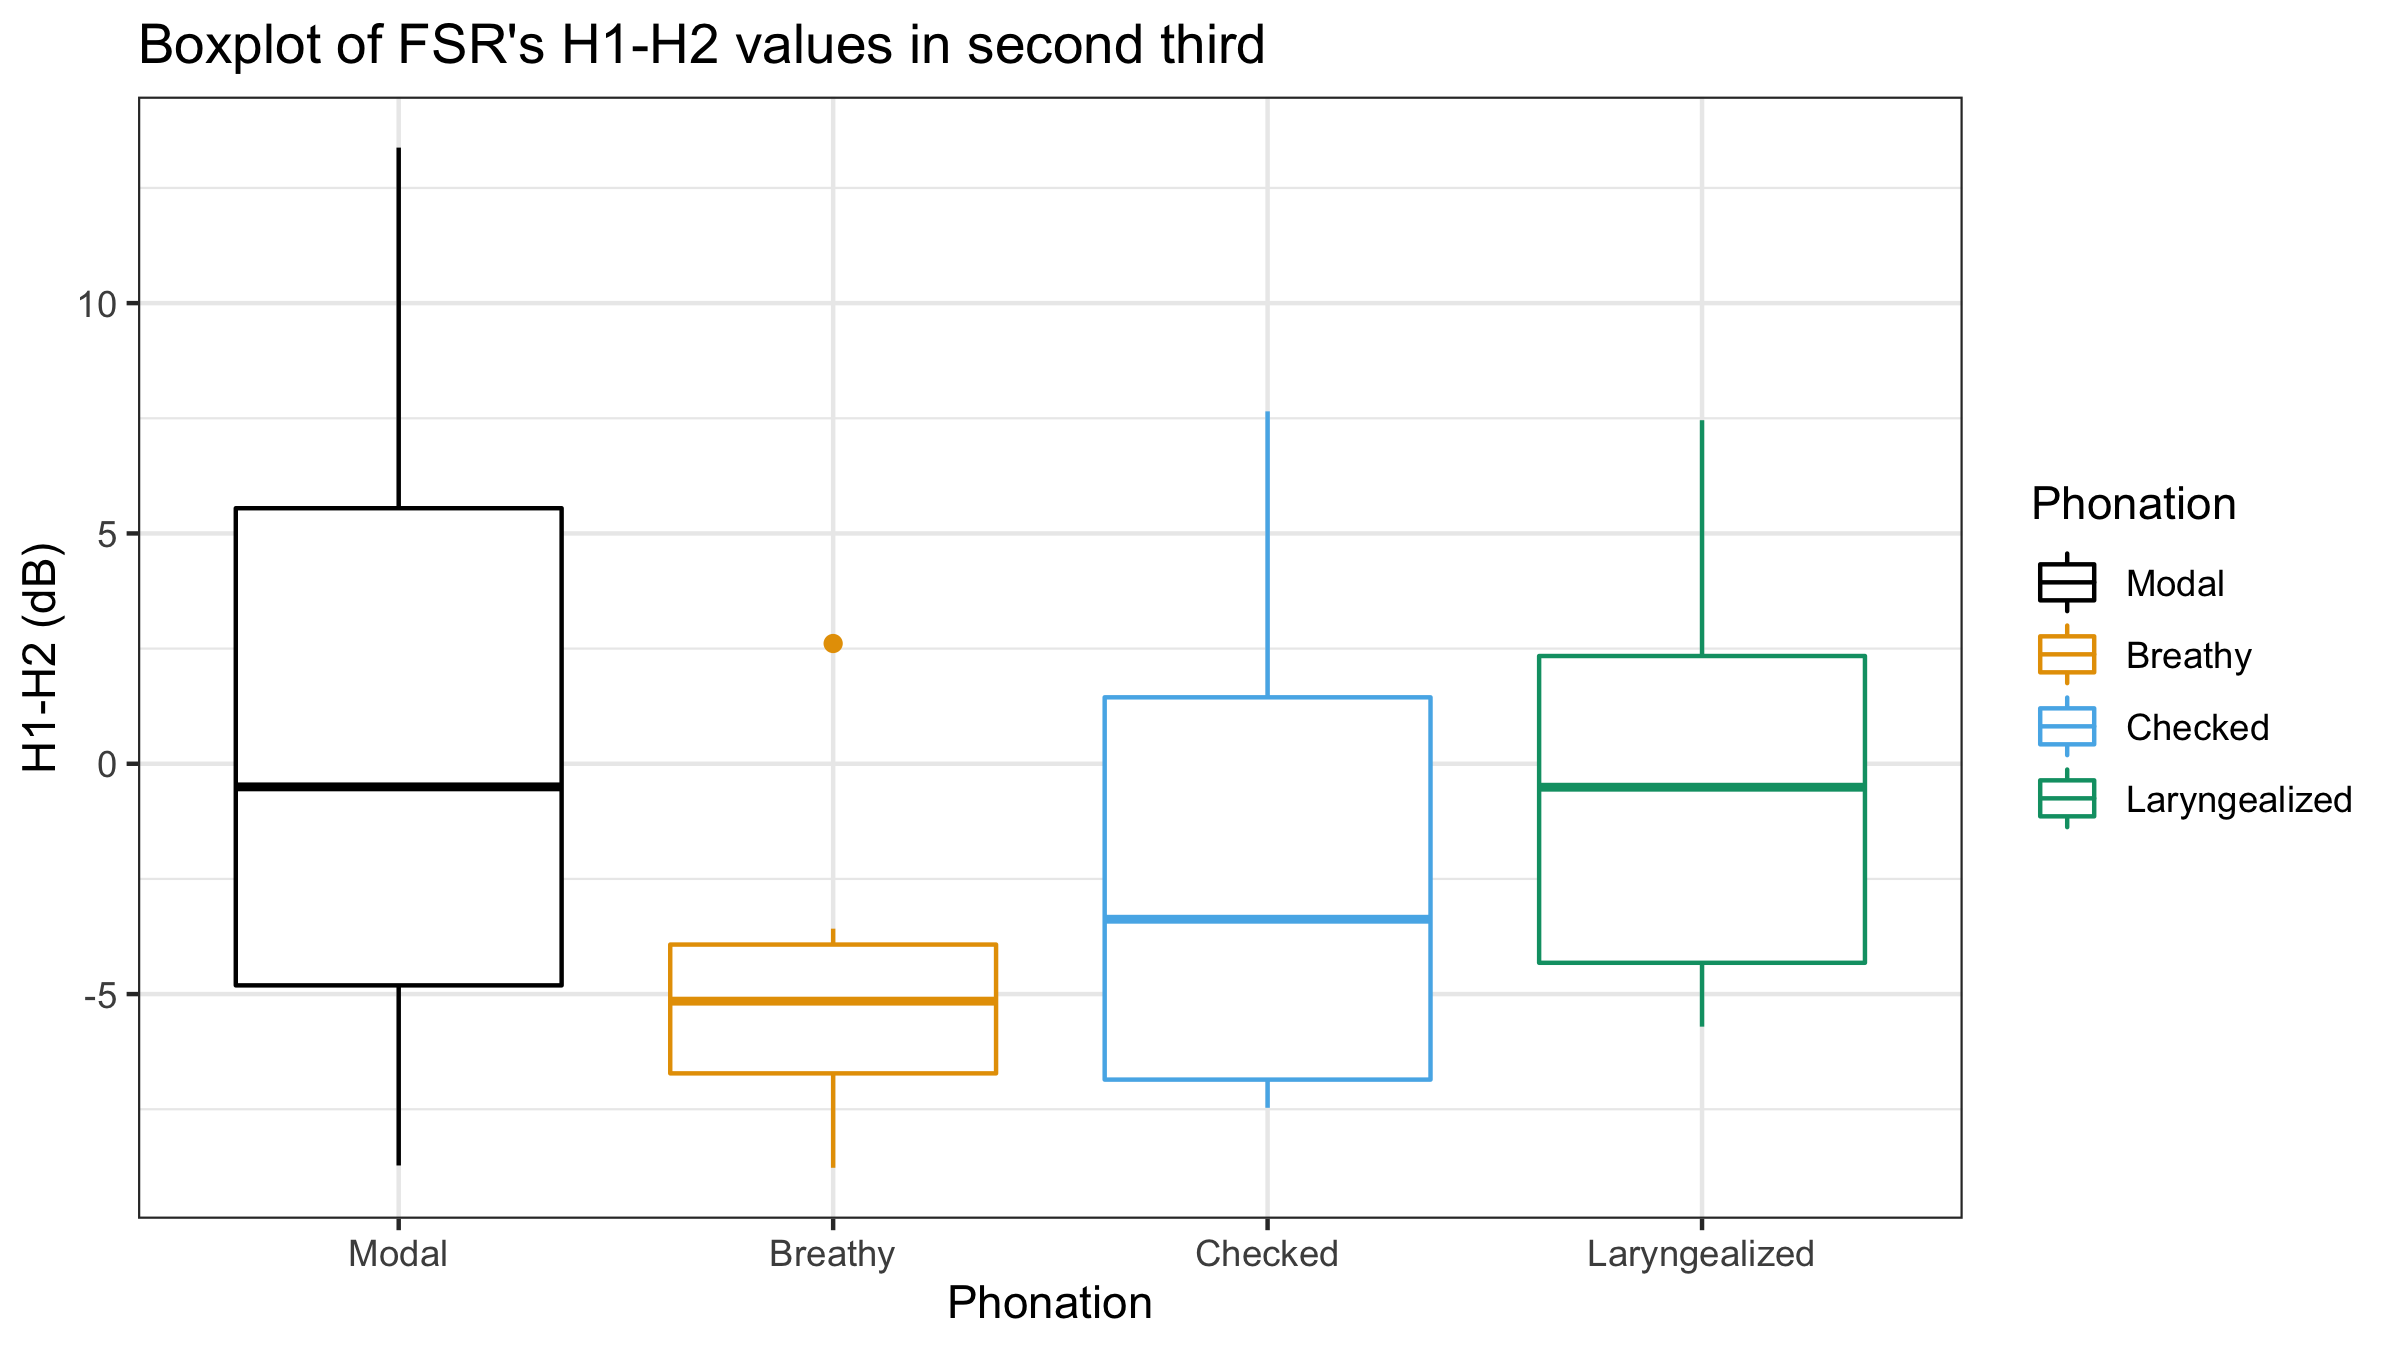
\includegraphics[width=0.9\textwidth]{Images/mean_FSR_h1h2_2nd.png}
		\caption{FSR's H1-H2 values.}
		\label{fig:FSRh1h2second} 
	\end{subfigure}%
	\begin{subfigure}{.5\textwidth}
		\centering
		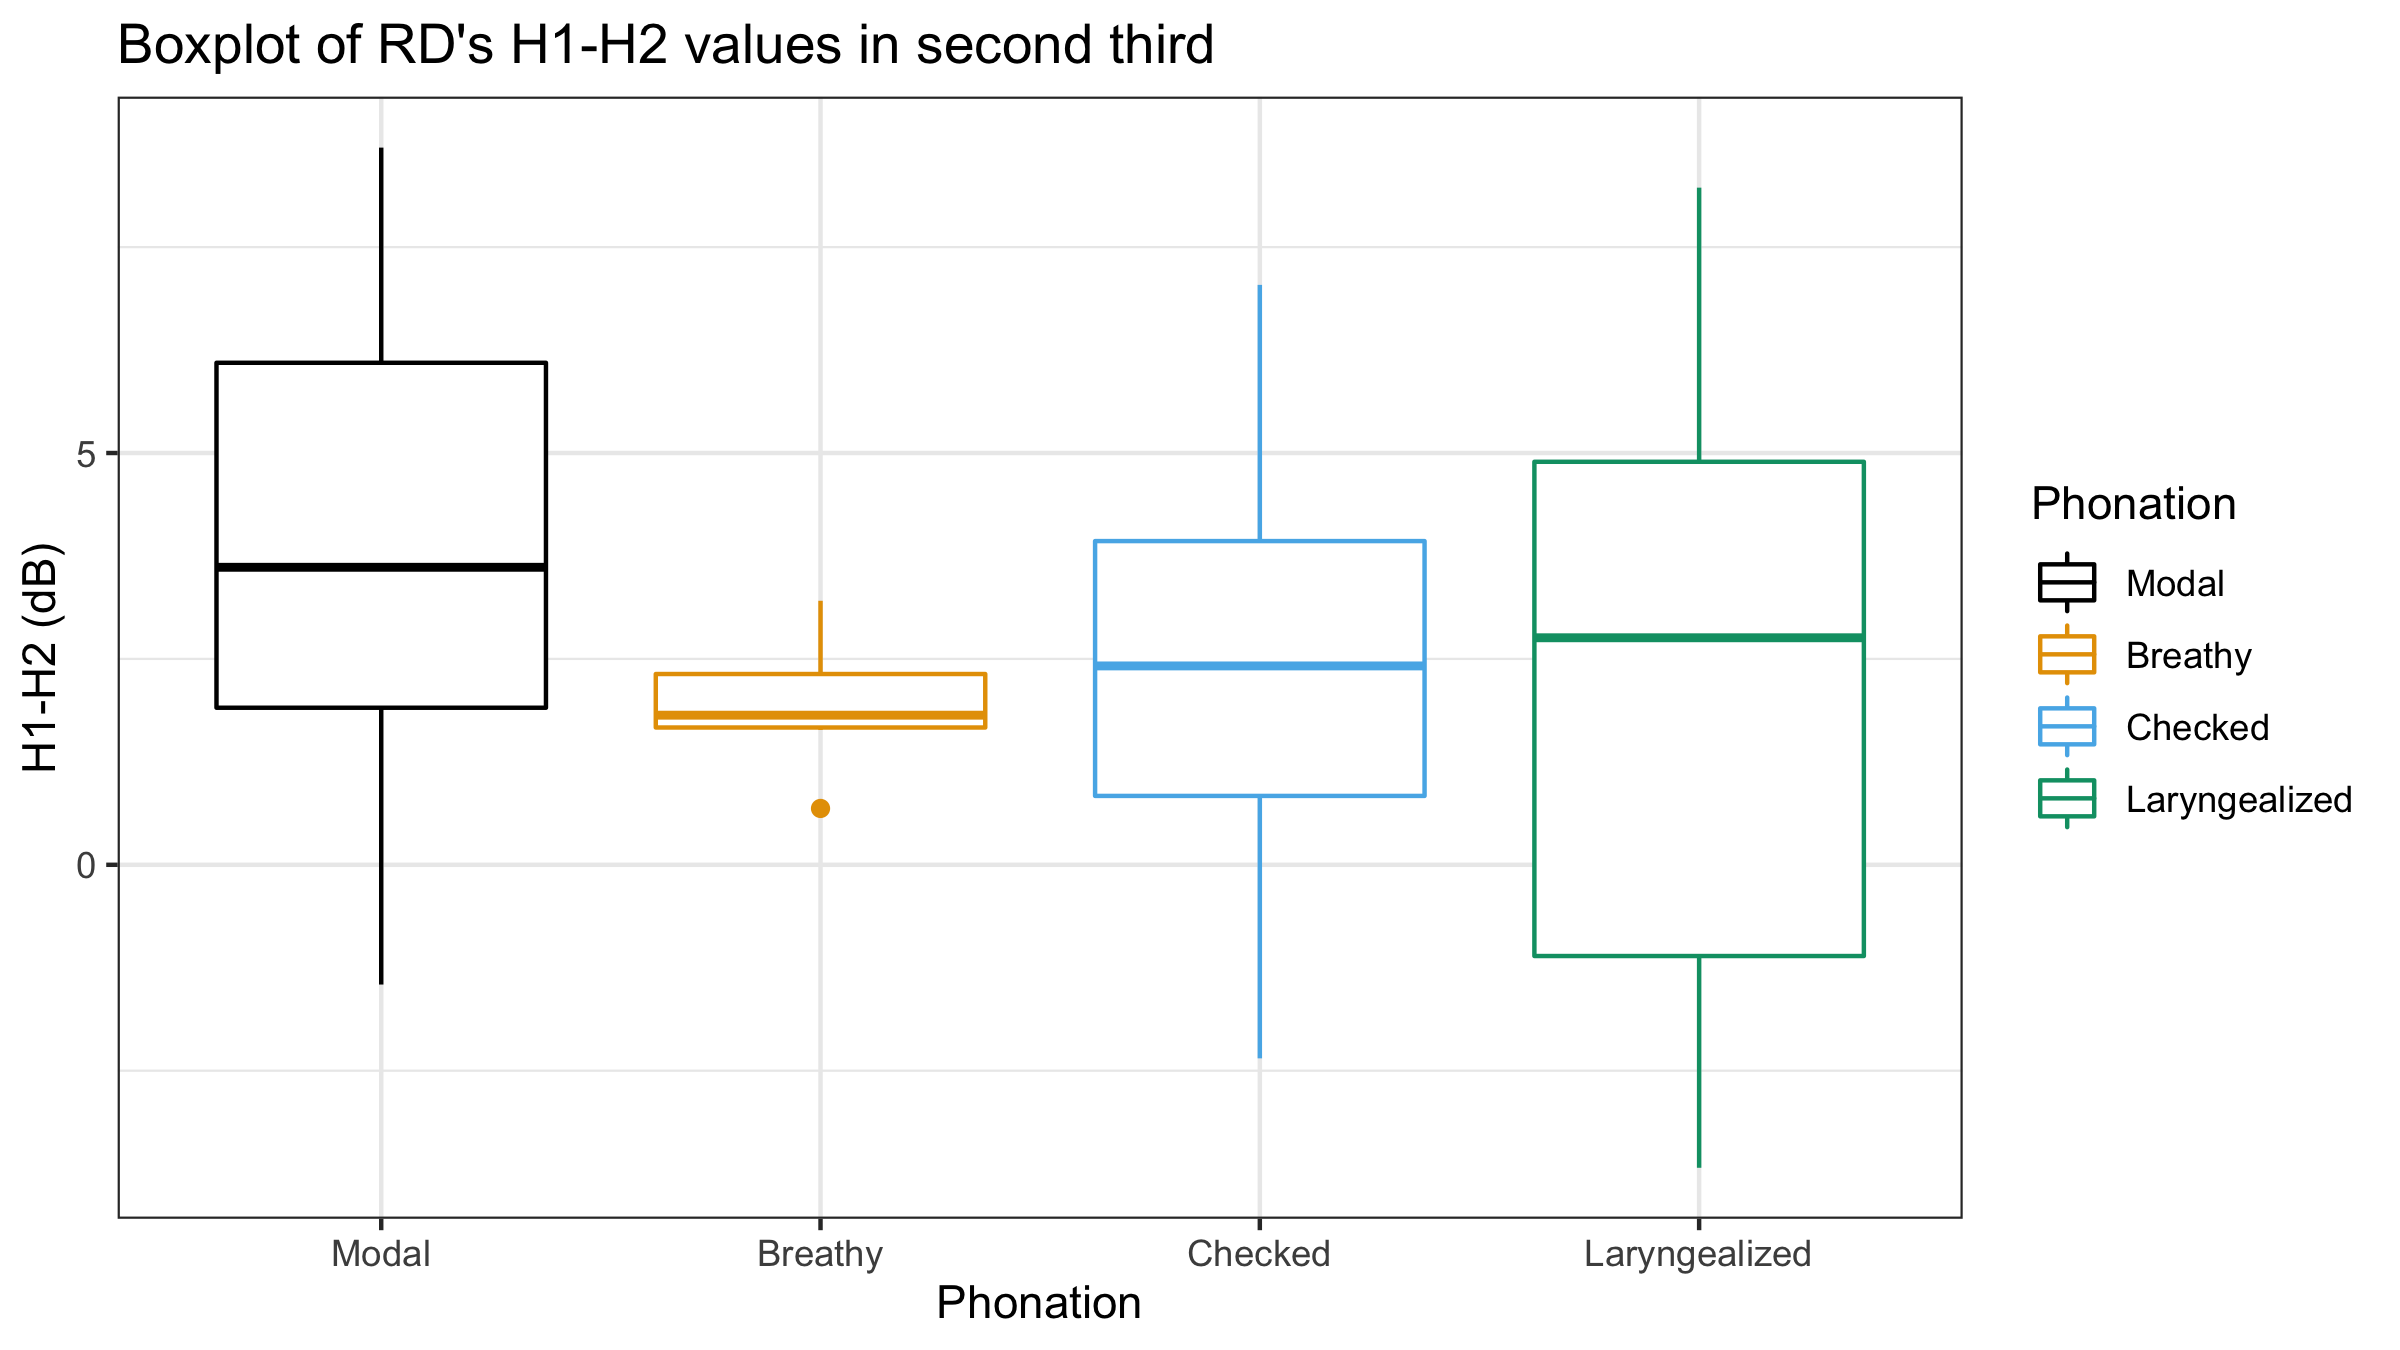
\includegraphics[width=0.9\textwidth]{Images/mean_RD_h1h2_2nd.png}
		\caption{RD's H1-H2 values.}
		\label{fig:RDh1h2second} 
	\end{subfigure}
	\caption{Mean H1-H2 values for the second third of the vowel according to each phonation type.}
	\label{fig:h1h2second}
\end{figure}

In looking at the second third of each vowel, we observe very similar results as that for the first third except that there is a more pronounced decline in values for breathy vowels with them being much lower than modal vowels, see Figure~\ref{fig:h1h2second}. The results for checked and laryngealized vowels are still nearly identical to those in Figure~\ref{fig:h1h2first}.

\begin{figure}[!ht]
	\centering
	\begin{subfigure}{.5\textwidth}
		\centering
		\includegraphics[width=0.9\textwidth]{Images/mean_FSR_h1h2_3rd.png}
		\caption{FSR's H1-H2 values.}
		\label{fig:FSRh1h2third} 
	\end{subfigure}%
	\begin{subfigure}{.5\textwidth}
		\centering
		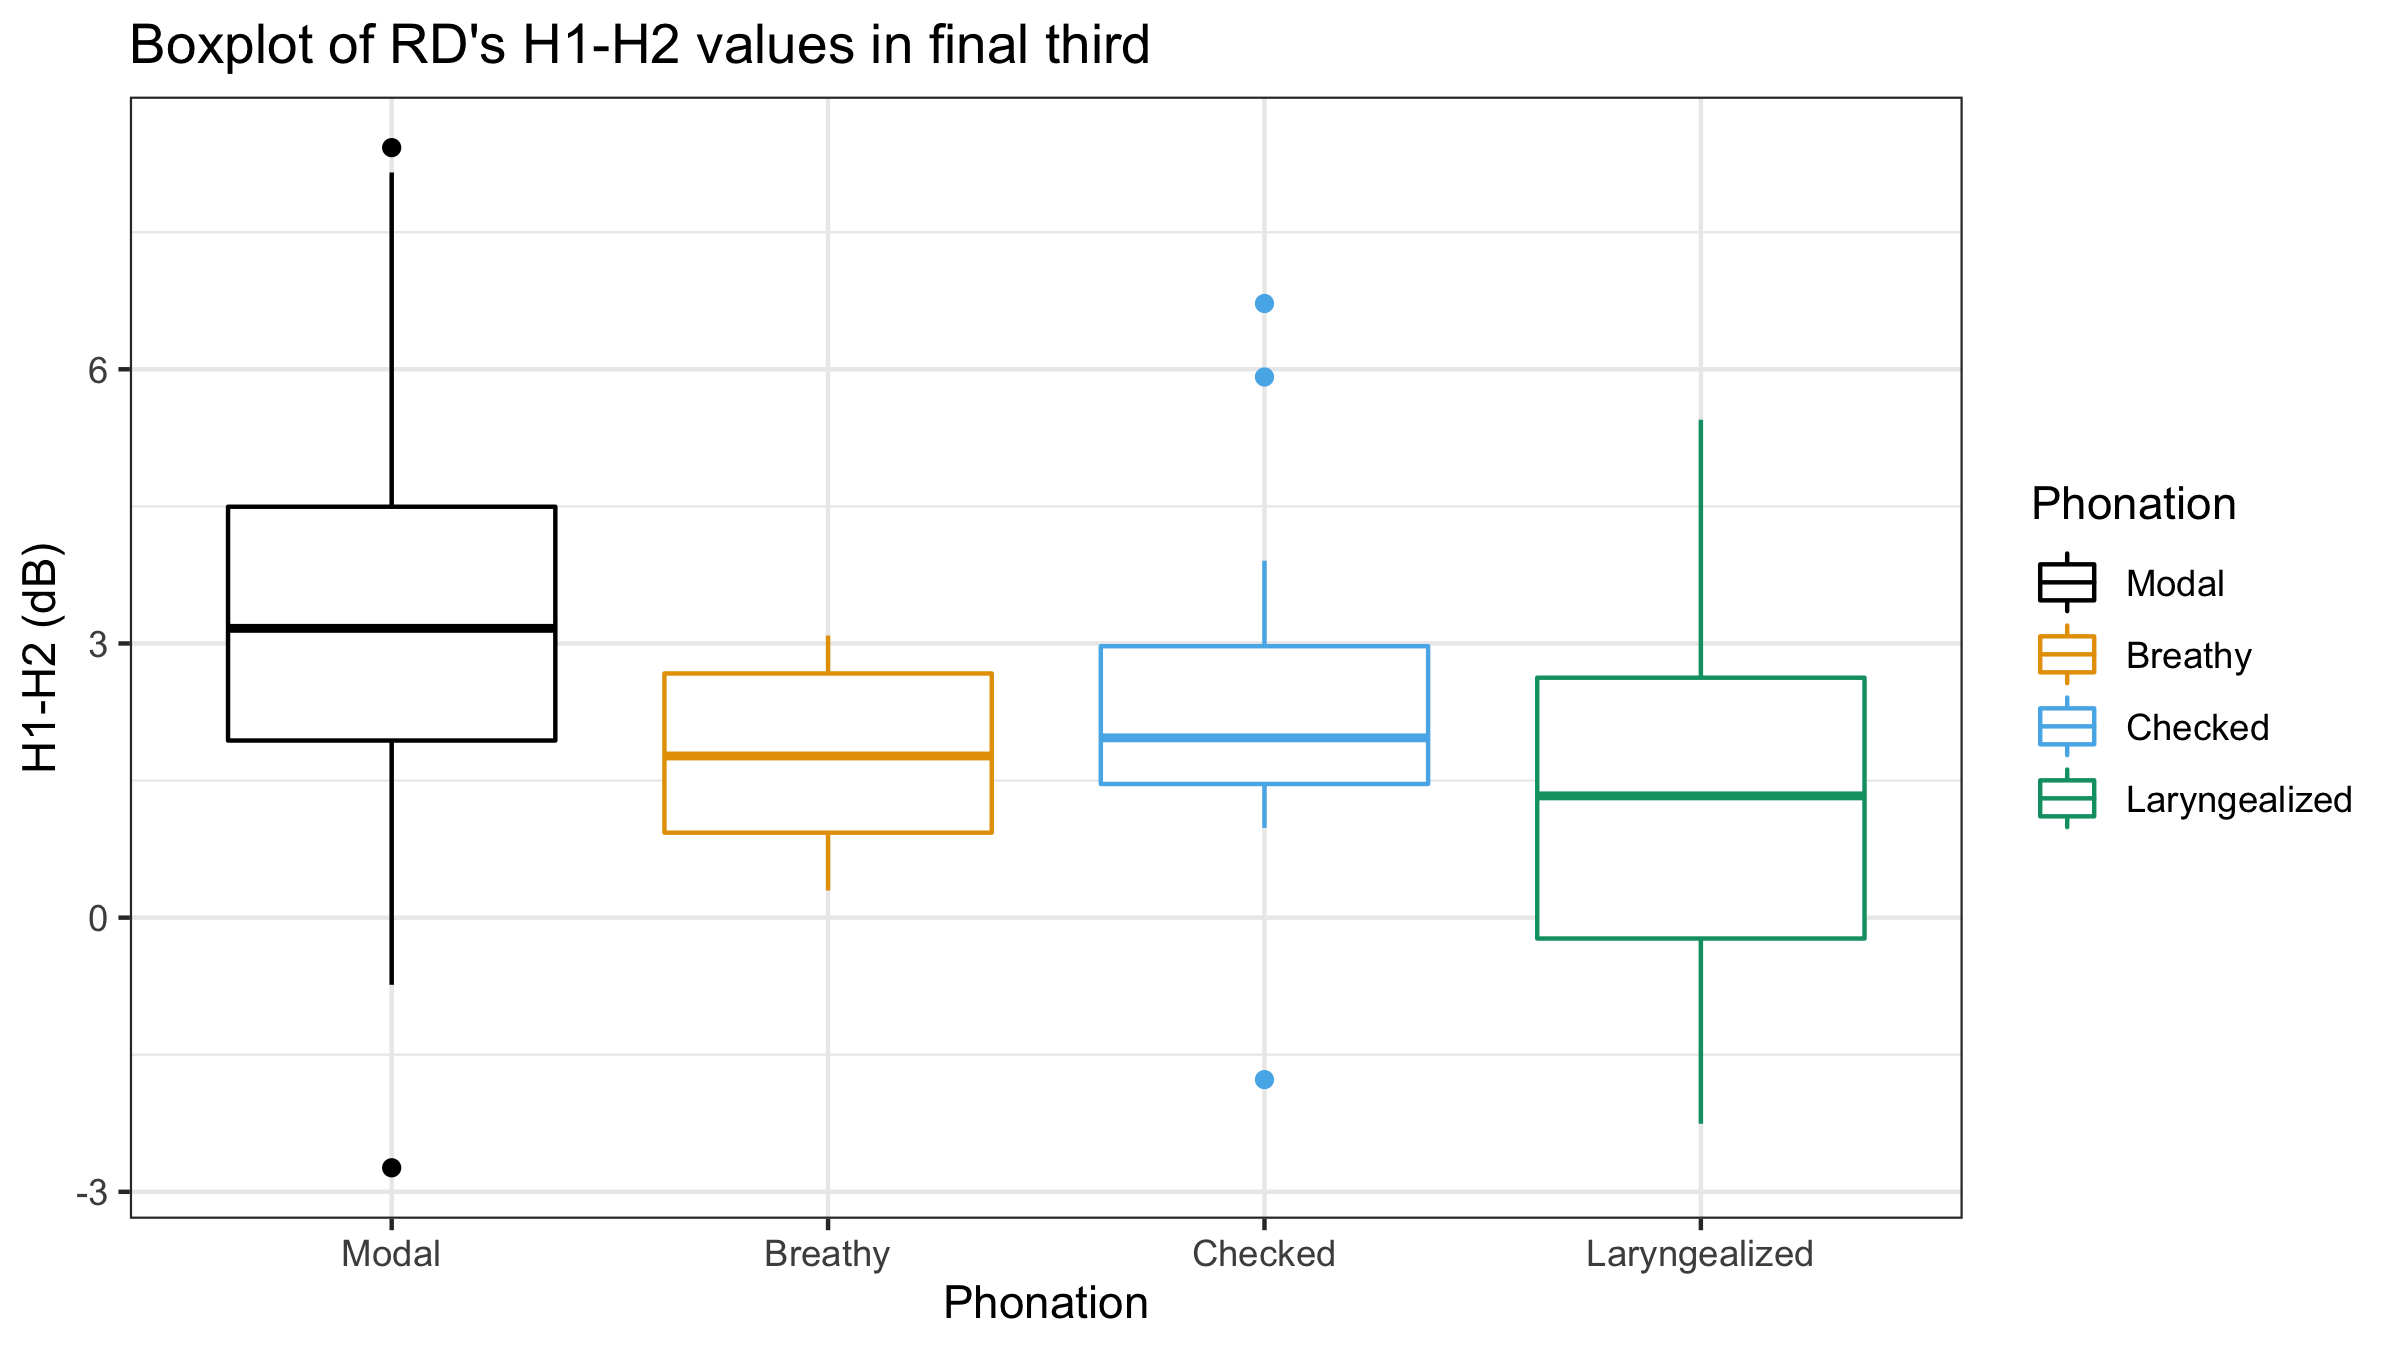
\includegraphics[width=0.9\textwidth]{Images/mean_RD_h1h2_3rd.png}
		\caption{RD's H1-H2 values.}
		\label{fig:RDh1h2third} 
	\end{subfigure}
	\caption{Mean H1-H2 values for the final third of the vowel according to each phonation type. }
	\label{fig:h1h2third}
\end{figure}

In the final third of the vowel, we continue to see breathy vowels having a lower H1-H2 value than modal vowels, which runs against our expectations for breathy vowels. Breathy vowels should have a higher value for H1-H2 than modal vowels. In FSR's values for checked and laryngealized vowels, the values are still roughly the same as those for previous portions of the vowel. RD, however, shows H1-H2 values for checked and laryngealized vowels that are lower than the values for the modal vowel. 

%------------------------------------
\subsection{H1-A3 results} \label{sec:H1A3}
%------------------------------------

Several observations quickly become apparent in turning to the H1-A3 spectral-tilt measurement that \citet{espositoVariationContrastivePhonation2010} found useful for Central Valley Zapotec. The most striking is the higher H1-A3 value found for breathy vowels in all portions of the vowel. This observation is true for both FSR and RD. 

\begin{figure}[!h]
	\centering
	\begin{subfigure}{.5\textwidth}
		\centering
		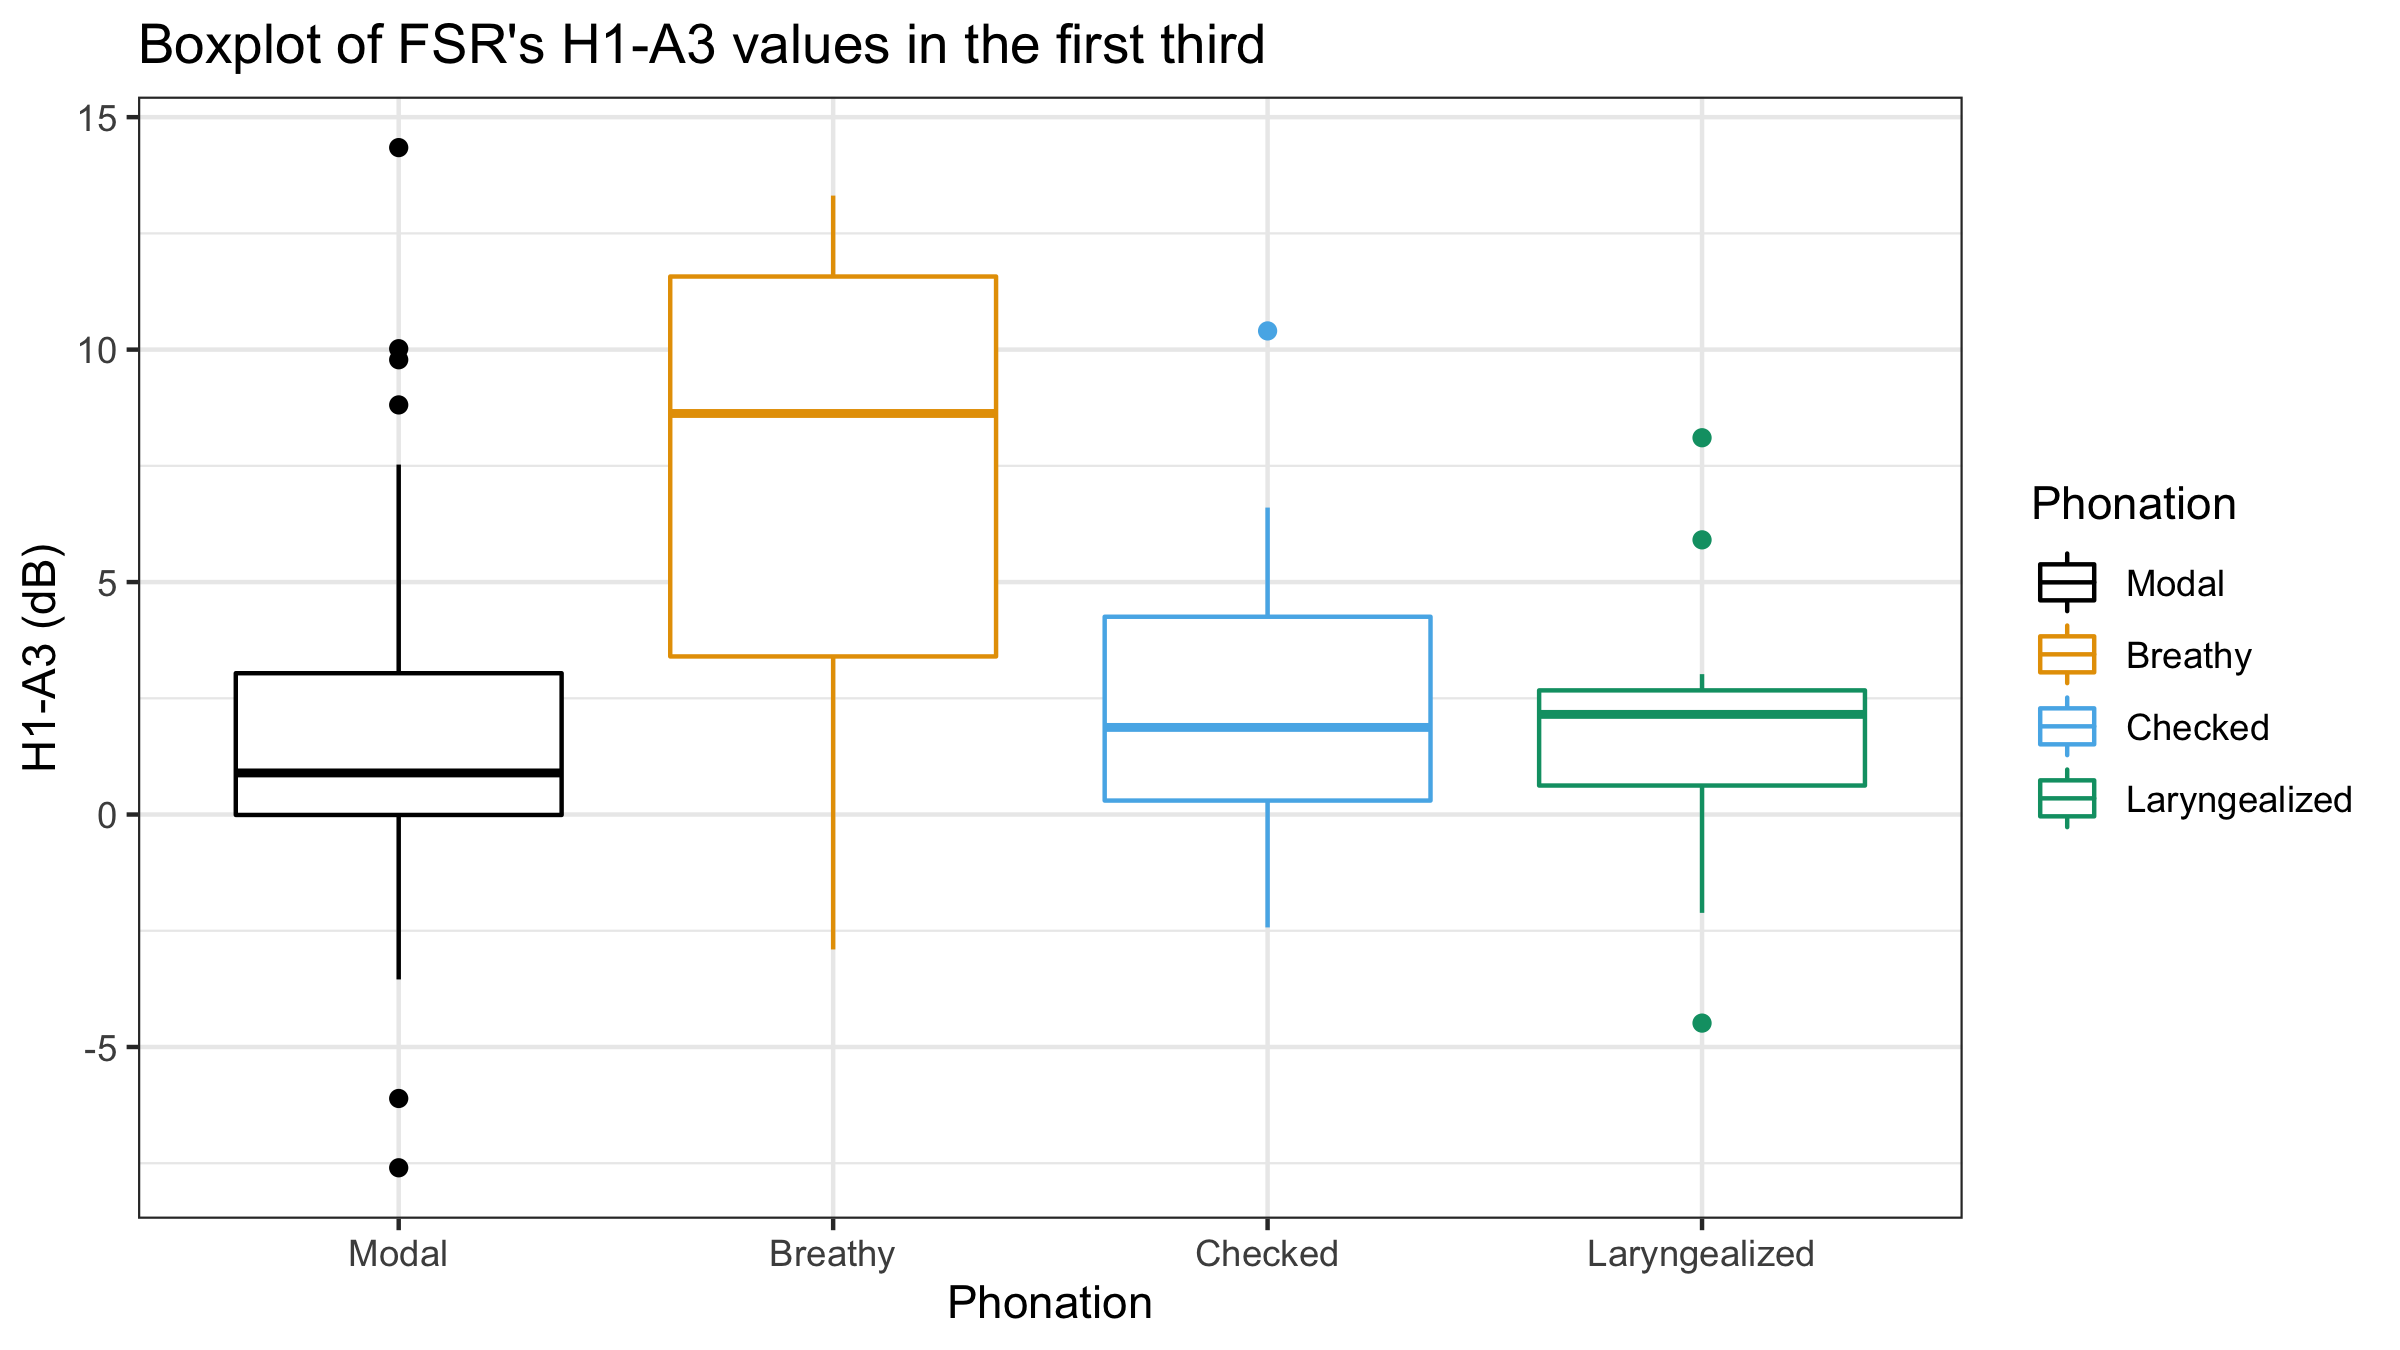
\includegraphics[width=0.9\textwidth]{Images/mean_FSR_h1a3_First.png}
		\caption{FSR's H1-A3 values.}
		\label{fig:FSRh1a3first} 
	\end{subfigure}%
	\begin{subfigure}{.5\textwidth}
		\centering
		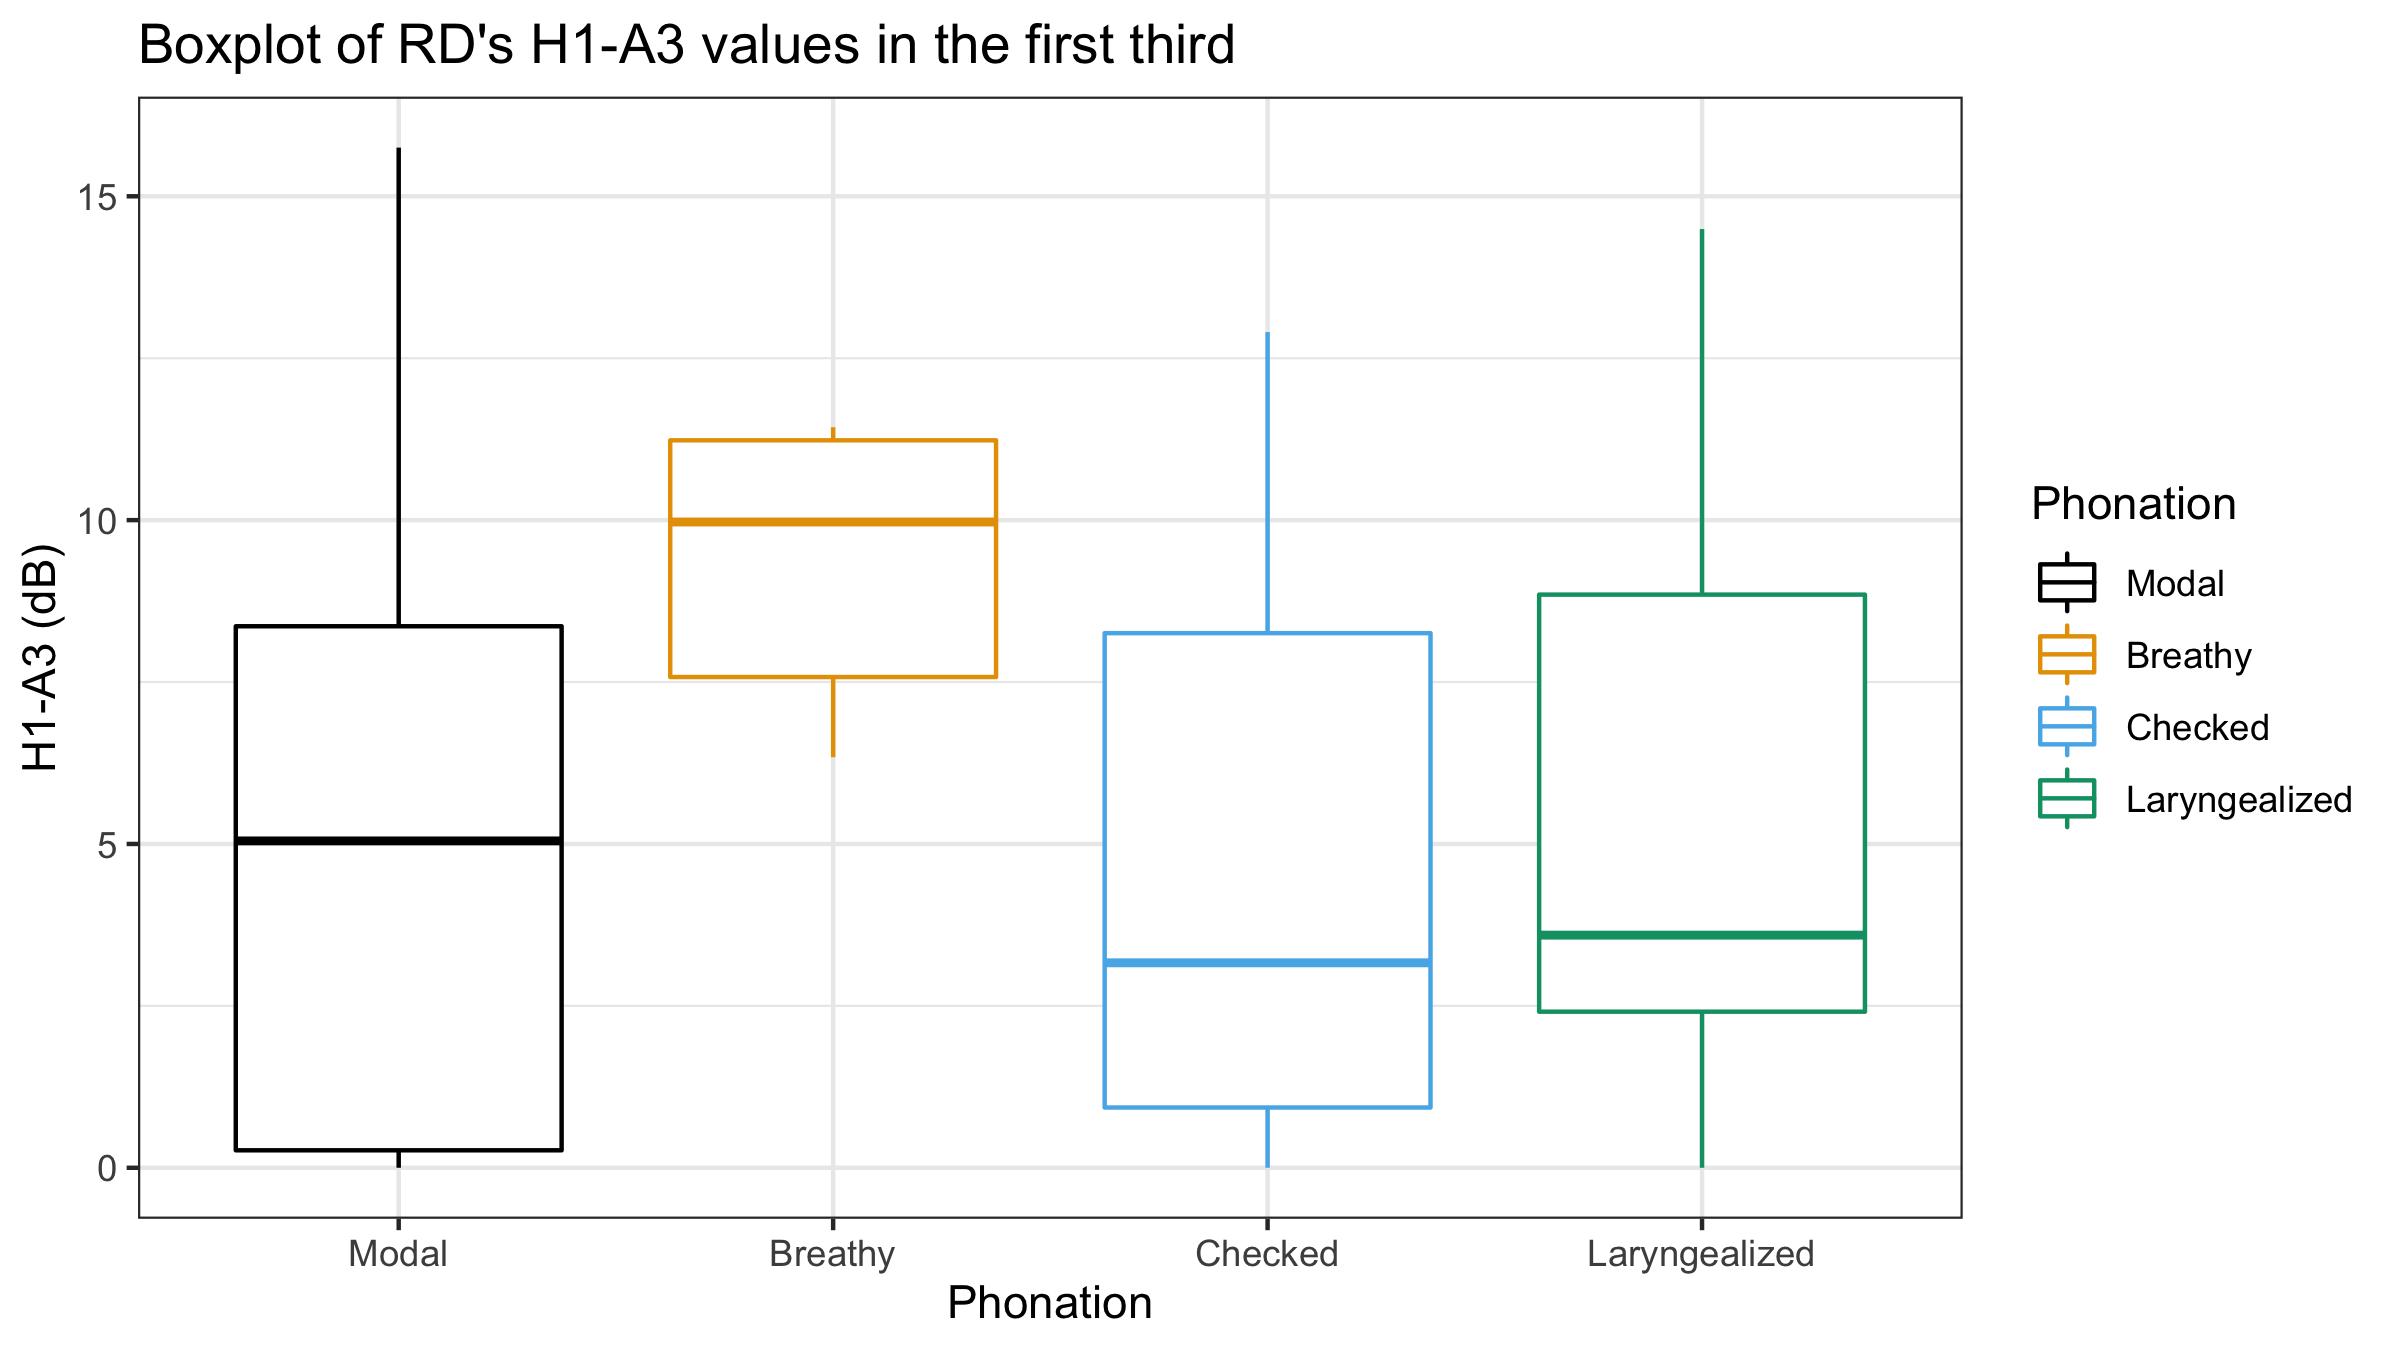
\includegraphics[width=0.9\textwidth]{Images/mean_RD_h1a3_First.png}
		\caption{RD's H1-A3 values.}
		\label{fig:RDh1a3first} 
	\end{subfigure}
	\caption{H1-A3 values for FSR (a) and RD (b) for the first third of the vowel. }
	\label{fig:h1a3first}
\end{figure}

In the first third of the vowel, RD's mean value for H1-A3 is lower than the modal's H1-A3 value. However, there is a large degree of overlap between modal, checked, and laryngealized H1-A3 values, as evidenced by the boxes covering the same regions, see Figure~\ref{fig:h1a3first}. 

\begin{figure}[!h]
	\centering
	\begin{subfigure}{.5\textwidth}
		\centering
		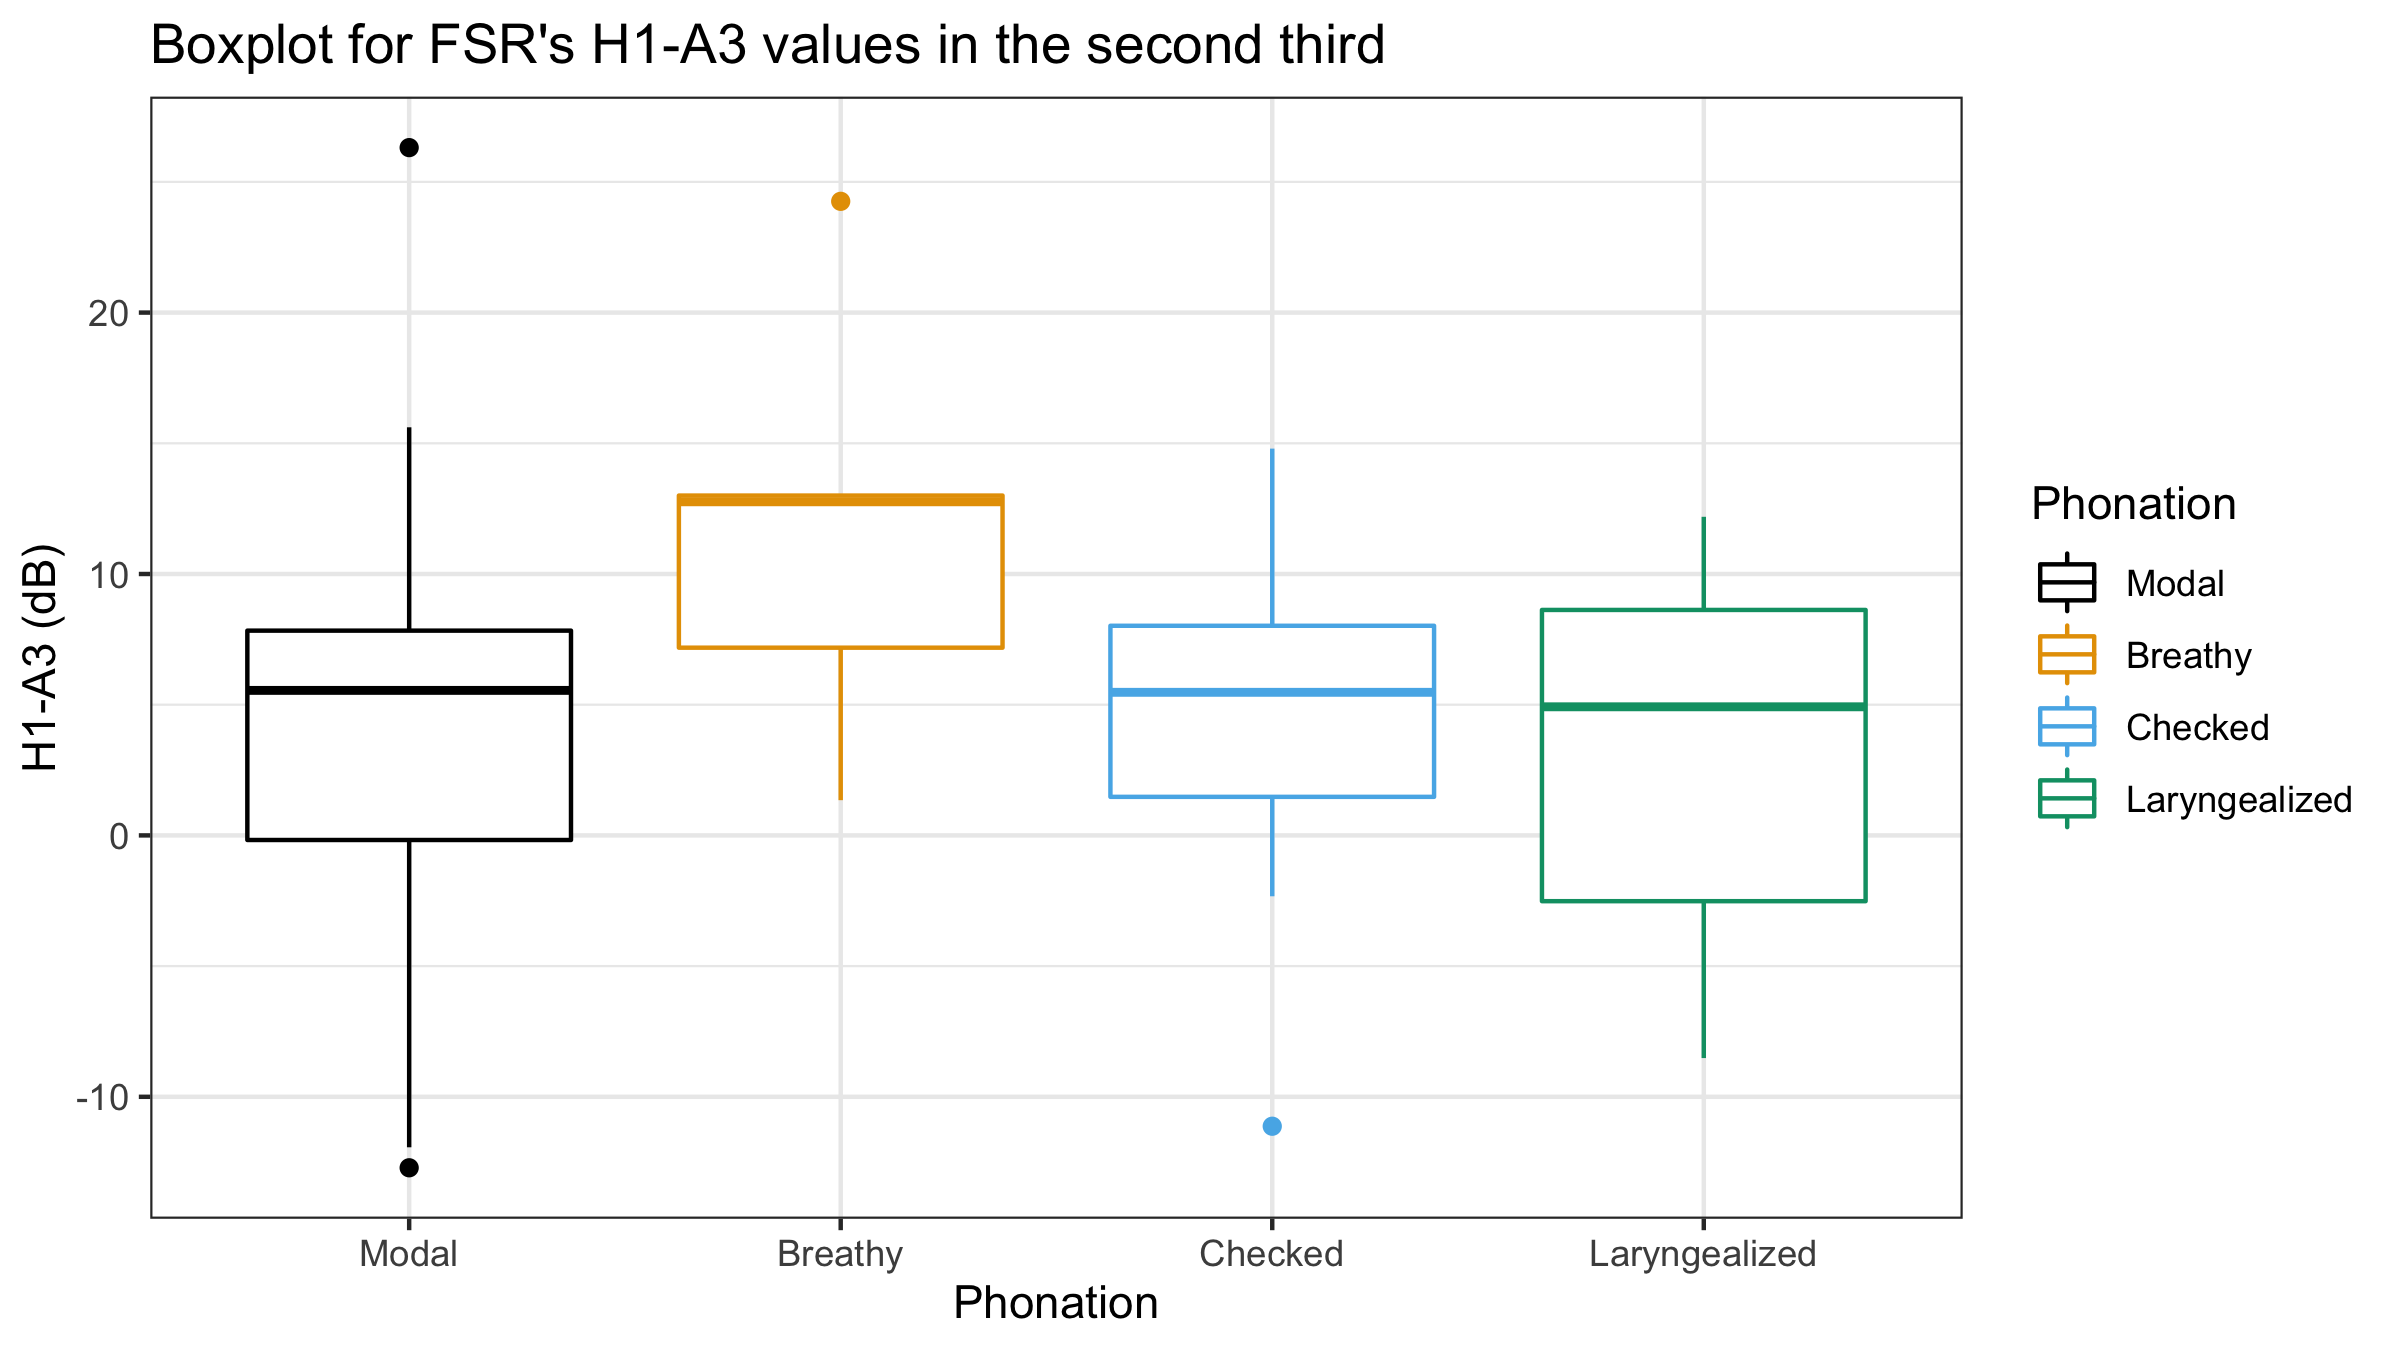
\includegraphics[width=0.9\textwidth]{Images/mean_FSR_h1a3_Second.png}
		\caption{FSR's H1-A3 values.}
		\label{fig:FSRh1a3second} 
	\end{subfigure}%
	\begin{subfigure}{.5\textwidth}
		\centering
		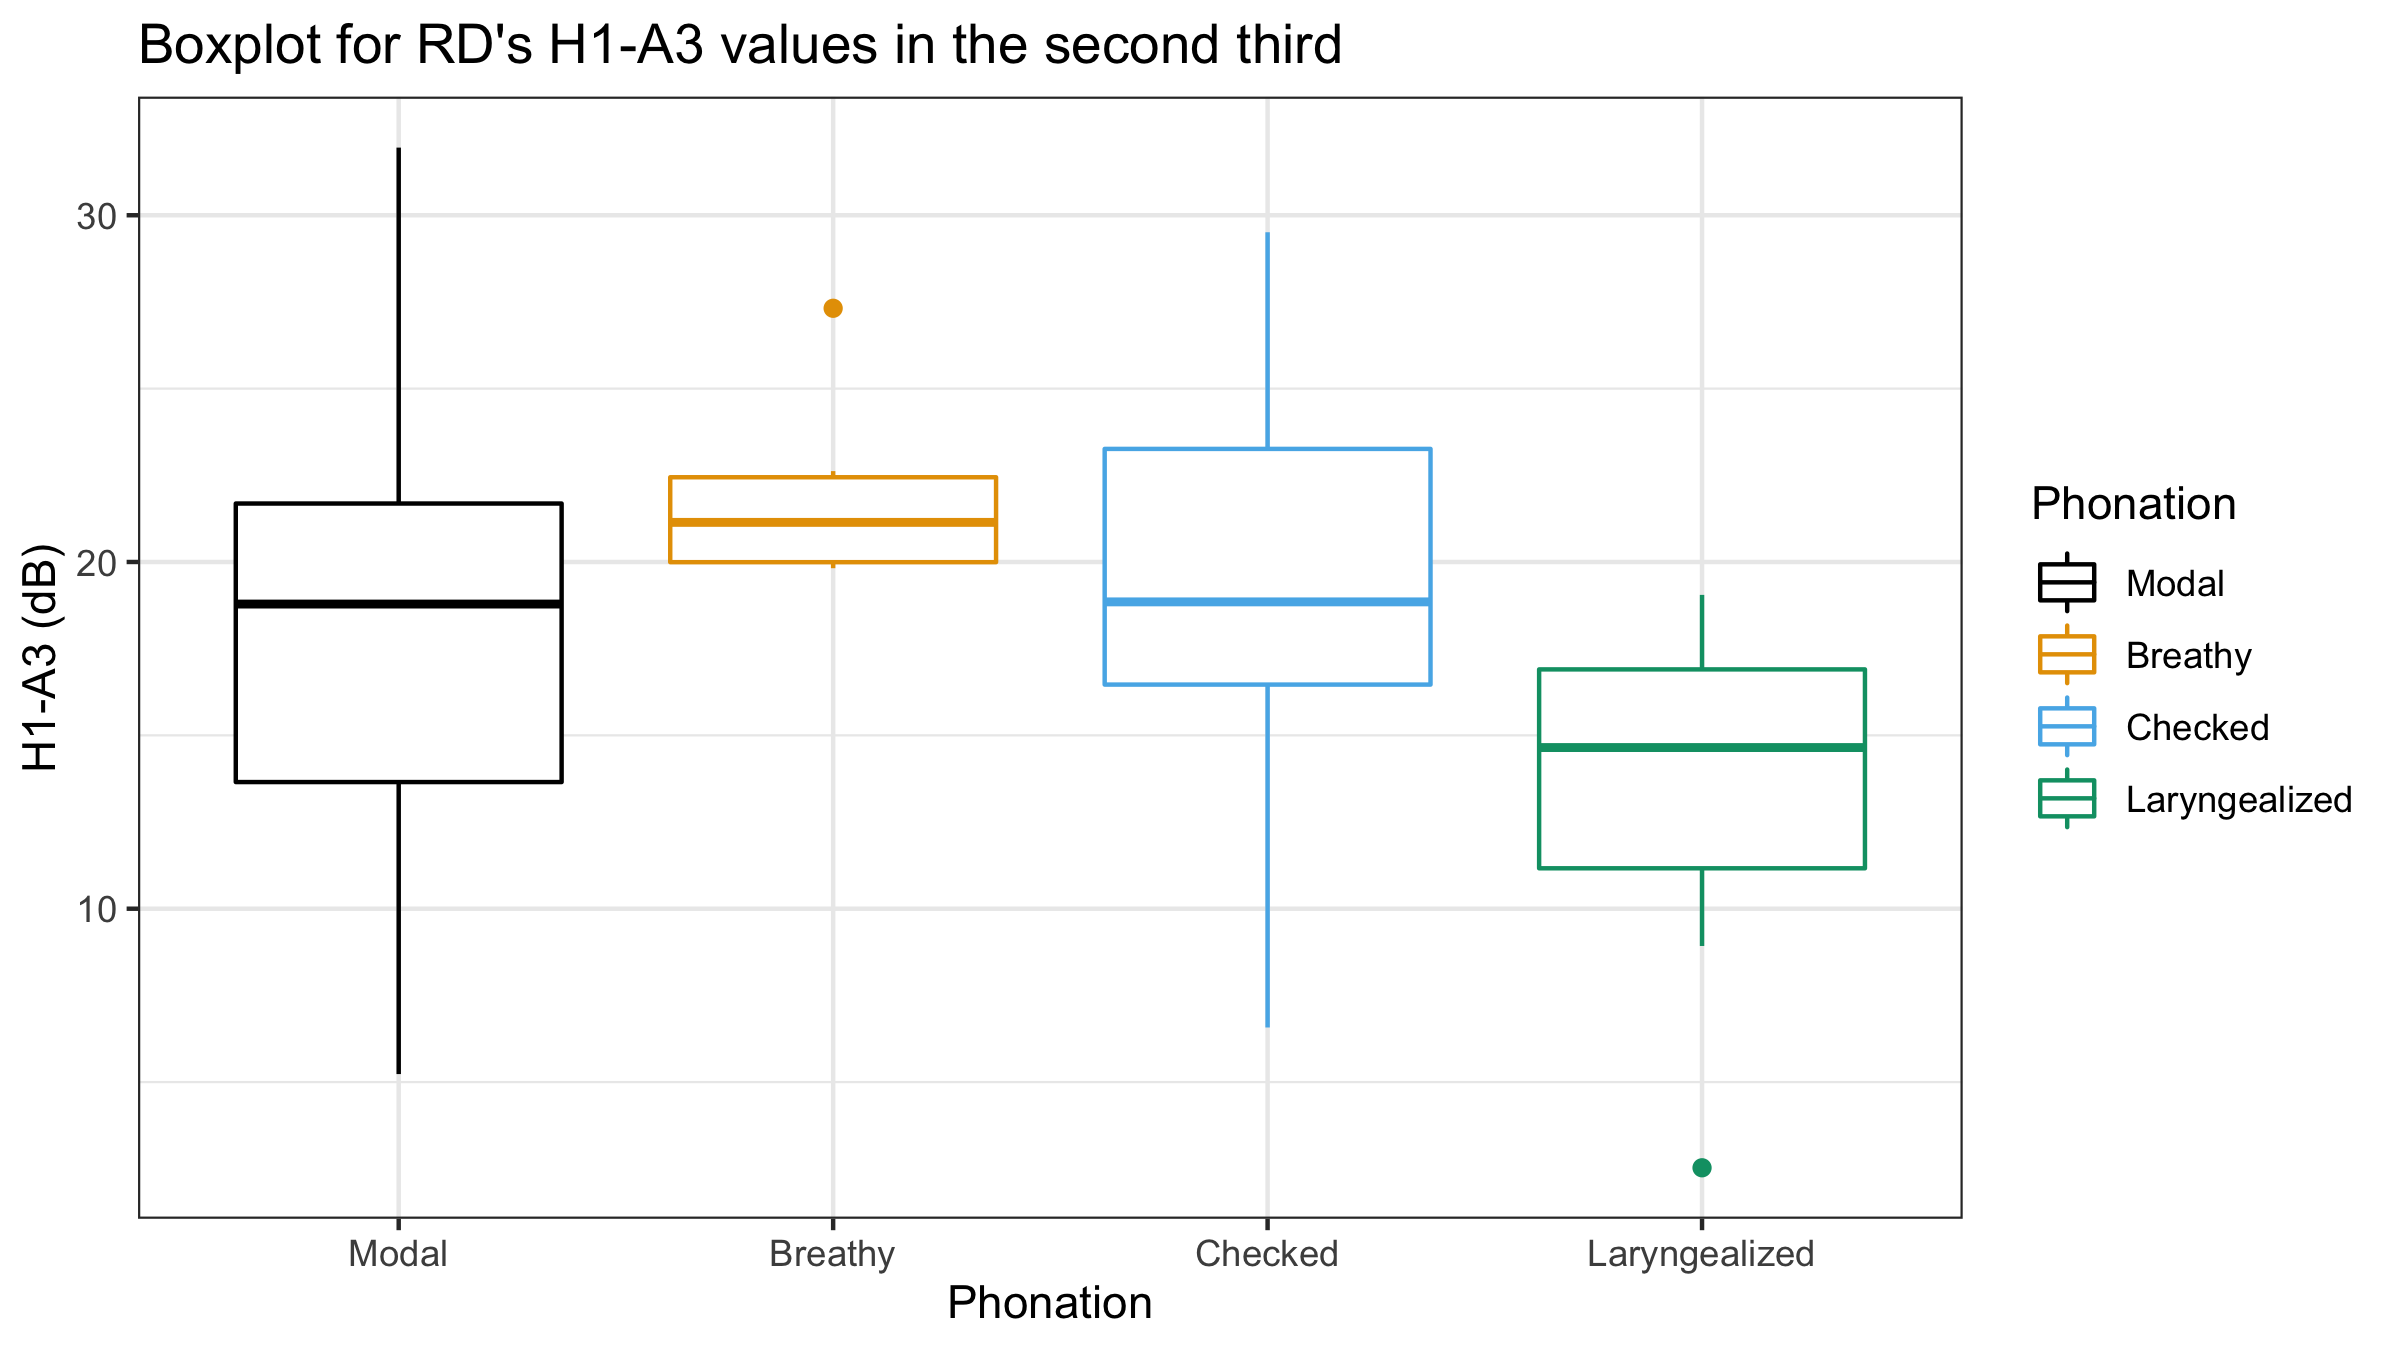
\includegraphics[width=0.9\textwidth]{Images/mean_RD_h1a3_Second.png}
		\caption{RD's H1-A3' values.}
		\label{fig:RDh1a3second} 
	\end{subfigure}
	\caption{H1-A3 values for FSR (a) and RD (b) for the second third of the vowel. }
	\label{fig:h1a3second}
\end{figure}

In the second third of the vowel, Figure~\ref{fig:h1a3second}, the breathy vowel continues to be higher than the modal vowel. The checked and laryngealized vowels H1-A3 values for FSR are uninformative because of the large degree of overlap. For RD, these same measurements show a lower H1-A3 value than the modal's, which is consistent with creakier productions of vowels. This lower H1-A3 continues throughout the rest of the vowel for laryngealized vowels; see Figure~\ref{fig:RDh1a3third}. This behavior is consistent with the observation that RD performs creaky voice throughout their production of laryngealized vowels. For the checked vowels, the measurements are very similar to those of the modal vowel. 

In looking at the final portion of the vowels, Figure~\ref{fig:h1a3third}, the measurements continue to show similar behavior to the second portion for both FSR and RD. However, one exception is the lower H1-A3 value for FSR's checked vowels, suggesting that FSR produces a period of creakiness in the last portion of the vowel.

\begin{figure}[!ht]
	\centering
	\begin{subfigure}{.5\textwidth}
		\centering
		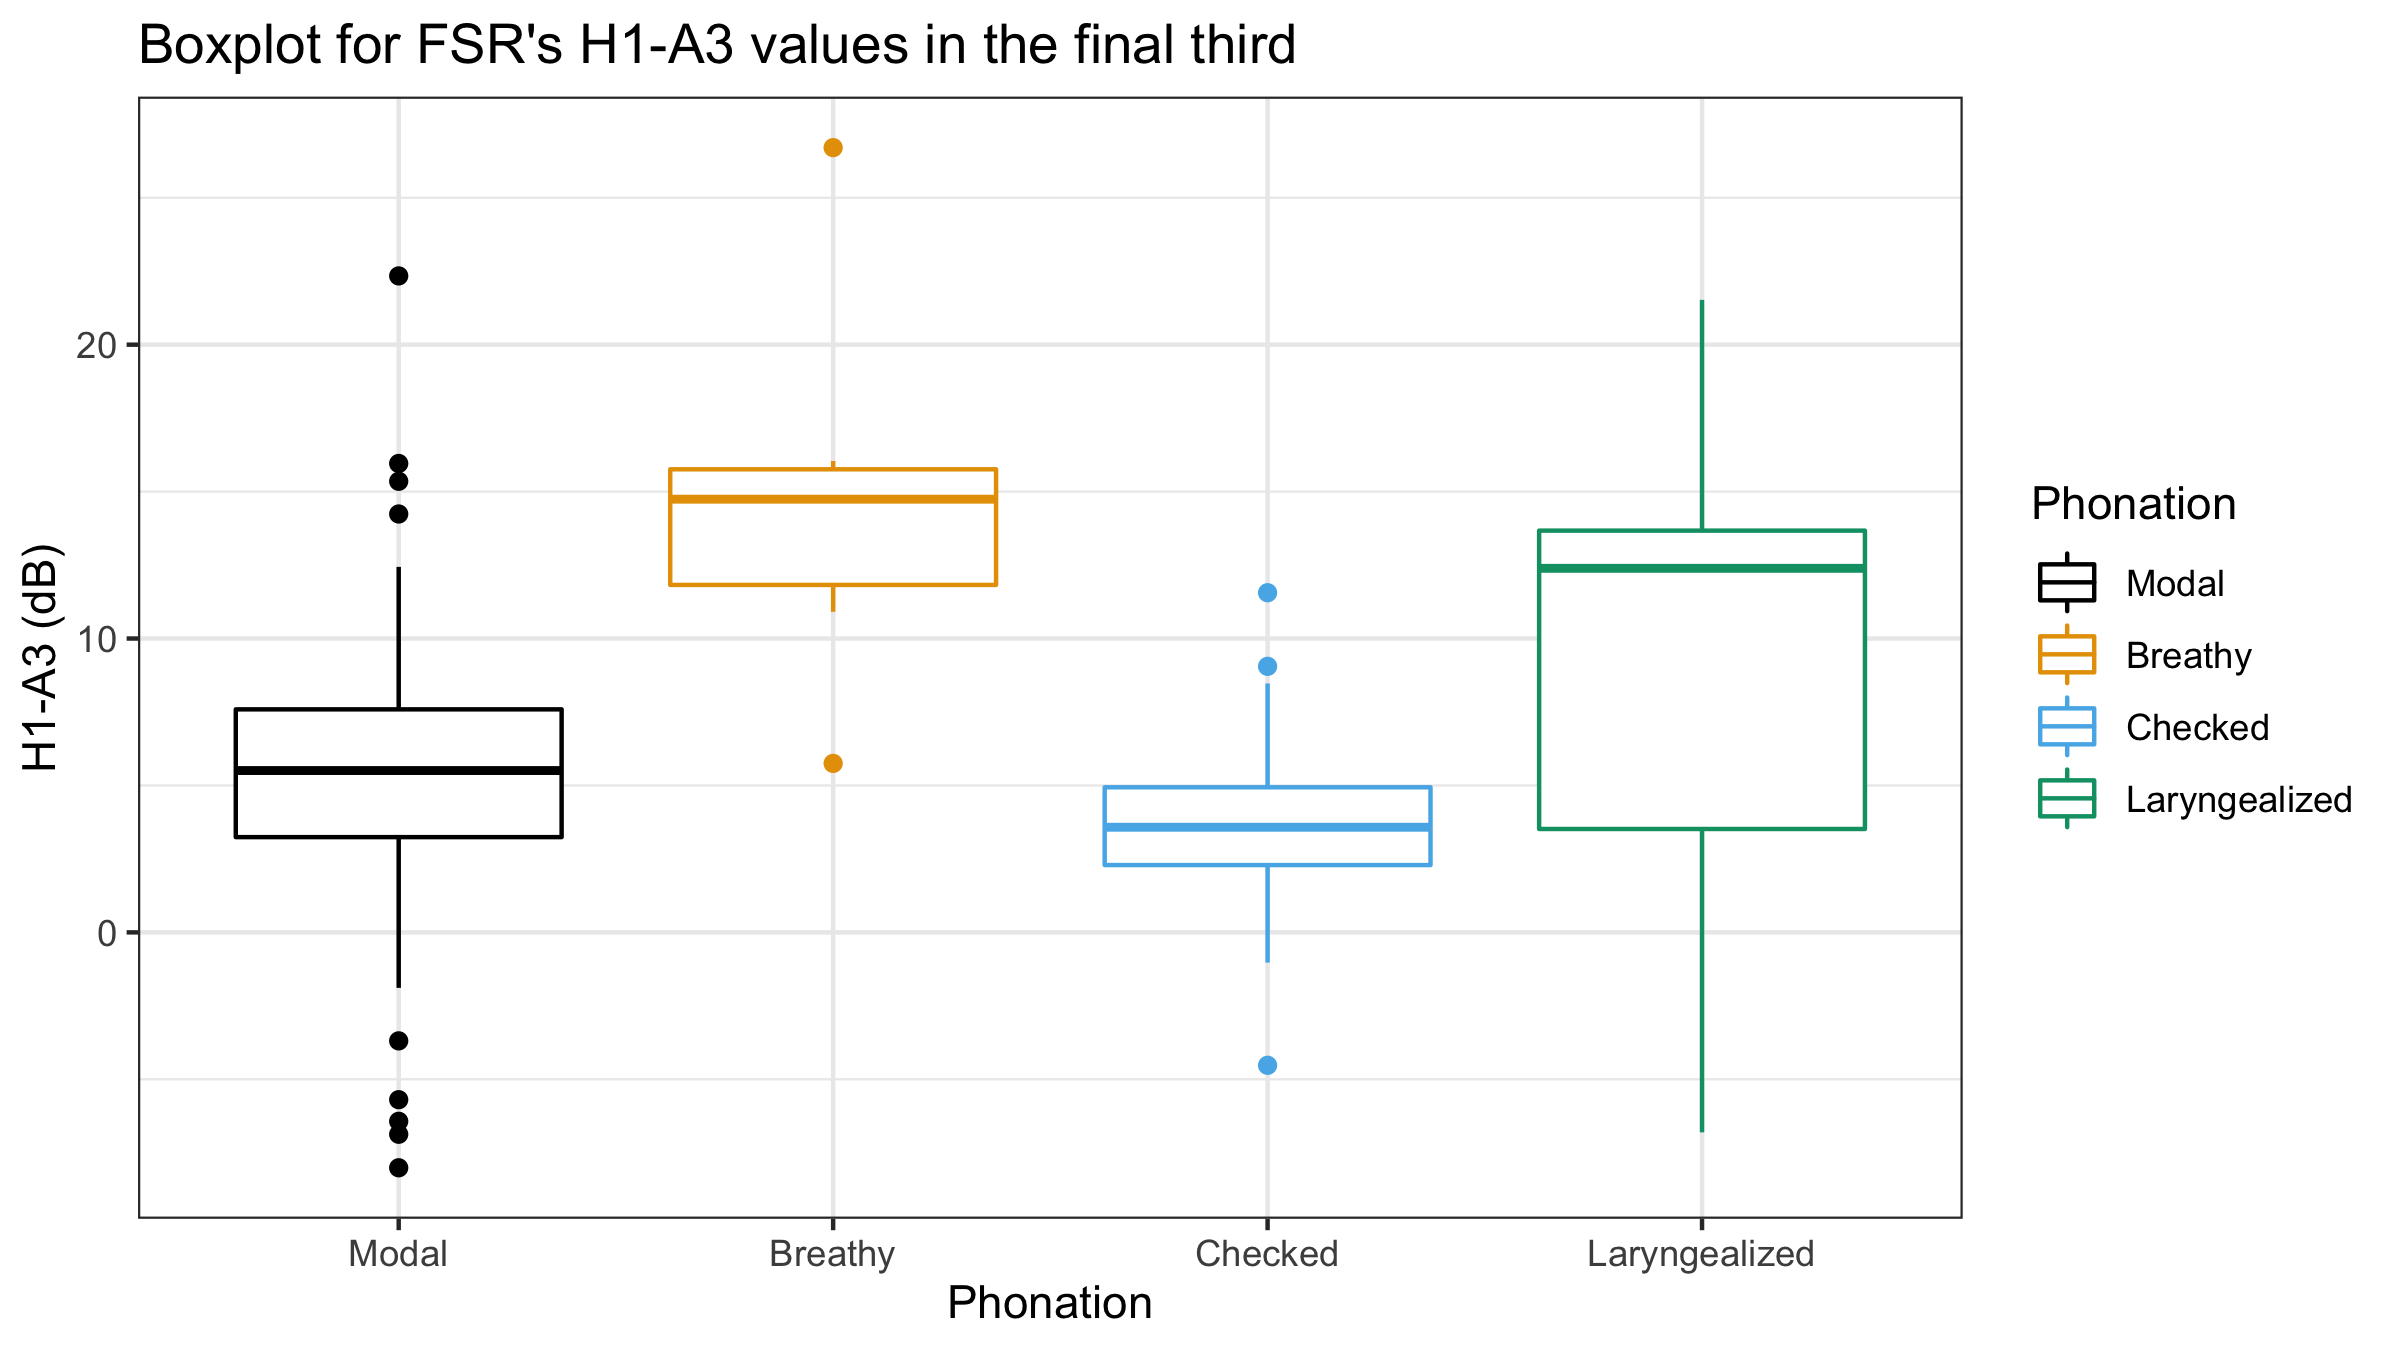
\includegraphics[width=0.9\textwidth]{Images/mean_FSR_h1a3_third.png}
		\caption{FSR's H1-A3 values.}
		\label{fig:FSRh1a3third} 
	\end{subfigure}%
	\begin{subfigure}{.5\textwidth}
		\centering
		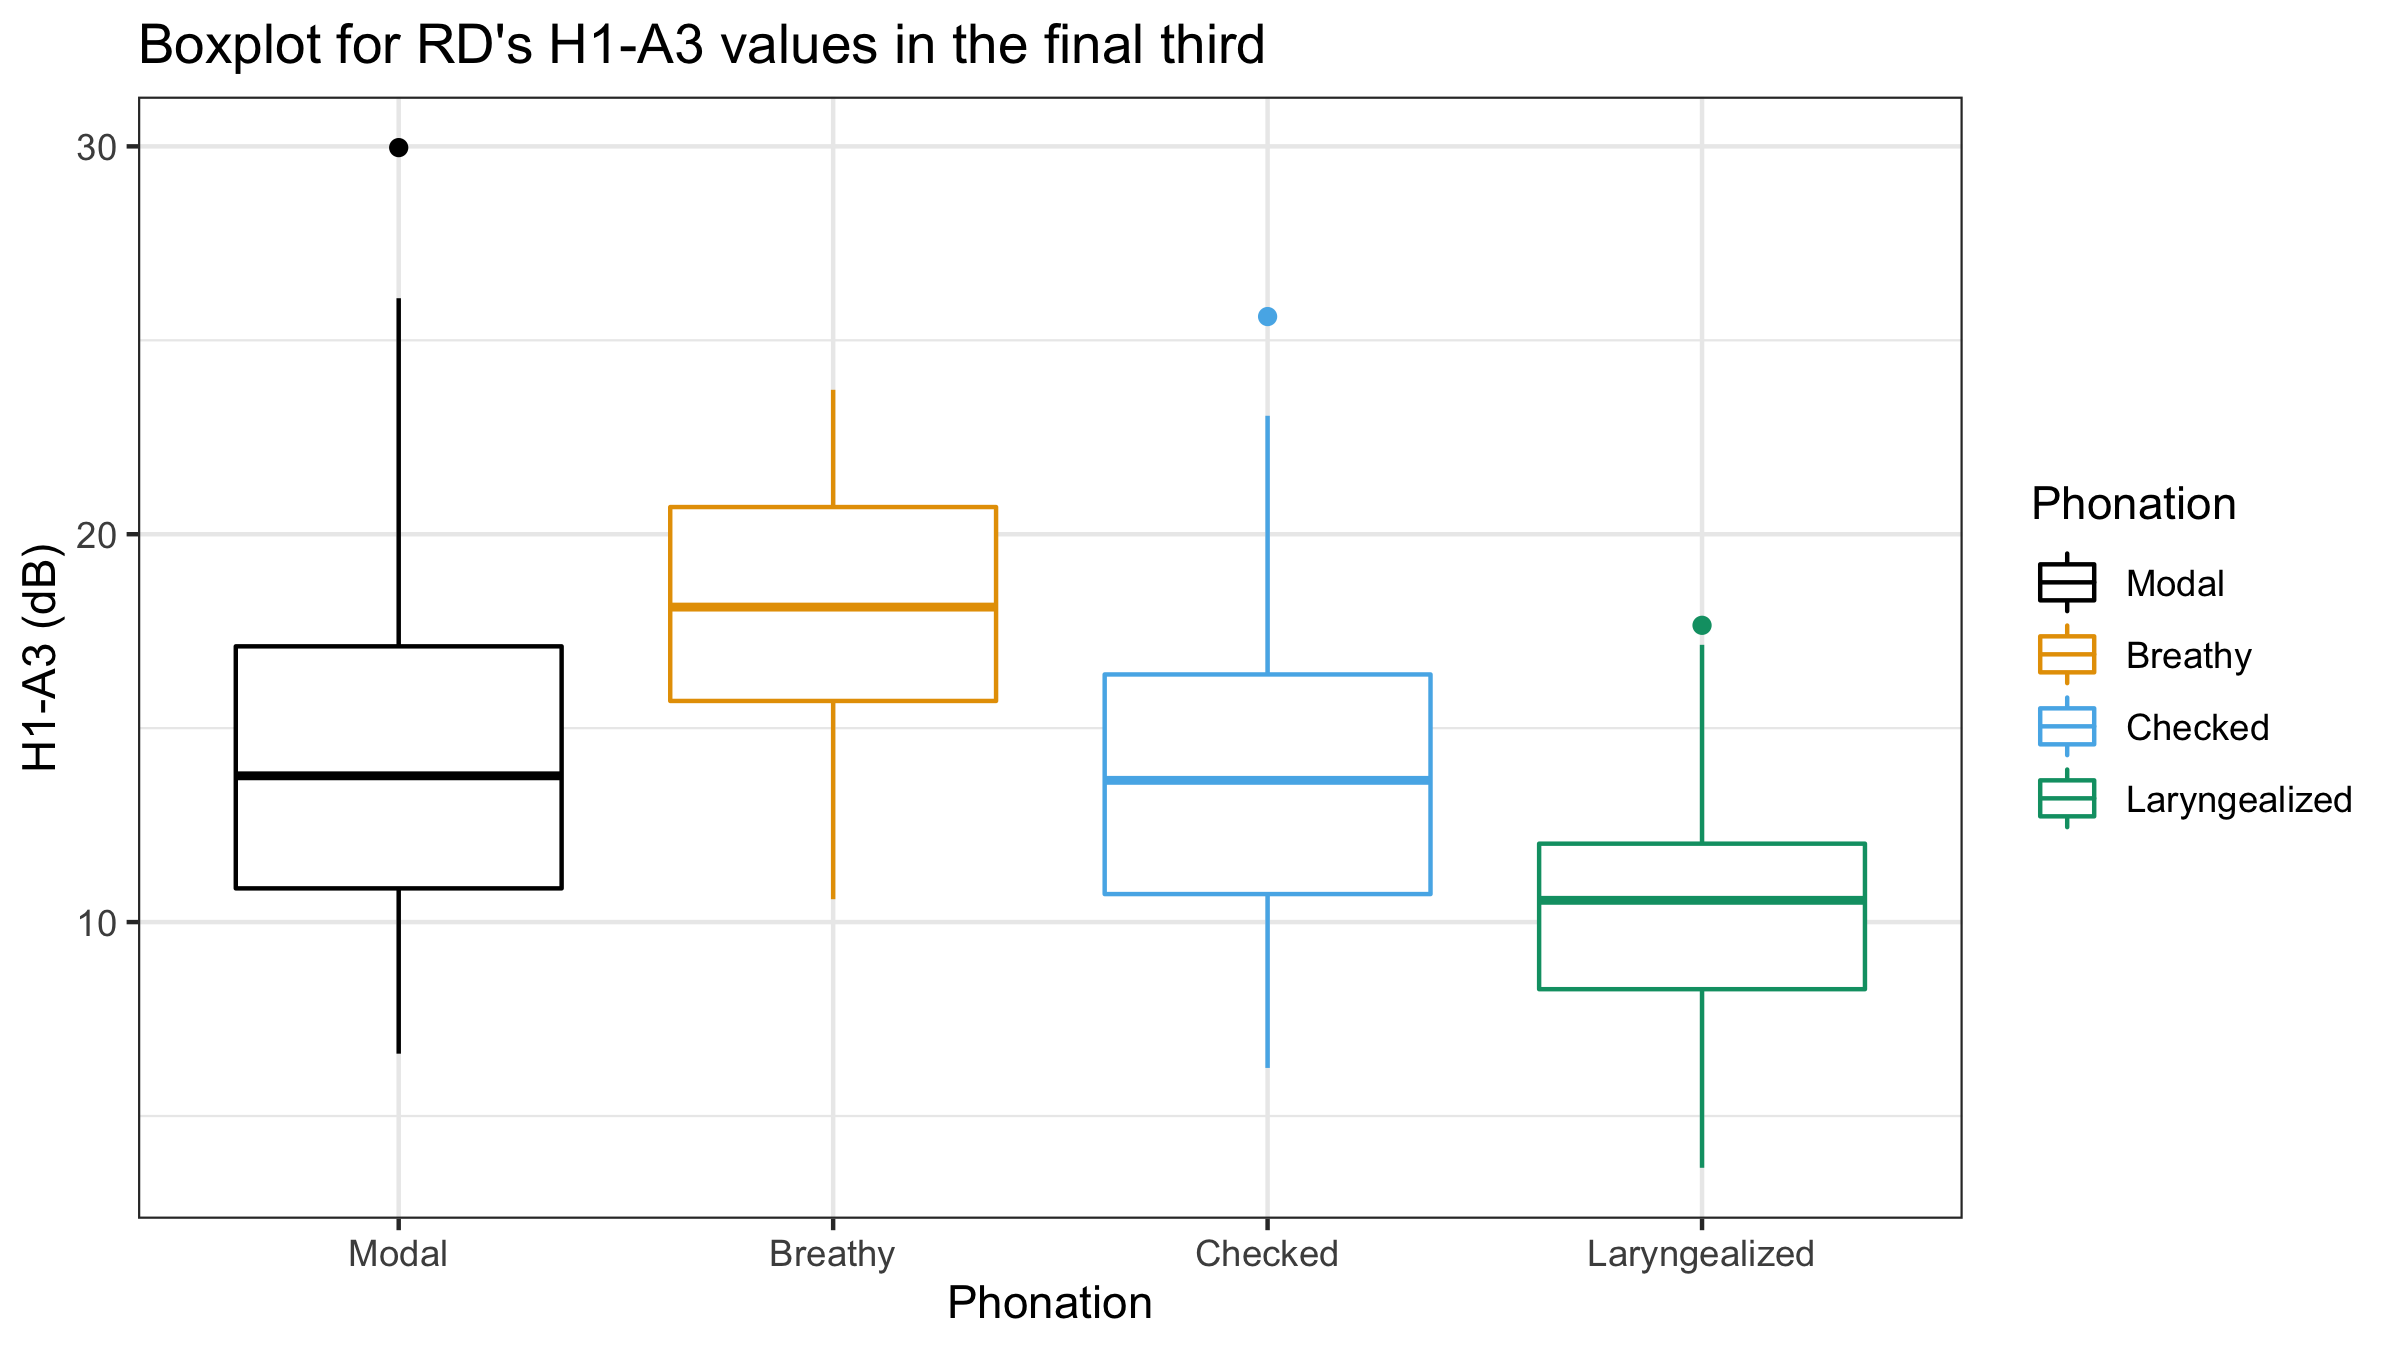
\includegraphics[width=0.9\textwidth]{Images/mean_RD_h1a3_third.png}
		\caption{RD's H1-A3 values.}
		\label{fig:RDh1a3third} 
	\end{subfigure}
	\caption{H1-A3 values for FSR (a) and RD (b) for the final third of the vowel. }
	\label{fig:h1a3third}
\end{figure}

%------------------------------------
\subsection{CPP results} \label{sec:CPP}
%------------------------------------

As previously mentioned at the start of Section~\ref{sec:Acoustics}, another measurement that is frequently encountered with spectral-tilt measurements is a Cepstral Peak Prominence (CPP) measurement \citep{hillenbrandAcousticCorrelatesBreathy1994}, which is a type of harmonics-to-noise ratio and indicates whether or not there is any aperiodicity in the signal. 

A CPP measurement for any vowel with non-modal phonation should be lower than the CPP measurement for modal vowels. When evaluating the CPP measurements for the same vowels and portions of a vowel, there are several observations that readily become apparent. The most noticeable observation is that for both speakers the breathy vowel's CPP value is consistently higher than the modal vowel's CPP value, which is opposite what is typically observed for non-modal phonation. When evaluating the checked vowel's CPP values, FSR had a lower value in the first third but the rest of the vowel shows values that are comparable to the modal vowel. For RD's checked vowels, the CPP shows that the mean is in fact lower than the modals in Figures~\ref{fig:RDcppfirst}, \ref{fig:RDcppsecond}, and \ref{fig:RDcppthird} but there is a large overlap in values. 

Laryngealized vowels show a different pattern. For FSR, the laryngealized vowel's CPP value is lower than the modal's CPP value in the second-third of the vowel only. For RD, however, the laryngealized vowels have the roughly the same values as the modal vowels throughout the thirds. 

\begin{figure}[!ht]
	\centering
	\begin{subfigure}{.5\textwidth}
		\centering
		\includegraphics[width=0.9\textwidth]{Images/mean_FSR_cpp_First.png}
		\caption{FSR's CPP values.}
		\label{fig:FSRcppfirst} 
	\end{subfigure}%
	\begin{subfigure}{.5\textwidth}
		\centering
		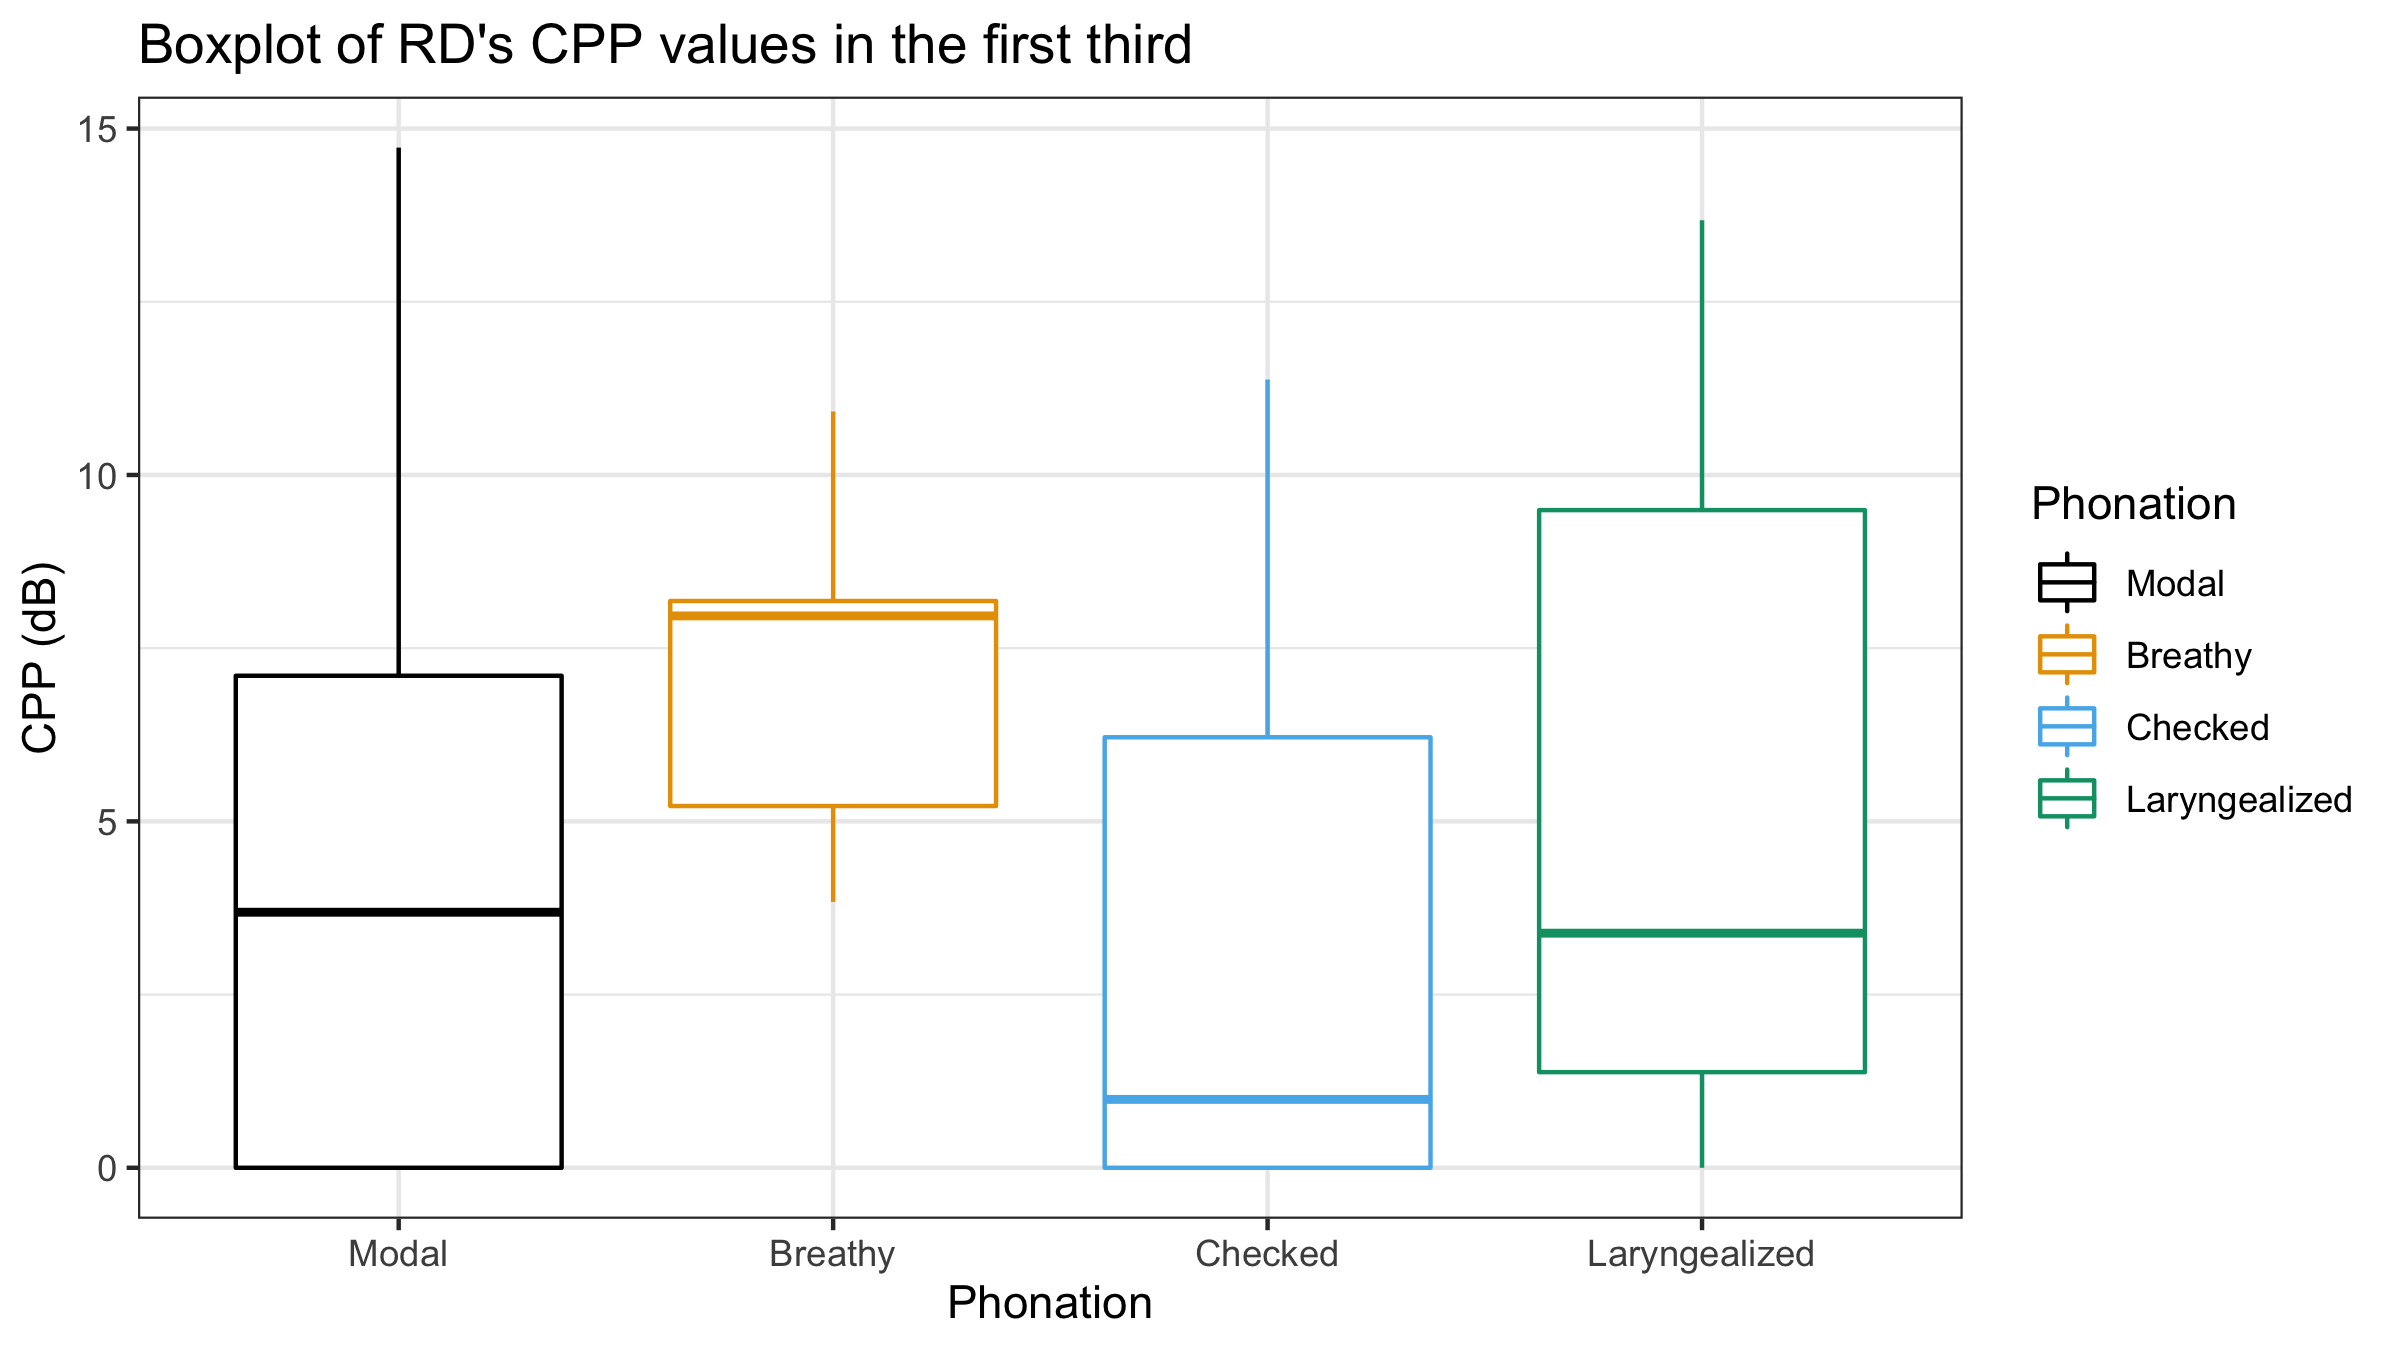
\includegraphics[width=0.9\textwidth]{Images/mean_RD_cpp_First.png}
		\caption{RD's CPP values.}
		\label{fig:RDcppfirst} 
	\end{subfigure}
	\caption{CPP values for FSR (a) and RD (b) for the first third of the vowel. }
	\label{fig:cppfirst}
\end{figure}

\begin{figure}[!ht]
	\centering
	\begin{subfigure}{.5\textwidth}
		\centering
		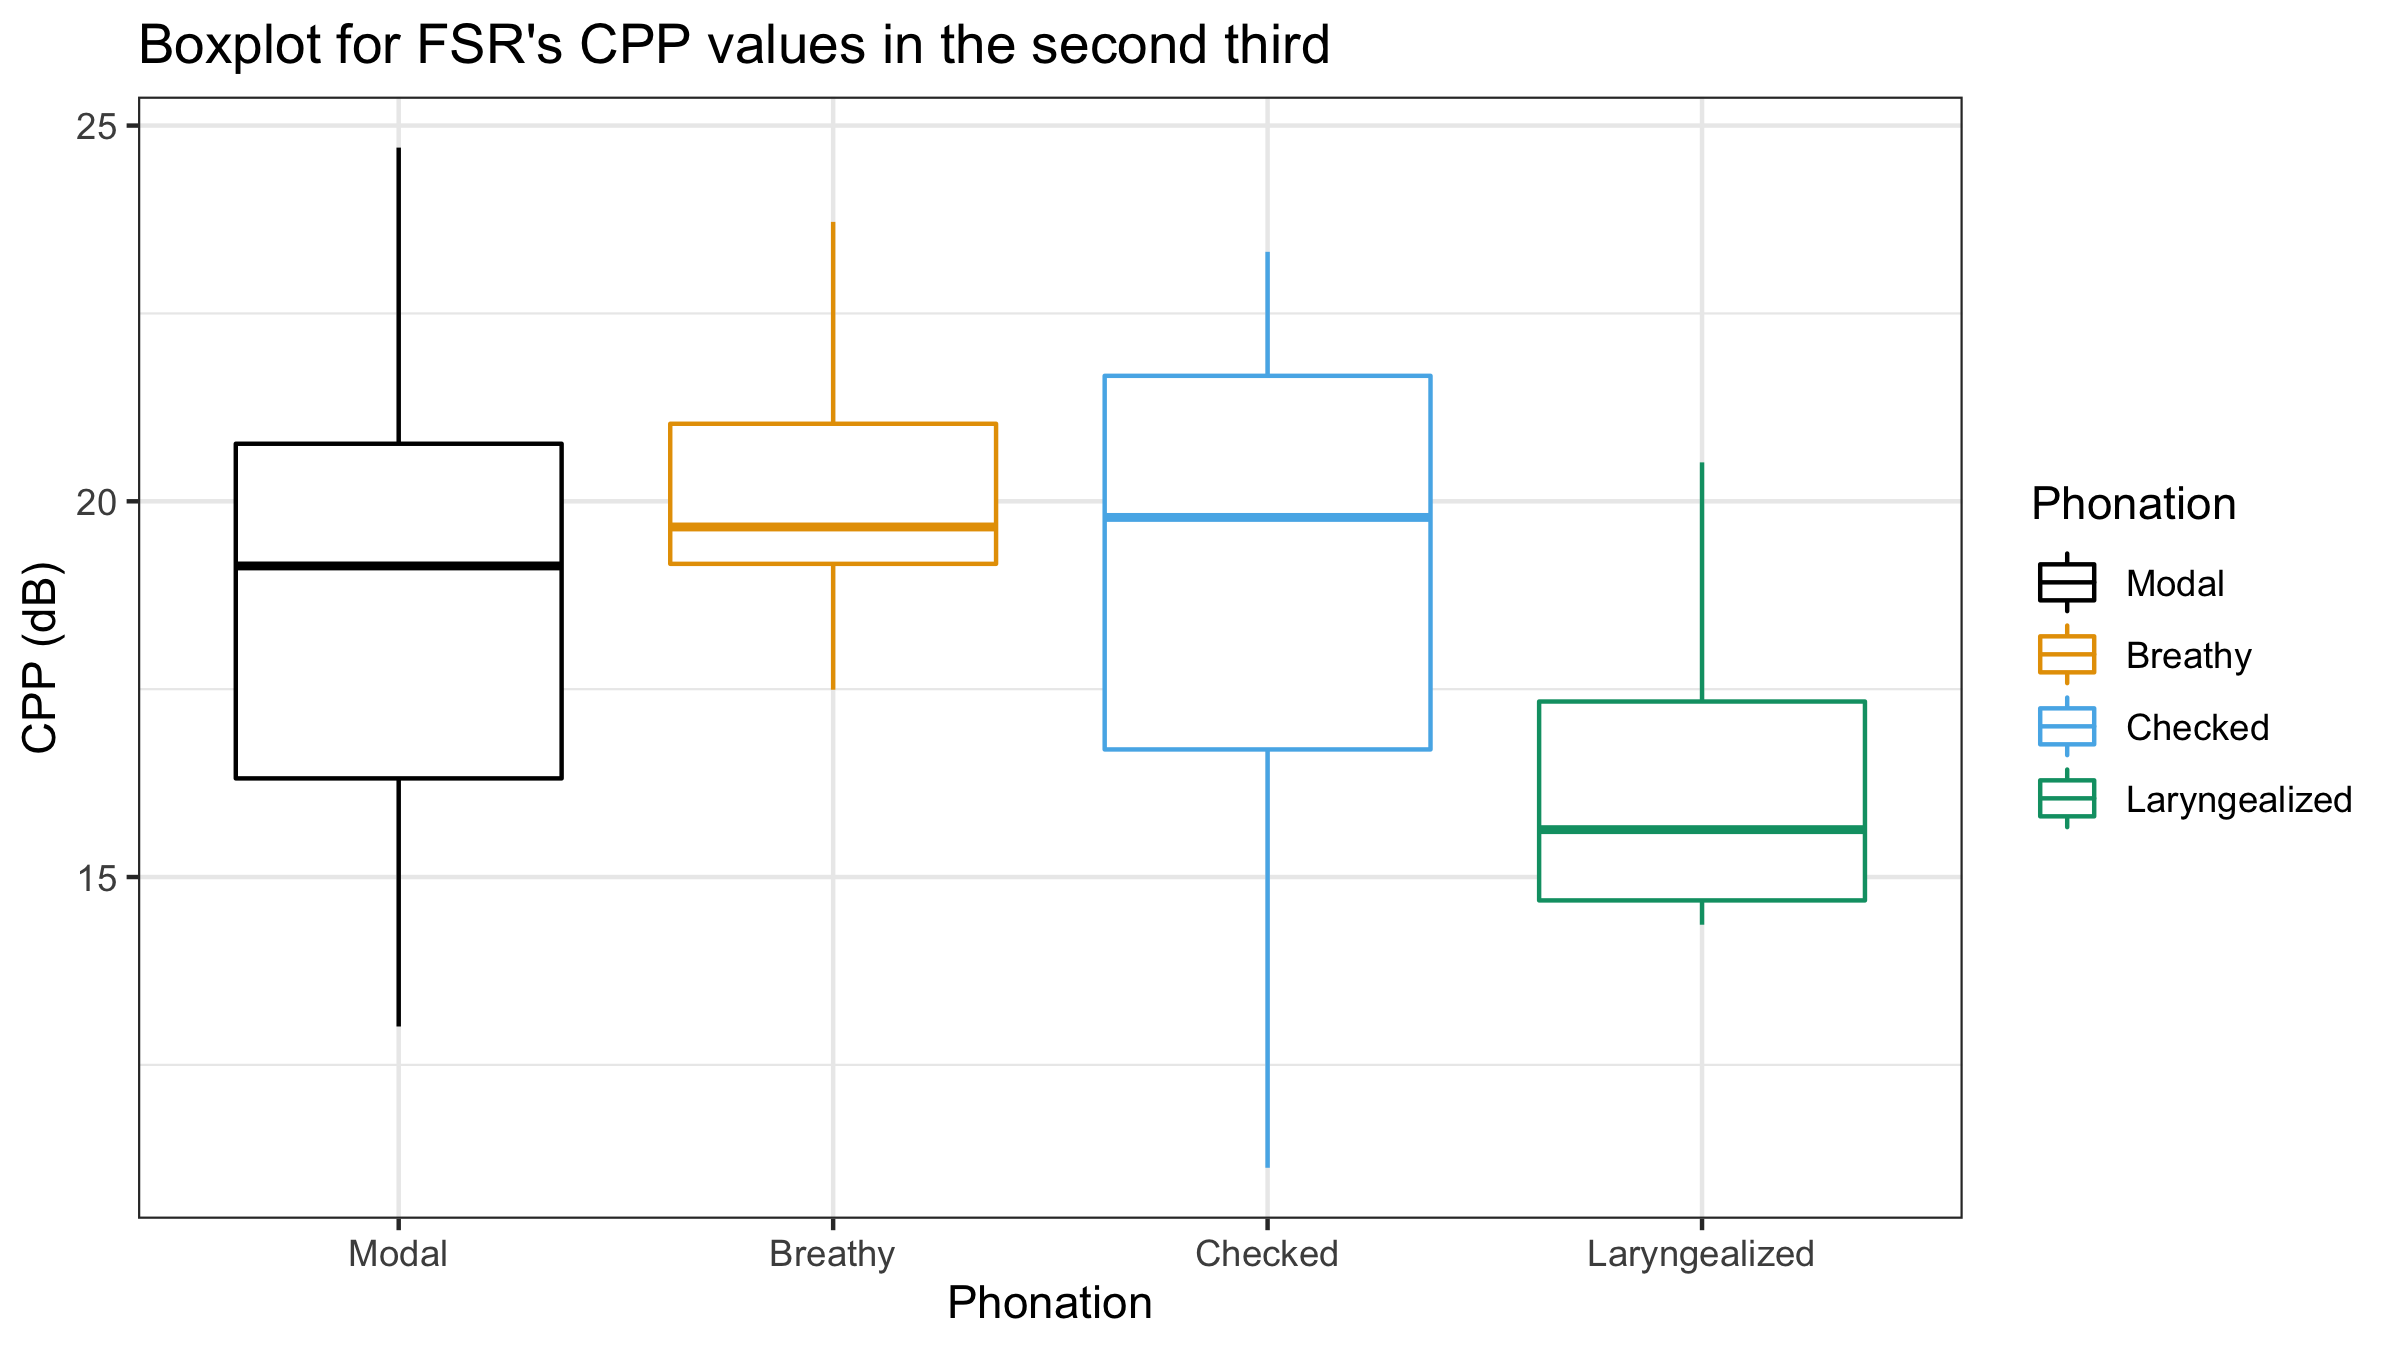
\includegraphics[width=0.9\textwidth]{Images/mean_FSR_cpp_Second.png}
		\caption{FSR's CPP values.}
		\label{fig:FSRcppsecond} 
	\end{subfigure}%
	\begin{subfigure}{.5\textwidth}
		\centering
		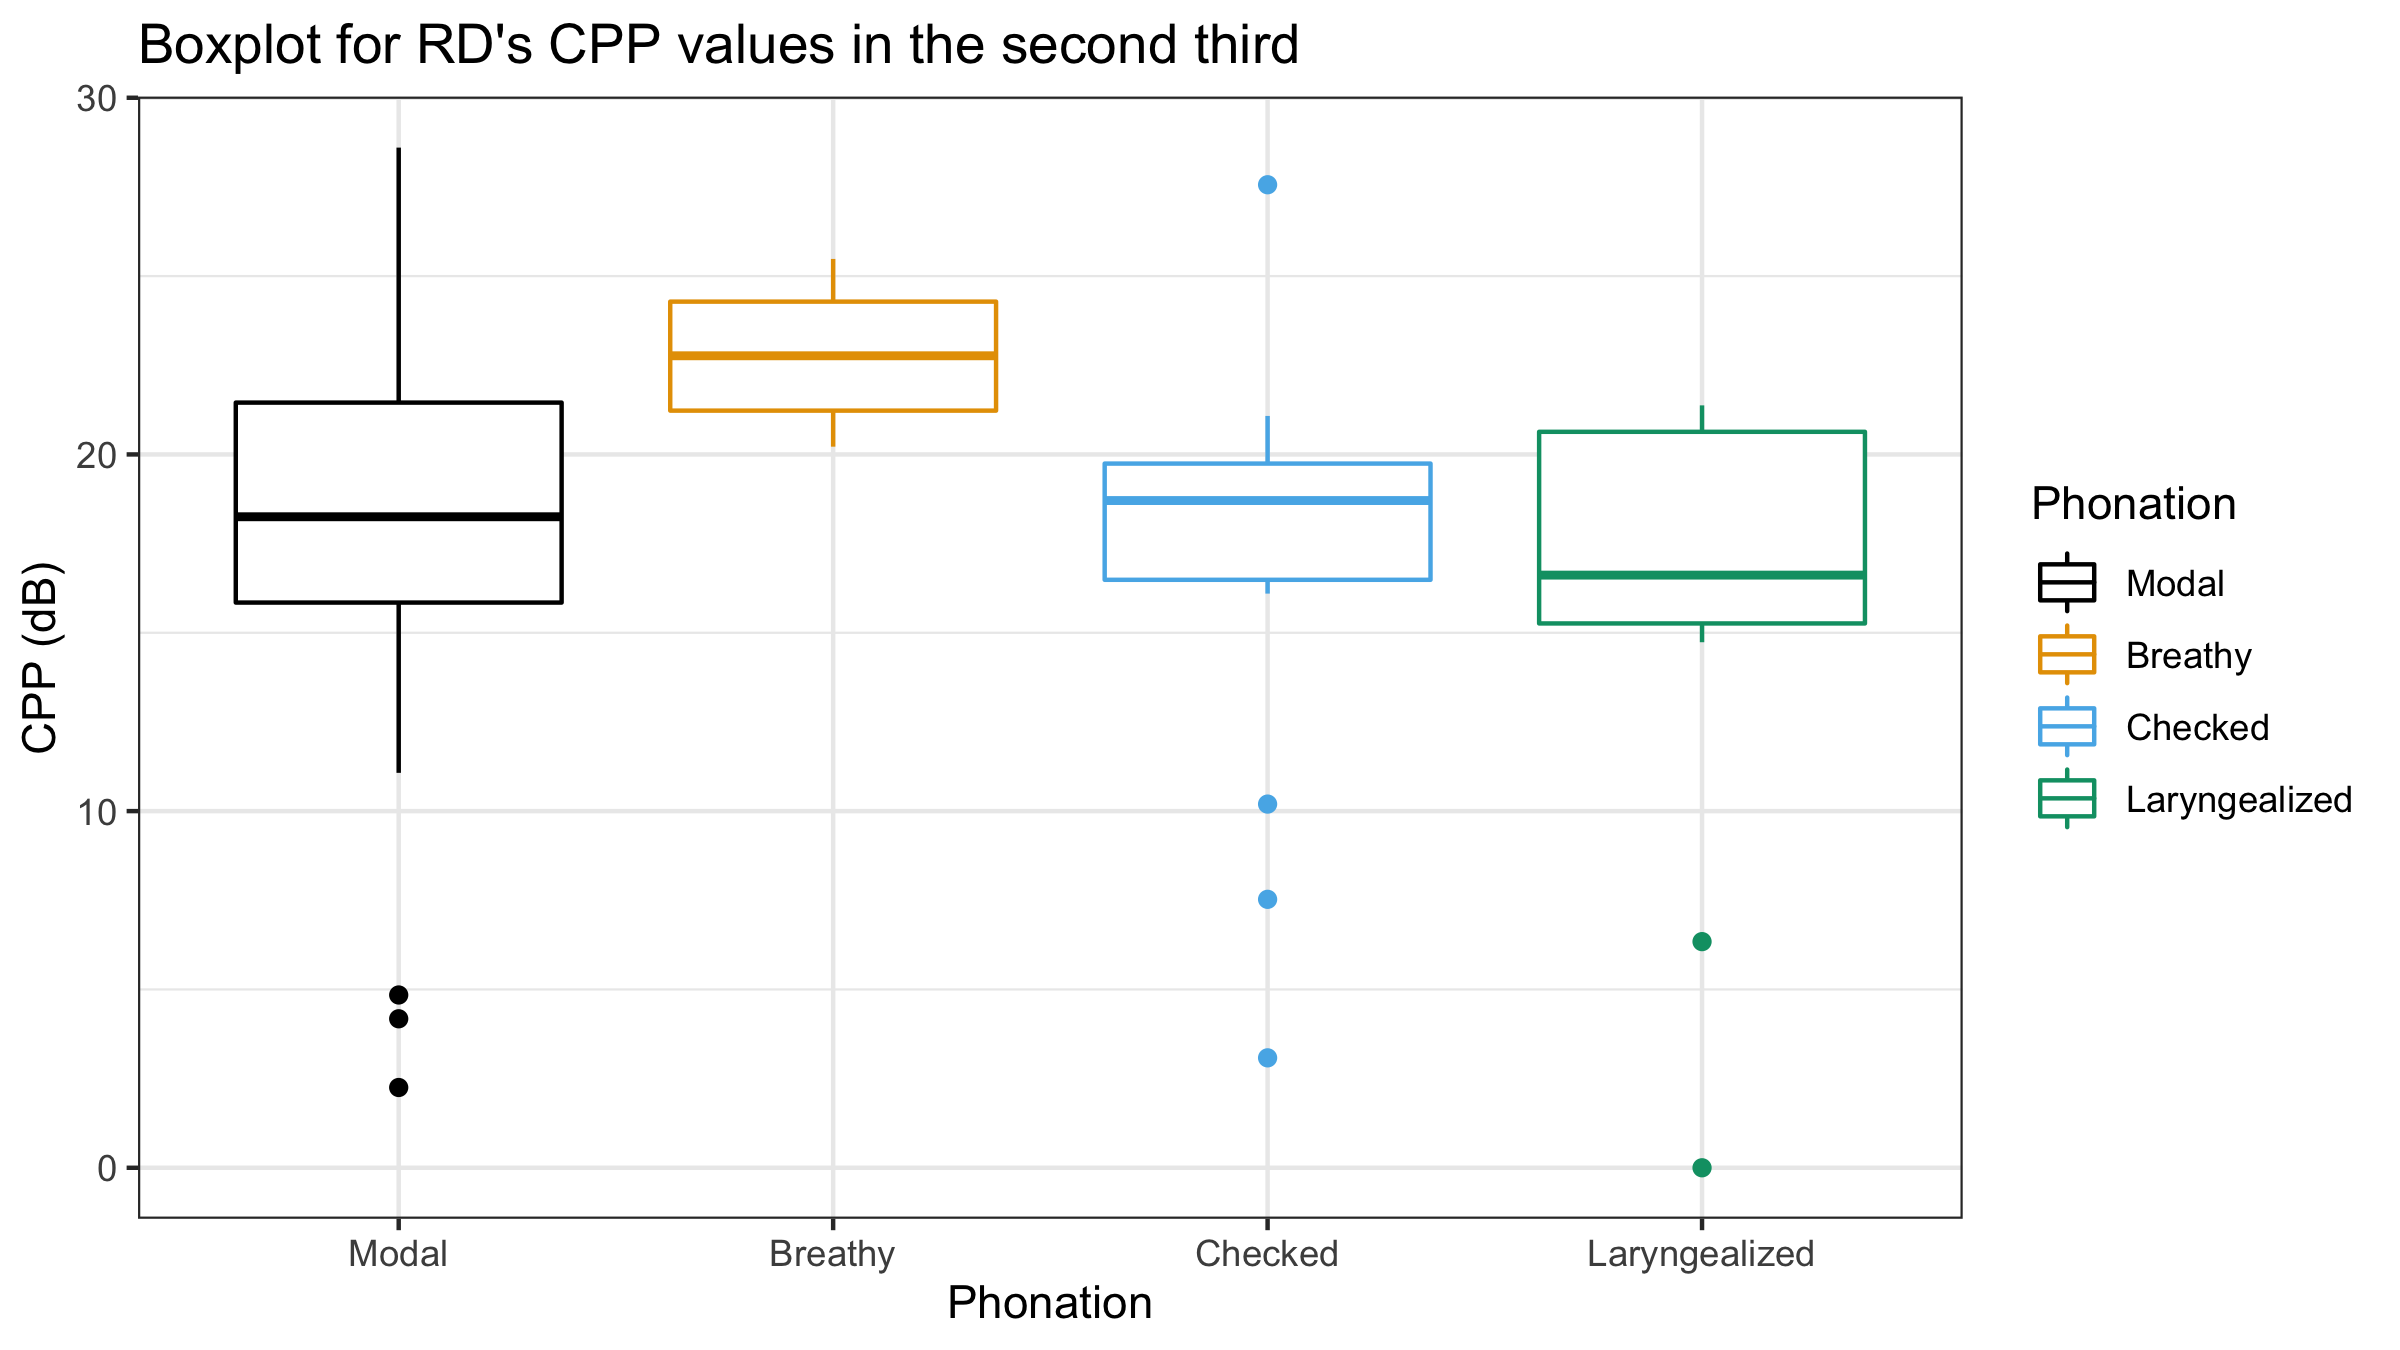
\includegraphics[width=0.9\textwidth]{Images/mean_RD_cpp_Second.png}
		\caption{RD's CPP values.}
		\label{fig:RDcppsecond} 
	\end{subfigure}
	\caption{CPP values for FSR (a) and RD (b) for the second third of the vowel. }
	\label{fig:cppsecond}
\end{figure}

\begin{figure}[!ht]
	\centering
	\begin{subfigure}{.5\textwidth}
		\centering
		\includegraphics[width=0.9\textwidth]{Images/mean_FSR_cpp_third.png}
		\caption{FSR's CPP values.}
		\label{fig:FSRcppthird} 
	\end{subfigure}%
	\begin{subfigure}{.5\textwidth}
		\centering
		\includegraphics[width=0.9\textwidth]{Images/mean_RD_cpp_third.png}
		\caption{RD's CPP values.}
		\label{fig:RDcppthird} 
	\end{subfigure}
	\caption{CPP values for FSR (a) and RD (b) for the final third of the vowel. }
	\label{fig:cppthird}
\end{figure}


%------------------------------------
\section{Statistical results} \label{sec:Stats}
%------------------------------------

In order to determine whether or not the different acoustic measurements were effective at capturing the different phonation types, a mixed-effects linear regression analysis was performed with Satterthwaite's method for t-test analysis used to derive the p-values. Each of the different measurements was treated as the dependent variable, with the word as the random variable. Because there were only two speakers, the statistical analysis was run for each speaker independently. In presenting the statistical analysis results, I present first the results of the mixed-effect linear regression for FSR then RD.

%------------------------------------
\subsection{FSR's Statistical results} \label{sec:FSRStats}
%------------------------------------

%------------------------------------
\subsubsection{H1-H2}
%------------------------------------

The first mixed-effects linear regression took the corrected H1-H2 values as the dependent variable, with each phonation type acting as a predictor. This analysis was then repeated for each third of the vowel. The statistical analysis results for FSR's H1-H2 values show that none of the values ever reach significance for the first third of the vowel; see Table~\ref{tab:FSR_H1H2_First}. 

\begin{table}[!h]
    \centering
    \caption{Results of the mixed-effects linear regression analysis on the first third of FSR's  vowel for H1-H2. }
    \label{tab:FSR_H1H2_First}
    \begin{tabular}{lllllll}
	\lsptoprule
					&  Estimate  & Std. Error & df & t value & p-value & \\
        Intercept       &  0.2591   & 0.3372 & 69.8456 & 0.768  & 0.445 & \\  
  	Breathy   		&  -0.9311  & 0.9829 & 75.9455 & -0.947  &  0.346 & \\
	Checked    		&  -0.5531  & 0.6344 & 60.0848 & -0.872  & 0.387 & \\
	Laryngealized	&  -0.7291  & 0.7547 & 70.7351 & -0.966  &  0.337 & \\
        \lspbottomrule
    \end{tabular}
\end{table}

When we turn to the results for the second portion of the vowel, we see that the lowered H1-H2 values that began in the middle of the vowel as seen in Section~\ref{sec:H1H2} were significant (Estimate = -5.1794, SE = 2.334, p = 0.0295). This means that when the H1-H2 value is lower than modal for FSR the vowel is breathy. 

\begin{table}[!h]
    \centering
    \caption{Results of the mixed-effects linear regression analysis on the second third of FSR's vowel for H1-H2. }
    \label{tab:FSR_H1H2_Second}
    \begin{tabular}{lllllll}
	\lsptoprule
					&  Estimate  & Std. Error & df & t value & p-value & \\
        Intercept       &  0.2054   & 0.8161 & 71.6610 & 0.252  & 0.8020  & \\  
  	Breathy   		&  -5.1794  & 2.3340 & 75.8687 & -2.219  &  0.0295 & *\\
	Checked    		&  -2.2631  & 1.4579 & 56.9101 & -1.552  & 0.1261  & \\
	Laryngealized	&  -0.2273  & 1.7642 & 69.9514 & -0.129  &  0.8978 & \\
        \lspbottomrule
    \end{tabular}
\end{table}

In the final third of the vowel, we observe that the lowered H1-H2 value for breathy vowels is significant again (Estimate = -3.5123, SE = 1.7417, p = 0.0473). However, unlike in the middle of the vowel, checked vowels also have a significantly lowered H1-H2 (Estimate = -2.2660, SE = 1.0636, p = 0.0382). This is to be expected because checked vowels have a glottal closure at the right edge of the vowel, which is sometimes realized as a small period of creakiness.

\begin{table}[!h]
    \centering
    \caption{Results of the mixed-effects linear regression analysis on the final third of FSR's vowel for H1-H2. }
    \label{tab:FSR_H1H2_Third}
    \begin{tabular}{lllllll}
	\lsptoprule
					&  Estimate  & Std. Error & df & t value & p-value & \\
        Intercept       &  -0.7772   & 0.6162 & 71.3050 & -1.261  & 0.2112  & \\  
  	Breathy   		&  -3.5123  & 1.7417 & 76.5774 & -2.017  &  0.0473 & *\\
	Checked    		&  -2.2660  & 1.0636 & 48.8779 & -2.130  & 0.0382 & * \\
	Laryngealized	&  -0.3561  & 1.2622 & 68.3544 & -0.282  &  0.7787 & \\
        \lspbottomrule
    \end{tabular}
\end{table}

What is surprising with these results is that both breathy and checked vowels are indicated with a lowered H1-H2. This is surprising because a lowered spectral-tilt measurement corresponds to a more closed glottis and, in turn, more creakiness in its articulation. What we should expect to see for breathy vowels is a higher spectral-tilt measurement

%------------------------------------
\subsubsection{H1-A3}
%------------------------------------

The measurement H1-A3 takes the amplitude of the first harmonic and subtracts the amplitude of the harmonic closest to the third formant. Similar to H1-H2, this spectral-tilt measurement can also be used to diagnose whether a vowel is breathy or creaky when compared to the value of H1-A3 for modal vowels. When we consider this measurement, we find that the breathy vowel has a significantly higher H1-A3 vowel throughout the whole vowel, the first third (Estimate = 5.3198, SE = 1.7202, p = 0.00277), second third (Estimate = 7.7803, SE = 3.1728, p = 0.016495), and final third (Estimate = 9.7176, SE = 2.5918, p = 0.000341). This higher spectral-tilt measurement corresponds to a more open glottis and a more breathy articulation of the vowel, which is what we expect to see for breathy vowels. 

\begin{table}[!h]
    \centering
    \caption{Results of the mixed-effects linear regression analysis on the first third of FSR's vowel for H1-A3. }
    \label{tab:FSR_H1A3_First}
    \begin{tabular}{lllllll}
	\lsptoprule
					&  Estimate  & Std. Error & df & t value & p-value & \\
        Intercept       &  1.6595  & 0.5843 & 76.0000 & 2.840  & 0.00578 & ** \\  
  	Breathy   		&  5.3198  & 1.7202 & 76.0000 & 3.093  & 0.00277 & **\\
	Checked    		&  0.8926  & 1.1248 & 76.0000 & 0.794  & 0.42993 & \\
	Laryngealized	&  0.1161  & 1.3301 & 76.0000 & 0.087  & 0.93068 & \\
        \lspbottomrule
    \end{tabular}
\end{table}

\begin{table}[!h]
    \centering
    \caption{Results of the mixed-effects linear regression analysis on the second third of FSR's vowel for H1-A3. }
    \label{tab:FSR_H1A3_Second}
    \begin{tabular}{lllllll}
	\lsptoprule
					&  Estimate  & Std. Error & df & t value & p-value & \\
        Intercept       &  3.8080  & 1.0778 & 76.0000 &  3.533  & 0.000702 & *** \\  
  	Breathy   		&  7.7803  & 3.1728 & 76.0000 &  2.452  & 0.016495 & *\\
	Checked    		&  0.8337  & 2.0748 & 76.0000 &  0.402  & 0.688934 & \\
	Laryngealized	& -0.7629  & 2.4534 & 76.0000 & -0.311  & 0.756697 & \\
        \lspbottomrule
    \end{tabular}
\end{table}

When we consider the other portions of the vowels and what they can tell us about the other phonation types, we see that only laryngealized vowels in the final third of the vowel ever reach significance. In the final third of the vowel, laryngealized vowels have a significantly higher H1-A3 than modal vowels by 4.2392dB (SE = 1.9356, p = 0.03154). This means that there is a more open constriction in the larynx during the final third of the vowel, corresponding to a more breathy phonation. Even though there is a higher H1-H2 it is in no ways has high as the value for truly breathy vowels. 

\begin{table}[!h]
    \centering
    \caption{Results of the mixed-effects linear regression analysis on the final third of FSR's vowel for H1-A3. }
    \label{tab:FSR_H1A3_Third}
    \begin{tabular}{lllllll}
	\lsptoprule
					&  Estimate  & Std. Error & df & t value & p-value & \\
        Intercept       &   5.0977  & 0.8804 & 77.0000 &  5.790  &  1.45e-7 & *** \\  
  	Breathy   		&   9.7176  & 2.5918 & 77.0000 &  3.749  &  0.000341 & ***\\
	Checked    		&  -1.2154  & 1.6948 & 77.0000 & -2.130  &  0.475465 &  \\
	Laryngealized	&   4.2392  & 1.9356 & 77.0000 & -0.282  &  0.031540 & * \\
        \lspbottomrule
    \end{tabular}
\end{table}

%------------------------------------
\subsubsection{CPP}
%------------------------------------

FSR's CPP values show an interesting effect. In the first third of the vowel, both laryngealized and breathy vowels have significantly elevated CPP values when compared to the modal vowel, with laryngealized vowels being 2.8175dB higher than 
modal vowels (SE = 1.2658, p = 0.02899). Breathy vowels are 4.9808db higher than modals (SE = 1.6370, p = 0.00322). If the reader can recall, the higher the CPP value, the more periodic the sound is. These higher CPP values mean that in the first third of the vowel, both breathy and laryngealized vowels are more periodic. 
\begin{table}[!h]
    \centering
    \caption{Results of the mixed-effects linear regression analysis on the first third of FSR's vowel for CPP. }
    \label{tab:FSR_CPP_First}
    \begin{tabular}{lllllll}
	\lsptoprule
					&  Estimate  & Std. Error & df & t value & p-value & \\
        Intercept       &  6.2773  & 0.5561 & 76.0000 & 11.289  & < 2e-16 & *** \\  
  	Breathy   		&  4.9808  & 1.6370 & 76.0000 & 3.093  & 0.00322  & **\\
	Checked    		& -0.7965  & 1.0705 & 76.0000 & 0.794  & 0.45913  & \\
	Laryngealized	&  2.8175  & 1.2658 & 76.0000 & 0.087  & 0.02899  & *\\
        \lspbottomrule
    \end{tabular}
\end{table}

When the vowel is in the second-third, the differences between the modal vowel and the breathy and checked phonation are insignificant. What is significant is that laryngealized vowels have a lower CPP score than modal vowels (Estimate = -2.365, SE = 0.9713, p = 0.0173). This lowered CPP value suggests that in the middle of FSR's vowels is a period of aperiodicity. 
\begin{table}[!h]
    \centering
    \caption{Results of the mixed-effects linear regression analysis on the second third of FSR's vowel for CPP. }
    \label{tab:FSR_CPP_Second}
    \begin{tabular}{lllllll}
	\lsptoprule
					&  Estimate  & Std. Error & df & t value & p-value & \\
        Intercept       & 18.7030  & 0.4324 & 74.5571 & 43.250  & < 2e-16  & *** \\  
  	Breathy   		&  1.5196  & 1.2630 & 75.9816 &  2.452  & 0.2327   & \\
	Checked    		& -0.2479  & 0.8176 & 69.7450 & -0.303  & 0.7626   & \\
	Laryngealized	& -2.3650  & 0.9713 & 74.0631 & -2.435  & 0.0173   & * \\
        \lspbottomrule
    \end{tabular}
\end{table}

In the final third of the vowel, only the lowered CPP value for checked vowels is significantly different from the modal vowel (Estimate = -1.7237, SE = 0.6767, p = 0.0154). This suggests that there is aperiodic noise at the end of checked vowels.

\begin{table}[!h]
    \centering
    \caption{Results of the mixed-effects linear regression analysis on the final third of FSR's vowel for CPP. }
    \label{tab:FSR_CPP_Third}
    \begin{tabular}{lllllll}
	\lsptoprule
					&  Estimate  & Std. Error & df & t value & p-value & \\
        Intercept       &  13.0737  & 0.3703 & 61.6759 & 35.303  & < 2e-16 & *** \\  
  	Breathy   		&   2.1004  & 1.0677 & 76.6308 &  1.967  &  0.0528 & .\\
	Checked    		&  -1.7237  & 0.6767 & 35.2715 & -2.547  &  0.0154 & * \\
	Laryngealized	&  -0.8860  & 0.7858 & 61.4343 & -1.128  &  0.2639 &  \\
        \lspbottomrule
    \end{tabular}
\end{table}

The results of FSR's CPP analysis show that both checked and laryngealized vowels produce aperiodic noise. Even though they are both characterized by this aperiodic noise, the difference seems to be in the timing of that aperiodic noise, with laryngealized vowels having it in the middle and checked vowels at the end of the vowel. 

%------------------------------------
\subsection{RD's Statistical results} \label{sec:RDStats}
%------------------------------------

%------------------------------------
\subsubsection{H1-H2}
%------------------------------------

The statistics from RD's H1-H2 show very little in terms of significance. In the first third of the vowel, checked vowels have a lower spectral-tilt than modal vowels (Estimate = -0.7284, SE = 0.3394, p = 0.0416). This lowered value disappears throughout the rest of the vowel. 

\begin{table}[!h]
    \centering
    \caption{Results of the mixed-effects linear regression analysis on the first third of RD's  vowel for H1-H2. }
    \label{tab:RD_H1H2_First}
    \begin{tabular}{lllllll}
	\lsptoprule
					&  Estimate  & Std. Error & df & t value & p-value & \\
        Intercept       &  1.4484 & 0.2373 & 58.9565 & 6.104 & 8.69e-08 & ***\\  
  	Breathy   		&  0.5909 & 0.5547 & 47.9027 & 1.065 & 0.2921 & \\
	Checked    		& -0.7284 & 0.3394 & 25.5118 & -2.146 & 0.0416 & * \\
	Laryngealized	&  0.3814 & 0.4481 & 53.4008 &  0.851 &  0.3985 & \\
        \lspbottomrule
    \end{tabular}
\end{table}

\begin{table}[!h]
    \centering
    \caption{Results of the mixed-effects linear regression analysis on the second third of RD's vowel for H1-H2. }
    \label{tab:RD_H1H2_Second}
    \begin{tabular}{lllllll}
	\lsptoprule
					&  Estimate  & Std. Error & df & t value & p-value & \\
        Intercept       &  3.7560  & 0.4421 & 62.4970 & 8.496 & 5.15e-12 & *** \\ 
  	Breathy   		&  -1.8288 & 1.2227 & 66.8127 & -1.496 & 0.139 &  \\
	Checked    		&  -1.3779 & 0.8663 & 59.3365 & -1.591 & 0.117  & \\
	Laryngealized	&  -1.5420 & 0.9514 & 65.9838 & -1.621 & 0.110 & \\
        \lspbottomrule
    \end{tabular}
\end{table}

In the final third of the vowel, we see that laryngealized vowels now have a significantly lower spectral-tilt measurement than modal vowels (Estimate = -1.726, SE = 0.7368, p = 0.0221).

\begin{table}[!h]
    \centering
    \caption{Results of the mixed-effects linear regression analysis on the final third of RD's vowel for H1-H2. }
    \label{tab:RD_H1H2_Third}
    \begin{tabular}{lllllll}
	\lsptoprule
					&  Estimate  & Std. Error & df & t value & p-value & \\
        Intercept       &  3.1024 & 0.3422 & 67.0000 & 9.066 & 2.91e-13 & *** \\  
  	Breathy   		& -1.3450 & 0.9475 & 67.0000 & -1.420 & 0.1604 &\\
	Checked    		& -0.7040 & 0.6721 & 67.0000 & -1.048 & 0.2986 & \\
	Laryngealized	& -1.7260 & 0.7368 & 67.0000 & -2.342 & 0.0221 & *\\
        \lspbottomrule
    \end{tabular}
\end{table}

%------------------------------------
\subsubsection{H1-A3}
%------------------------------------

When we consider the other spectral-tilt measurement of H1-A3, we see that breathy vowels have a significantly higher spectral-tilt measurement than modal vowels in the first third of the vowel (Estimate = 5.2731, SE = 1.7265, p = 0.00364) only even though the spectral-tilt measurement for breathy vowels is higher than modal vowels throughout the rest of the vowel it is only significantly different in that first third of the vowel. 

\begin{table}[!h]
    \centering
    \caption{Results of the mixed-effects linear regression analysis on the first third of RD's  vowel for H1-A3. }
    \label{tab:RD_H1A3_First}
    \begin{tabular}{lllllll}
	\lsptoprule
					&  Estimate  & Std. Error & df & t value & p-value & \\
        Intercept       &  5.9391 & 0.7388 & 59.5527 & 8.039 & 4.42e-11 & *** \\  
  	Breathy   		&  5.2731 & 1.7265 & 49.0198 & 3.054 & 0.00364 & **\\
	Checked    		& -1.0449 & 1.0562 & 26.8824 & -0.989 & 0.33134 & \\
	Laryngealized	& -0.5252 & 1.3948 & 54.2691 & -0.377 & 0.70798 & \\
        \lspbottomrule
    \end{tabular}
\end{table}

\begin{table}[!h]
    \centering
    \caption{Results of the mixed-effects linear regression analysis on the second third of RD's vowel for H1-A3. }
    \label{tab:RD_H1A3_Second}
    \begin{tabular}{lllllll}
	\lsptoprule
					&  Estimate  & Std. Error & df & t value & p-value & \\
        Intercept       & 18.0631 & 0.9229 & 67.0000 & 19.571 & <2e-16 & *** \\  
  	Breathy   		&  3.9222 & 2.5555 & 67.0000 &  1.535 & 0.130 & \\
	Checked    		&  1.6654 & 1.8126 & 67.0000 & 0.919 & 0.361 & \\
	Laryngealized	& -4.6979 & 1.9873 & 67.0000 & -2.364 & 0.021 & * \\
        \lspbottomrule
    \end{tabular}
\end{table}

In the final third of the vowel, we see that laryngealized vowels are marked with a significantly lower spectral-tilt measurement than modal vowels (Estimate = -4.0282, SE = 1.7891, p = 0.0276). 

\begin{table}[!h]
    \centering
    \caption{Results of the mixed-effects linear regression analysis on the final third of RD's vowel for H1-A3. }
    \label{tab:RD_H1A3_Third}
    \begin{tabular}{lllllll}
	\lsptoprule
					&  Estimate  & Std. Error & df & t value & p-value & \\
        Intercept       & 14.6608 & 0.8309 & 67.0000 & 17.645 & <2e-16 & *** \\
  	Breathy   		&  3.1744 & 2.3006 & 67.0000 &  1.380 &  0.1722 & \\
	Checked    		& -0.2186 & 1.6318 & 67.0000 & -0.134 &  0.8938 &  \\
	Laryngealized	& -4.0282 & 1.7891 & 67.0000 & -2.252 &  0.0276 & * \\
        \lspbottomrule
    \end{tabular}
\end{table}

%------------------------------------
\subsubsection{CPP}
%------------------------------------

RD's CPP values, however, were not very informative for the different phonation types. Similar to FSR's CPP values in the first third of the vowel, breathy vowels have significantly higher CPP values than modal vowels (Estimate = 3.2595, SE = 1.6092, p = 0.0483). In contrast to FSR, this elevated CPP value for breathy vowels continues throughout the second third of the vowel (Estimate = 4.9411, SE = 2.4428, p = 0.0471). This suggests that the breathy vowels are more periodic than modal vowels. As for the other amodal phonation types, even though they have lower CPP values than modal vowels throughout all portions of the vowels, this difference never reaches significance. 

\begin{table}[!h]
    \centering
    \caption{Results of the mixed-effects linear regression analysis on the first third of RD's  vowel for CPP. }
    \label{tab:RD_CPP_First}
    \begin{tabular}{lllllll}
	\lsptoprule
					&  Estimate  & Std. Error & df & t value & p-value & \\
        Intercept       &  5.2213 & 0.6826 & 58.9564 & 7.649 & 2.16e-10 & *** \\  
  	Breathy   		&  3.2595 & 1.6092 & 48.8223 & 2.026 & 0.0483 & *\\
	Checked    		& -1.8668 & 0.9901 & 25.8528 & -1.886 & 0.0706 & . \\
	Laryngealized	&  -0.5991 & 1.2986 & 54.3588 & -0.461 & 0.6464 &\\
        \lspbottomrule
    \end{tabular}
\end{table}

\begin{table}[!h]
    \centering
    \caption{Results of the mixed-effects linear regression analysis on the second third of RD's vowel for CPP. }
    \label{tab:RD_CPP_Second}
    \begin{tabular}{lllllll}
	\lsptoprule
					&  Estimate  & Std. Error & df & t value & p-value & \\
        Intercept       & 17.8312 & 0.8877 & 63.0360 & 20.086 & <2e-16 & *** \\  
  	Breathy   		&  4.9411 & 2.4428 & 66.7464 & 2.023 & 0.0471 & * \\
	Checked    		&  -0.8325 & 1.7223 & 59.0340 & -0.483 & 0.6306 & \\
	Laryngealized	& -2.0799 & 1.9058 & 66.4538 & -1.091 &  0.2791 & \\
        \lspbottomrule
    \end{tabular}
\end{table}

\begin{table}[!h]
    \centering
    \caption{Results of the mixed-effects linear regression analysis on the final third of RD's vowel for CPP. }
    \label{tab:RD_CPP_Third}
    \begin{tabular}{lllllll}
	\lsptoprule
					&  Estimate  & Std. Error & df & t value & p-value & \\
        Intercept       & 10.7243 & 0.6256 & 61.5739 & 17.141 & <2e-16 & *** \\  
  	Breathy   		& 2.8325  & 1.6232 & 63.1367 &  1.745 &  0.0859 & .\\
	Checked    		& -2.1291 & 1.0790 & 42.1613 & -1.973 &  0.0551 & . \\
	Laryngealized	& -1.2433 & 1.2896 & 65.8635 & -0.964 &  0.3385 &  \\
        \lspbottomrule
    \end{tabular}
\end{table}

%------------------------------------
\section{Discussion} \label{sec:Discussion}
%------------------------------------

Based on the results of the spectral-tilt measurements, there is some agreement and disagreement with established patterns in what measures capture the different phonations best. 

Contrary to \citet{espositoVariationContrastivePhonation2010}, H1-H2 was not the best measurement for all phonation contrasts for the female SLZ speaker. FSR's breathy vowels were best measured using H1-A3. This fact suggests several things. We can first surmise that H1-H2 is not always the best measurement for phonation. This aligns with more recent findings that H1-H2 is a poor measure of phonation in general \citep{chaiH1H2Acoustic2022}. H2 is sensitive to differences in subglottal pressure \citep{sundbergObjectiveCharacterizationPhonation2022}. We can surmise this because breathy phonation had a very low value, which is opposite from what is commonly expected, a higher value than the modal's value. Additionally, the only time this measure behaved in a way that we expected was for FSR's checked vowels. In the final third of the vowel, the lower H1-H2 measure indicates a period of creakiness that corresponds with the glottal closure accompanying these vowels. 

This behavior of H1-H2 also suggests that \posscitet{espositoVariationContrastivePhonation2010} observation that H1-H2 is best for female speakers of Santa Ana del Valle Zapotec and H1-A3 for males might not apply to all varieties of Zapotec. However, there remains a large amount of work to confirm the results of this study. Primarily, this work was based on the results of only two speakers. More speakers can be consulted now that the COVID-19 pandemic has decreased in severity, and most of Santiago Laxopa has been vaccinated. This is especially important because it will allow researchers to understand better how laryngealized vowels are produced and what cues help differentiate them. 

This fact concerning laryngealized vowels is especially true given that FSR's spectral-tilt measurements for laryngealized vowels were nearly identical to those for modal vowels. However, one important thing is that we still got a lower CPP vowel in the second-third of the vowel in these laryngealized vowels. This position is precisely where one would expect acoustic cues for aperiodic noise. Additionally, we see in the spectrograms for these laryngealized vowels a decrease in amplitude for some time. This decrease in amplitude is significant because \citet{gerfenProductionPerceptionLaryngealized2005} found that even a slight reduction in amplitude was enough for people to identify a glottal stop. When we consider RD's measurements for laryngealized vowels, which RD consistently produces with creaky voice, we find that this vowel shows a consistently lower H1-A3 beginning in the middle of the vowel and continuing throughout the rest of the vowel. This pattern matches what one would expect to see.

These findings answer some questions but raise several others. The questions it answers concern the most reliable cues to phonation. It shows that languages are not uniform in relying on the same spectral-tilt measurements and types of harmonics-to-noise but that each language may make use of different types and combinations of these measurements to cue phonation, which seems to be somewhat more analogous to the varying ways in which languages realize voicing contrasts \citep{liskerCrossLanguageStudyVoicing1964}. It is well known that English's voicing contrast is a difference in voiceless plain stops and voiceless aspirated stops in word-initial position. In contrast, languages like Dutch and Spanish make an actual voicing distinction. 

Another question has to do with the predictions from the Laryngeal Complexity Hypothesis. The \textsc{Laryngeal Complexity Hypothesis} (LCH) has its origins in work by \citet{silvermanLaryngealComplexityOtomanguean1997,blankenshipTimeCourseBreathiness1997,blankenshipTimingNonmodalPhonation2002}. The basic premise of the LCH is that in languages that have both tone and phonation, there needs to be an ordering between the two laryngeal gestures for tone and phonation for optimal perceptibility. This premise comes from the understanding that the same mechanism responsible for tone is also responsible for the production of phonation: the vocal folds and glottis. The rate at which vocal folds vibrate is responsible for changing the fundamental frequency, perceived as pitch, which is grammaticalized as tone in lexical tone languages. The faster the vocal folds vibrate, the higher the pitch. And the slower the vocal folds vibrate, the lower the pitch. 

The vocal folds are also the primary articulator for phonation. \citet{ladefogedPreliminariesLinguisticPhonetics1971,gordonPhonationTypesCrosslinguistic2001} treated phonation as a by-product of how open or closed the glottis is during vocal fold vibration. This is schematized by Figure~\ref{fig:Phonation}. The more open the glottis is, the breathier the sound to the point where the sound becomes the sound [h]. The more closed the glottis is, the creakier the sound is to the point where the sound becomes [ʔ]. 

\begin{figure}[!ht]
	\centering
	\includegraphics[width=.6\textwidth]{Phonation.png}
	\caption{Simplified one-dimensional model for phonation. Based on \citet{ladefogedPreliminariesLinguisticPhonetics1971,gordonPhonationTypesCrosslinguistic2001}}.
	\label{fig:Phonation2}
\end{figure}

The LCH assumes phonation and tone are produced at the vocal folds and glottis. Because these same organs are responsible for these two phenomena, a mismatch exists in trying to have both simultaneously. It is assumed by the LCH that because of this issue, there needs to be strict ordering in the glottal gestures. This means the tonal gesture must be produced before or after the phonation gesture. The reason for this is that if the gestures overlap, there will be a perturbation of the tone, and the listeners will not be able to differentiate the tone reliably. The LCH assumes that there is a close link between production and perception. This assumption places the responsibility on making sure the acoustic cues are the most perceptually salient on the speaker. The speaker is responsible for producing both tone and phonation so that the listener can differentiate the different cues for both tone and phonation. These assumptions can best be represented by Figure~\ref{fig:GlottalGestures}. 

In Figure~\ref{fig:GlottalGestures}, which is taken from \citet{dicanioCoarticulationToneGlottal2012}, the cue for tone is represented by the Pitch Target and the Glottal Gesture represents the gestures needed to produce phonation. When the Pitch Target is not co-articulated with the Glottal Gestures, there is the greatest perceptual recoverability for the listener. The LCH argues for this as the tones are the most recoverable on modal vowels. This modal portion is then ordered or phased relative to the non-modal portion. This ordering is the speaker's responsibility to accommodate the listeners' perceptibility. If, however, the Pitch Target and the Glottal Gesture were overlapping, as represented by the lower half in Figure~\ref{fig:GlottalGestures}, then the cues for pitch and phonation would be overlapping and making it perceptually more difficult for 
\begin{figure}[!ht]
	\centering
	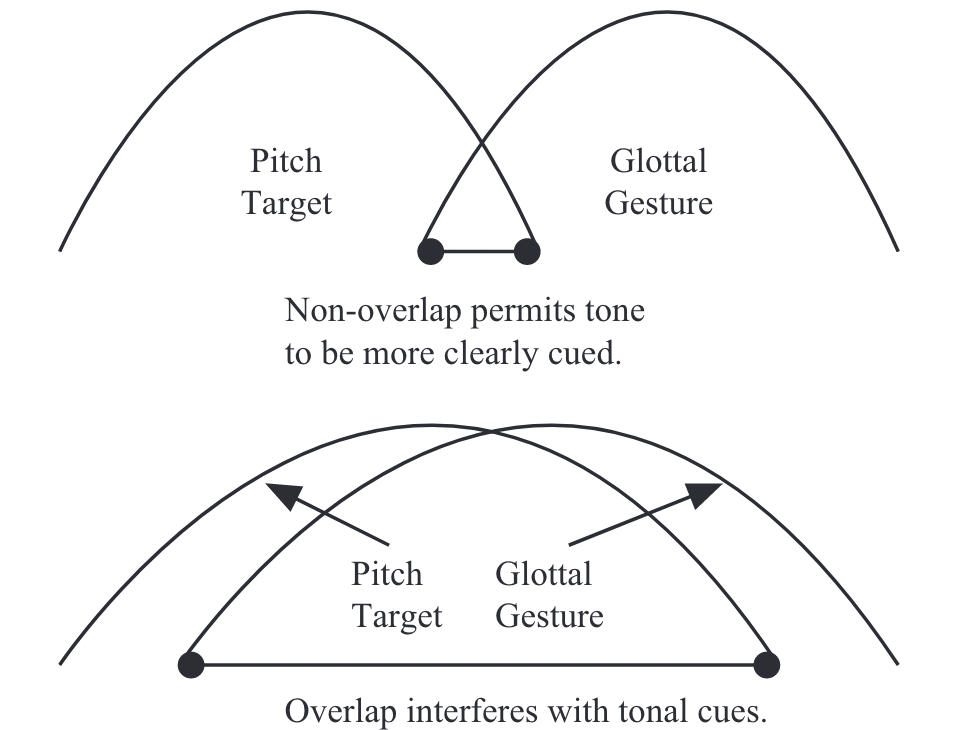
\includegraphics[width=.5\textwidth]{Gestures.png}
	\caption{Representation taken from \citet{dicanioCoarticulationToneGlottal2012}.}
	\label{fig:GlottalGestures}
\end{figure}

Some work has been done investigating this in other languages, most notably \posscitet{dicanioCoarticulationToneGlottal2012} investigation into glottals in Itunyoso Trique, which is also an Oto-Manguean language. \citeauthor{dicanioCoarticulationToneGlottal2012} in his study found that when the magnitude of coarticulation for glottal consonants occurs on the vowels, there is a strong correlation between the magnitude of overlap and the amount of perturbation in the f0 signal. If the degree of overlap was minor, then the acoustic signal had little to no perturbation. These results were found by consulting the spectral tilt of the vowels with the f0 measures and performing a generalized linear mixed effects model with the speaker treated as a random effect. 

Another study on Jalapa Mazatec \citep{garellekAcousticConsequencesPhonation2011} also investigated the interaction of tone and phonation. Jalapa Mazatec is a language with both contrastive tone and phonation, and \citet{garellekAcousticConsequencesPhonation2011} validated the claims made by the LCH, in that tone and phonation seemed to be ordered with each other when it comes to at least one of the phonation types. 

This paper describes the tonal and phonation inventories in Santiago Laxopa Zapotec, an ideal language for testing the viability of the LCH because of its use of both contrastive tone and contrastive phonation.   

Another question this study raises is the status of laryngealized vowels and their realizations. We observed from just two speakers that these vowels are highly variable. Assuming that \posscitet{avelinoAcousticElectroglottographicAnalyses2010} observations on this vowel in the closely related Yalálag Zapotec hold in SLZ, there is considerably more variation that exists within and between speakers. Suppose all of these varying realizations of a phonological category are evident. What does this mean for this category's status and the cues necessary for speakers to produce and realize this category? 

%------------------------------------
\section{Conclusion} \label{sec:Conclusion}
%------------------------------------

In conclusion, this paper has briefly introduced the tonal and phonation systems of Santiago Laxopa Zapotec, an understudied variety of Sierra Norte Zapotec. This system is essential for exploring the acoustic cues used in different languages to differentiate each phonation type.

Contrary to acoustic work on other Zapotec varieties by \citet{espositoVariationContrastivePhonation2010}, which showed that female speakers' phonation contrasts were best characterized by H1-H2 and male speakers' contrasts by H1-A3, SLZ suggests that both male and female speakers' breathy voice is best described by H1-A3 and checked and laryngealized voice are characterized by a difference in the timing of spectral-tilt measurements and CPP values depending on the speaker. 

Because of these phonation type differences in behavior, one could, in theory, speak to how SLZ compensates for using the larynx for both tone and phonation. This paper has not explicitly spoken on this issue, and the Laryngeal Complexity Hypothesis presented by \citet{silvermanLaryngealComplexityOtomanguean1997} and \citet{blankenshipTimeCourseBreathiness1997, blankenshipTimingNonmodalPhonation2002}. The LCH states that when a language has tone and phonation, these different aspects are ordered or phased concerning one another. This phasing allows for the most significant perceptibility in the acoustic signal. This allows the listener to adequately interpret the acoustic signals for tone and phonation. 

Overall, there seems to be some information from the spectral-tilt and CPP analysis that speaks to the question of the LCH. If the reader recalls, CPP was the most important cue for differentiating checked and laryngealized vowels from modal and breathy vowels for FSR. The key is the lower CPP value, which corresponds to greater aperiodicity. It is worth repeating that we did see a difference in the timing of the aperiodicity between checked and laryngealized vowels. In laryngealized vowels, this dip in CPP occurs in the middle third of the vowel, and for checked vowels, this dip occurs in the final third. However, the fact that for breathy vowels, the most noticeable cue is the higher H1-A3 which happens throughout the entire vowel, might suggest that breathiness does not behave in the same way as the other phonation types. The behavior from checked and laryngealized vowels seems to support the LCH. Unfortunately, no firm conclusions can be made about the LCH, and further investigation is required to determine the validity of the LCH in SLZ. 

This ability of speakers to interpret the acoustic signals in conjunction with the acoustic signals for tone is of great interest. It would benefit from a perception experiment to determine what the speakers are using to differentiate the different phonation types. This is especially true for laryngealized vowels, which have such varied pronunciations. 

This study will benefit from further analysis and data collection. Now that the world is safer regarding COVID-19, collecting data from more speakers is essential to corroborate the data and analysis from FSR and RD. 

%------------------------------------
%BIBLIOGRAPHY
%------------------------------------

%\singlespacing
% \nocite{*}
\printbibliography[heading=bibintoc]

\end{document}